%%%%%%%%%%%%%%%%%%%%%%%%%%%%%%%%%%%%%%%%%
% Beamer Presentation
% LaTeX Template
% Version 1.0 (10/11/12)
%
% This template has been downloaded from:
% http://www.LaTeXTemplates.com
%
% License:
% CC BY-NC-SA 3.0 (http://creativecommons.org/licenses/by-nc-sa/3.0/)
%
%%%%%%%%%%%%%%%%%%%%%%%%%%%%%%%%%%%%%%%%%

%----------------------------------------------------------------------------------------
%	PACKAGES AND THEMES
%----------------------------------------------------------------------------------------

\documentclass{beamer}

\mode<presentation> {

% The Beamer class comes with a number of default slide themes
% which change the colors and layouts of slides. Below this is a list
% of all the themes, uncomment each in turn to see what they look like.

%\usetheme{default}
%\usetheme{AnnArbor}
%\usetheme{Antibes}
% \usetheme{Bergen}
%\usetheme{Berkeley}
%\usetheme{Berlin}
%\usetheme{Boadilla}
% \usetheme{CambridgeUS}
%\usetheme{Copenhagen}
%\usetheme{Darmstadt}
%\usetheme{Dresden}
%\usetheme{Frankfurt}
%\usetheme{Goettingen}
%\usetheme{Hannover}
%\usetheme{Ilmenau}
%\usetheme{JuanLesPins}
%\usetheme{Luebeck}
% \usetheme{Madrid}
%\usetheme{Malmoe}
%\usetheme{Marburg}
%\usetheme{Montpellier}
%\usetheme{PaloAlto}
%\usetheme{Pittsburgh}
%\usetheme{Rochester}
%\usetheme{Singapore}
\usetheme{Szeged}
%\usetheme{Warsaw}

% As well as themes, the Beamer class has a number of color themes
% for any slide theme. Uncomment each of these in turn to see how it
% changes the colors of your current slide theme.

% \usecolortheme{albatross}
% \usecolortheme{beaver}
% \usecolortheme{beetle}
% \usecolortheme{crane}
\usecolortheme{dolphin}
% \usecolortheme{dove}
% \usecolortheme{fly}
% \usecolortheme{lily}
% \usecolortheme{orchid}
% \usecolortheme{rose}
% \usecolortheme{seagull}
%\usecolortheme{seahorse}
% \usecolortheme{whale}
%\usecolortheme{wolverine}

%\setbeamertemplate{footline} % To remove the footer line in all slides uncomment this line
\setbeamertemplate{footline}[page number] % To replace the footer line in all slides with a simple slide count uncomment this line

\setbeamertemplate{navigation symbols}{} % To remove the navigation symbols from the bottom of all slides uncomment this line
}

\setbeamercolor{framesource}{fg=gray}
\setbeamerfont{framesource}{size=\tiny}
\usefonttheme[onlymath]{serif}

\usepackage{graphicx} % Allows including images
\usepackage{booktabs} % Allows the use of \toprule, \midrule and \bottomrule in tables
\usepackage[absolute,overlay]{textpos}
\usepackage{appendixnumberbeamer}
\usepackage{amsmath}

\usepackage{pgfpages}
\setbeameroption{show notes on second screen}

%----------------------------------------------------------------------------------------
% Commands used in this presentation
%----------------------------------------------------------------------------------------

% Lower right image citation
\newcommand{\source}[1]{\begin{textblock*}{4cm}(8.7cm,8.6cm)
    \begin{beamercolorbox}[ht=0.5cm,right]{framesource}
        \usebeamerfont{framesource}\usebeamercolor[fg]{framesource} Source: {#1}
    \end{beamercolorbox}
\end{textblock*}}

\newcommand{\sourceleft}[1]{\begin{textblock*}{4cm}(.4cm,8.6cm)
    \begin{beamercolorbox}[ht=0.5cm,left]{framesource}
        \usebeamerfont{framesource}\usebeamercolor[fg]{framesource} Source: {#1}
    \end{beamercolorbox}
\end{textblock*}}

% Images in place of math
\newcommand{\mysymbol}[1]{\mathord{\includegraphics[height=1.6cm]{image/#1}}}


%----------------------------------------------------------------------------------------
%	TITLE PAGE
%----------------------------------------------------------------------------------------

\title[Predoctoral Defense]{Bayesian inference methodologies to reconstruct the evolution and spread of pathogens} % The short title appears at the bottom of every slide, the full title is only on the title page

\author{Barney I. Potter} % Your name
\institute[KU Leuven] % Your institution as it will appear on the bottom of every slide, may be shorthand to save space
{
KU Leuven \\ % Your institution for the title page
\medskip
Supervisors: Prof.~Dr.~G. Baele, Dr.~M. Gill\\
Jury: Prof.~Dr.~G. Opdenakker, Prof.~Dr.~P. Lemey, Prof.~Dr.~J. Matthijnssens, Prof.~Dr.~L. Dupont
}
\titlegraphic{
\includegraphics[height=1.8cm]{image/KULEUVEN_LOGO_2012}}
\date{\today} % Date, can be changed to a custom date

% \logo{
\includegraphics[height=.3cm]{image/KULEUVEN_LOGO_2012.pdf}\vspace{225pt}}

\begin{document}

\begin{frame}
  \titlepage % Print the title page as the first slide
  \note[item]{Thank everyone for being here}
\end{frame}

% \begin{frame}
% \frametitle{Overview} % Table of contents slide, comment this block out to remove it
% \colorbox{red}{REMOVE THIS SLIDE FOR FINAL VERSION}
% \tableofcontents % Throughout your presentation, if you choose to use \section{} and \subsection{} commands, these will automatically be printed on this slide as an overview of your presentation
% \end{frame}

%----------------------------------------------------------------------------------------
%	PRESENTATION SLIDES
%----------------------------------------------------------------------------------------

%------------------------------------------------
\section{Introduction} % Sections can be created in order to organize your presentation into discrete blocks, all sections and subsections are automatically printed in the table of contents as an overview of the talk
%------------------------------------------------

\begin{frame}

  \frametitle{Emerging infectious diseases}
  \begin{figure}
    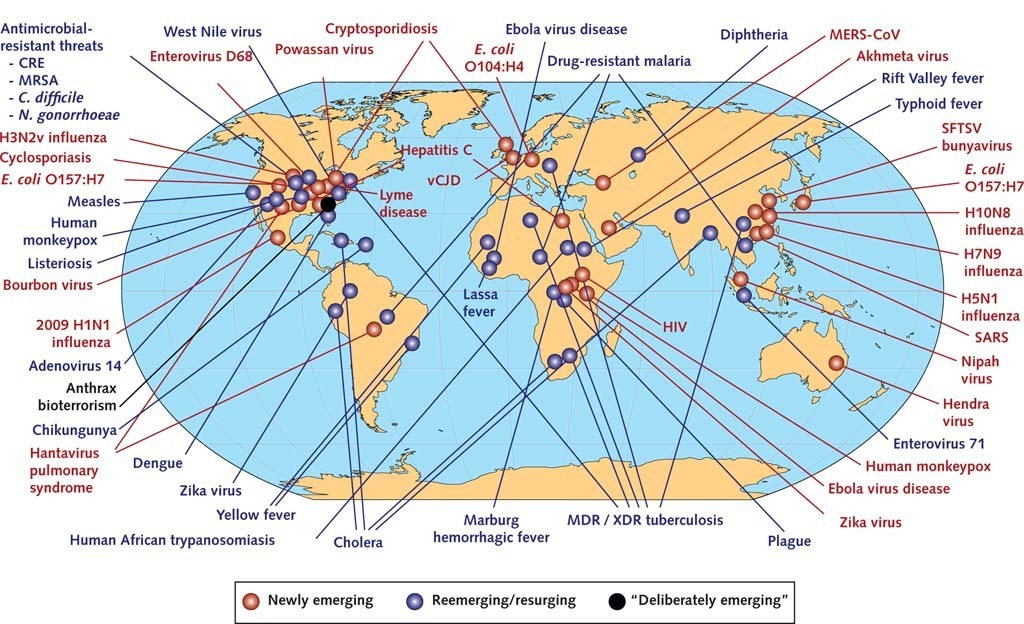
\includegraphics[width=.95\linewidth]{image/intro/eids}
    \source{Paules et al. (2017)}
  \end{figure}

  \note[item]{Increasingly interconnected, population dense world leads to more EIDs}
  \note[item]{Range from isolated outbreaks (MRSA, MERS) to epidemics of regional scales (West African Ebola, Zika in the America) to pandemics (SARS-CoV-2)}
  \note[item]{As EIDs continue to increasingly affect global public health, we need to develop new tools to characterize them and inform public health interventions}

\end{frame}

%------------------------------------------------

\begin{frame}

  \frametitle{Virus evolution mirrors the epidemic process}
  \begin{figure}
    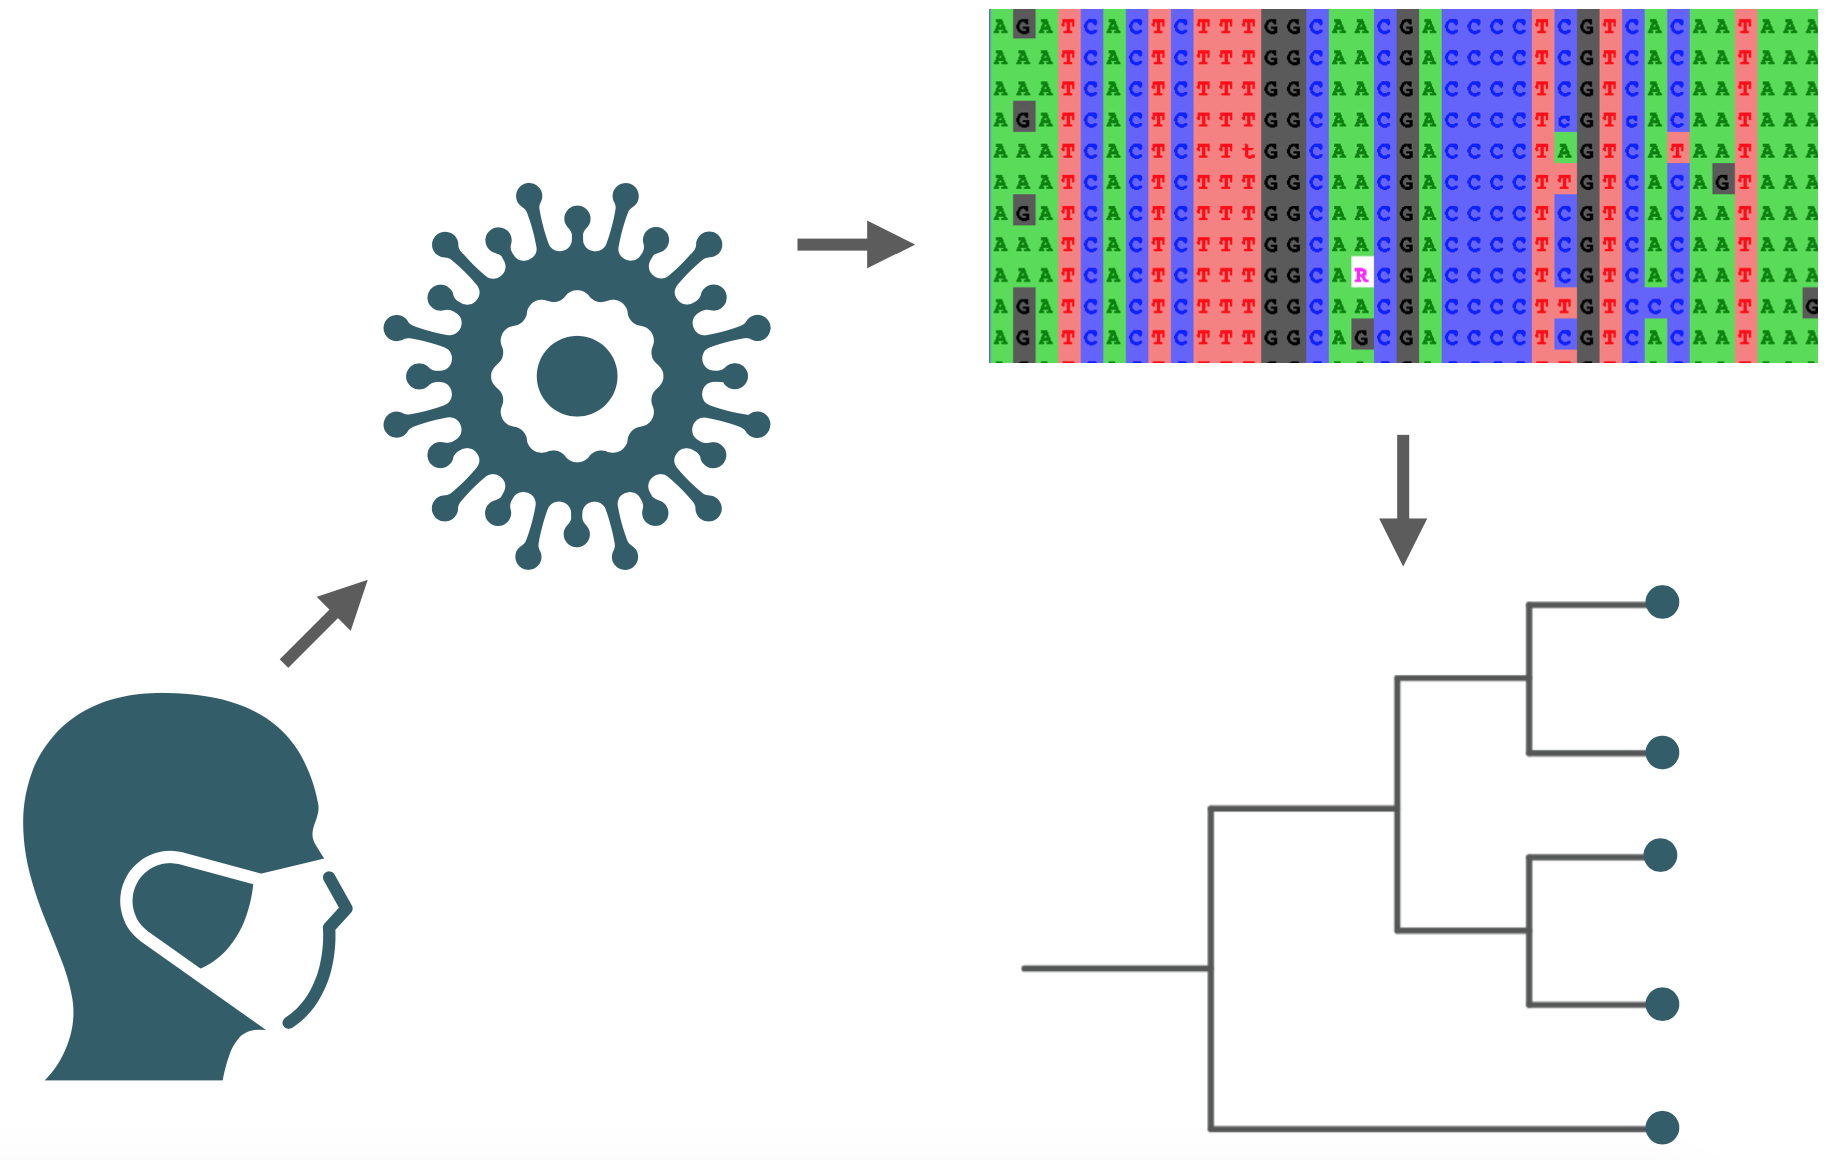
\includegraphics[width=.8\textwidth]{image/intro/phylogeny_from_sequences}
    \source{Samuel Hong (2019)}
  \end{figure}

  \note[item]{As viruses spread through the human population, they accumulate mutations in their genomes.}
  \note[item]{We can sequence these genomes and use the differences between them to hypothesize the evolutionary history that generated the observed genetic diversity. "Phylogenies"}
  \note[item]{We seek to understand the epidemiological factors that contribute to the proliferation of the virus.}

\end{frame}

%------------------------------------------------

\begin{frame}

  \frametitle{We infer geographic history from labeled phylogenies}

  \begin{figure}
    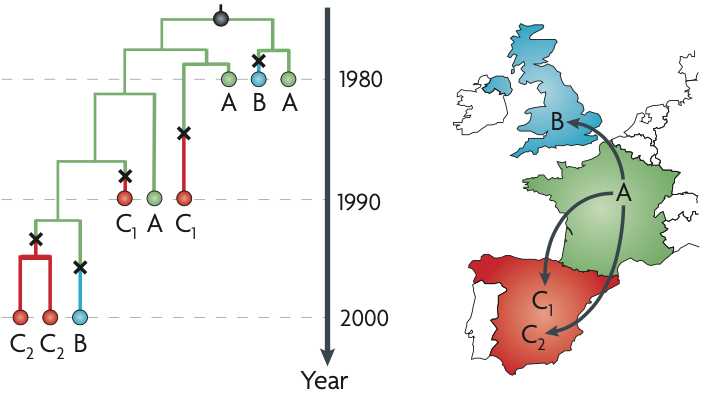
\includegraphics[width=.8\textwidth]{image/intro/phylogeography}
    \source{Pybus \& Rambaut (2009)}
  \end{figure}

  \note[item]{Interested in the spatiotemporal spread of viruses}
  \note[item]{We can do this using location data in addition to genomic data}
  \note[item]{We infer migration rates, from there we infer when the virus jumped between locations, and how many times it did}
  \note[item]{Retrospective analysis: correlate migrations with historical events}
  \note[item]{Realtime analysis: inform policy such as border closure}

\end{frame}

%------------------------------------------------

\begin{frame}

  \frametitle{We infer demographic history from phylogenies}

  \begin{figure}
    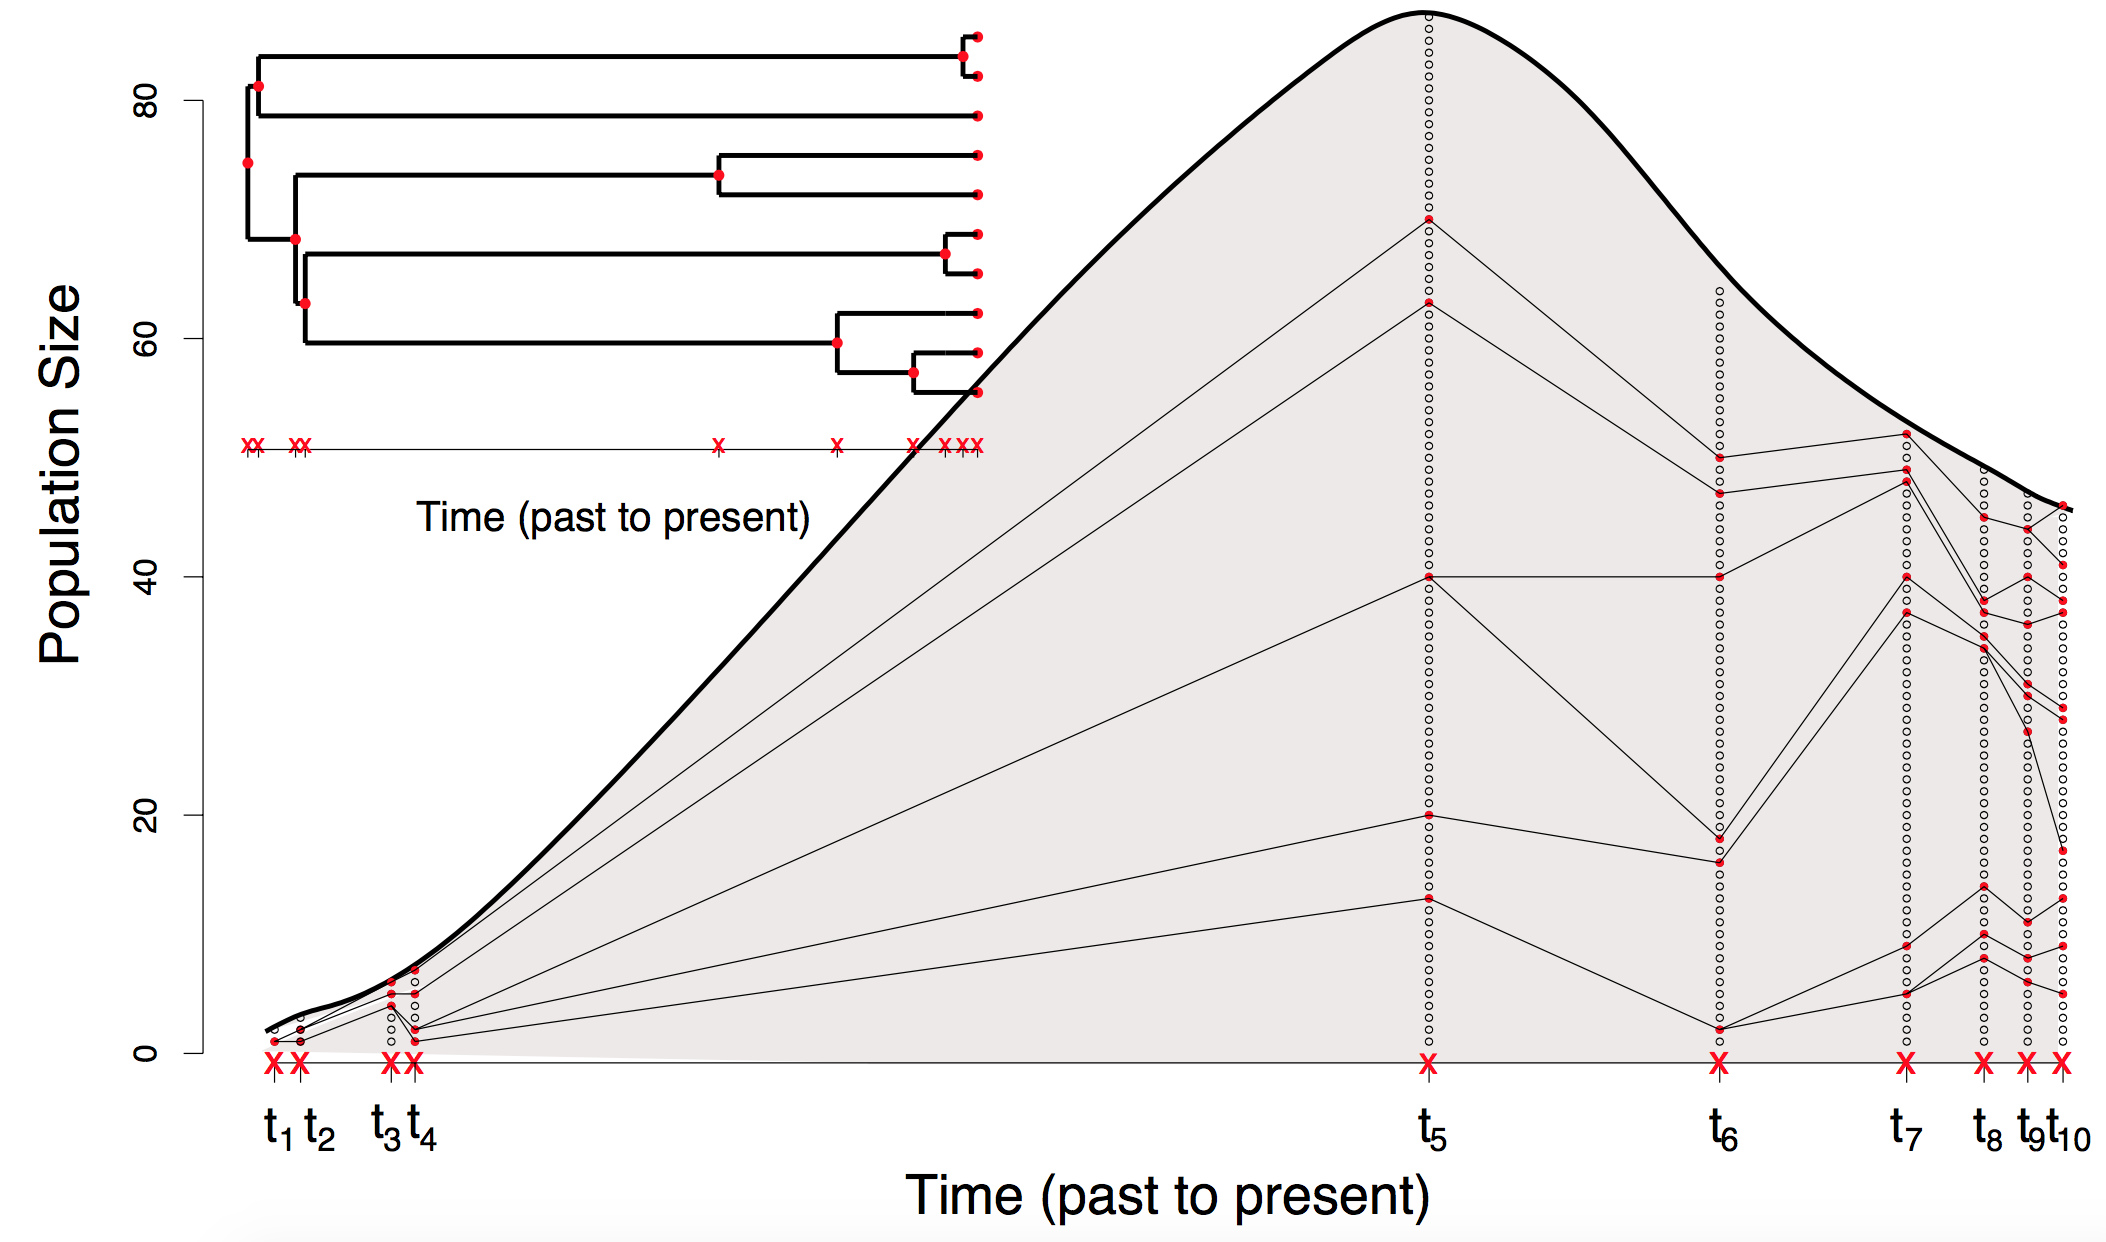
\includegraphics[width=.95\textwidth]{image/intro/skygrid1}
    \source{Palacios et al. (2014)}
  \end{figure}

  \note[item]{What do I mean by ``demographic history''?}
  \note[item]{Effective population size at different points in time}
  \note[item]{Simple models: constant population size; what is it?}
  \note[item]{Simple models: exponential population size; how quickly is it growing?}
  \note[item]{Complex models: how has the effective population size varied throughout history? What is associated with the fluctuations?}
  \note[item]{We do this by looking at branching patterns: frequency of branching is inversely proportional to population size.}

\end{frame}

%------------------------------------------------

\begin{frame}

  \frametitle{Bayesian phylogeographic inference}

  \begin{columns}[c]
    \column{0.5\textwidth}

      Given data:
      \begin{enumerate}
        \item Nucleotide sequence alignment %($S$)
        \item Sequence locations %($L$)
        \item Sampling dates %($t_{I}$)
      \end{enumerate}

    \column{.5\textwidth}
      We jointly infer:
      \begin{enumerate}
        \item Tree %($T$)
        \item Evolutionary rate
        \item Substitution rates %($\boldsymbol\mu$)
        \item Migration rates %($\boldsymbol f$)
        \item Demographic history %($\theta$)
      \end{enumerate}

  \end{columns}

  \note[item]{We are interested in figuring out the evolutionary history, the mutation rate (and different), migration rates, and the demographic history.}

\end{frame}

%------------------------------------------------

\begin{frame}

  \frametitle{Tree space is enormous}
  \begin{columns}[c]

    \column{.45\textwidth}
      Tree space size:
      $$
      \frac{(2n-3)!}{2^{n-1}(n-1)!}
      $$
    \column{.5\textwidth}
    \begin{table}
      \begin{tabular}{l l}
        \toprule
        \textbf{Taxa} & \textbf{\# of trees}\\
        \midrule
        $1$ & $1$\\
        $2$ & $1$\\
        $3$ & $3$\\
        $4$ & $15$\\
        $5$ & $105$\\
        $6$ & $945$\\
        $7$ & $10,395$\\
        $8$ & $135,135$\\
        $9$ & $2,027,025$\\
        $\vdots$ & $\vdots$\\
        $769$ & $3.753\times10^{2,110}$\\
        \bottomrule
      \end{tabular}
    \end{table}
  \end{columns}

  \note[item]{While performing Bayesian inference allows us to characterize the posterior distribution of parameters (which is nice), it is computationally intensive.}
  \note[item]{Rooted, labeled, bifurcating phylogenies.}
  \note[item]{Context: About $10^{80}$ atoms in the observable universe}
  \note[item]{Context: Universe-in-atom almost 27x}

\end{frame}

%------------------------------------------------

\begin{frame}

  \frametitle{We explore tree space using MCMC}

  \begin{figure}
    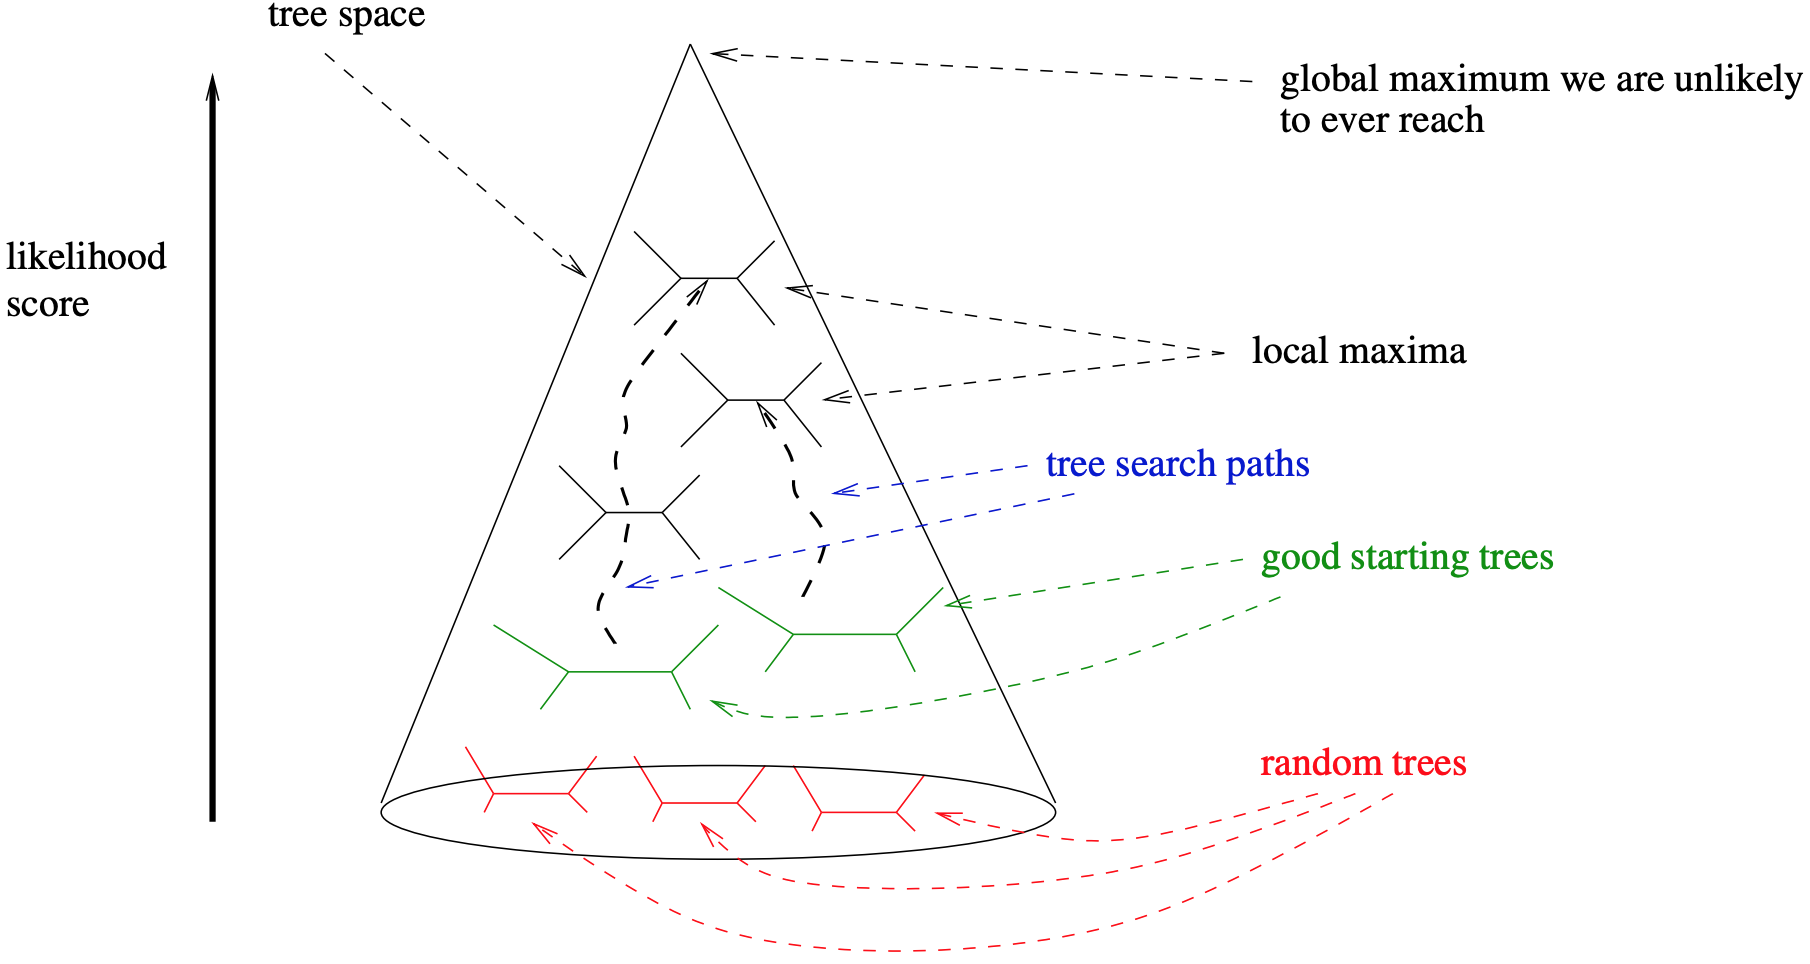
\includegraphics[width=.99\textwidth]{image/intro/tree_traversal}
    \source{Stamatakis \& Kozlov (2020)}
  \end{figure}

  \note[item]{We need a principled way to search through the enormity of state space in order to find a plausible result in a reasonable amount of time.}
  \note[item]{We do this using a type of algorithm known as MCMC}
  \note[item]{Describe figure}
  \note[item]{Once we arrive in high-likilihood space we continue to explore that region to determine the distribution of high likelihood parameters}
  \note[item]{We use a similar procedure to jointly infer the other parameters that I mentioned}

\end{frame}

%------------------------------------------------
\section{HBV phylogeography}
%------------------------------------------------

\begin{frame}

  \Large{\centerline{HBV phylogeography}}

  \note[item]{This work is currently being prepared for publication; has been handed off to co-authors}

\end{frame}

%------------------------------------------------

\begin{frame}

  \frametitle{What is HBV?}

  \begin{columns}[c] % The "c" option specifies centered vertical alignment while the "t" option is used for top vertical alignment

    \column{.45\textwidth} % Left column and width
      \begin{itemize}\itemsep=3ex
        \item Causative agent of hepatitis B; leads to cirrhosis and liver cancer
        \item Spread through blood and bodily fluids
        \item Affects $> 350$ million people annually
        \item Partially dsDNA virus
        \begin{itemize}
          \item Long strand: ~3 kb
          \item Short strand: ~2.2 kb
        \end{itemize}
      \end{itemize}

    \column{.5\textwidth} % Right column and width
      \begin{figure}
        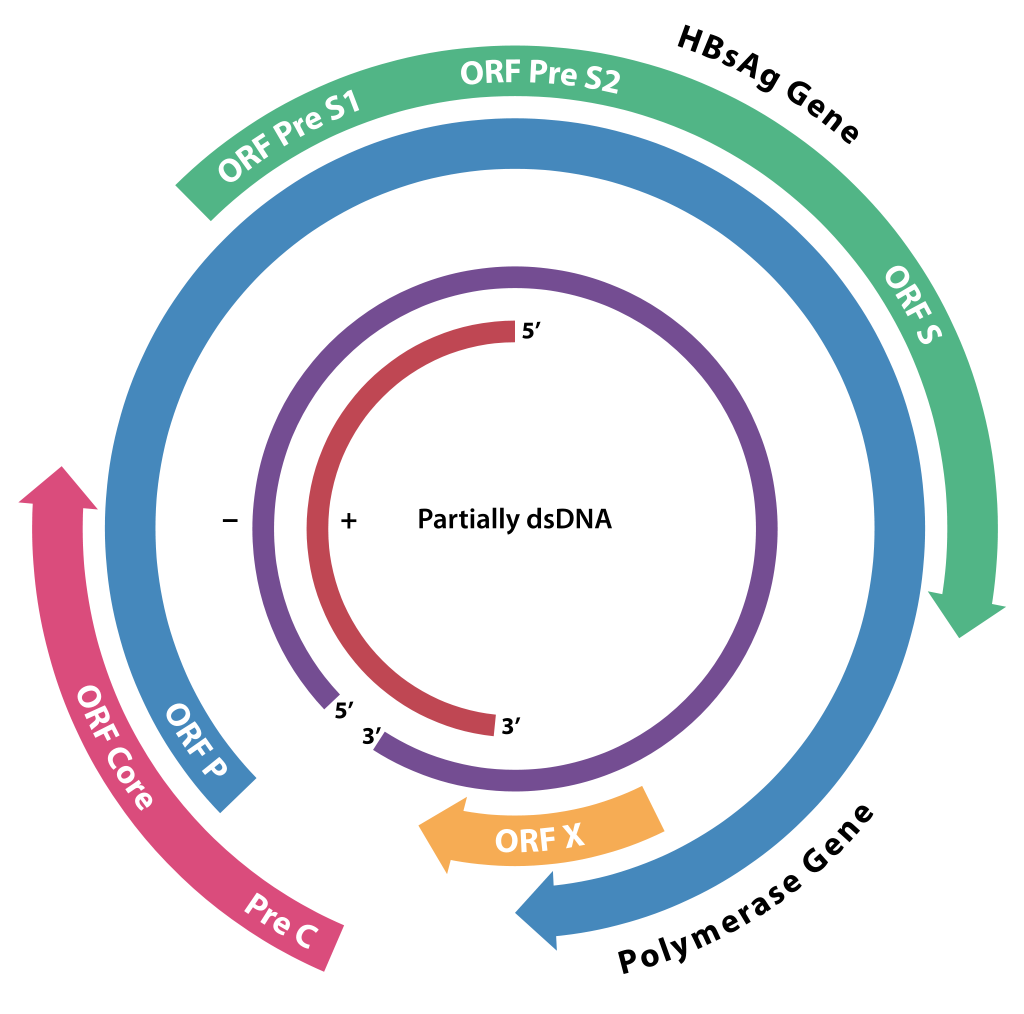
\includegraphics[width=.95\linewidth]{image/results/hbv_genome_schematic}
        \source{Wikimedia commons}
      \end{figure}

  \end{columns}

  \note[item]{HBV-A: 587, HBV-D: 769, HBV-E: 234}
  \note[item]{Our new sequences: 145 novel strains}
  \note[item]{Sequenced from samples taken from patients who had recently immigrated to Belgium from Africa}

\end{frame}

%------------------------------------------------

\begin{frame}

  \frametitle{Objectives}

  Reconstruct evolutionary and migration history of three HBV genotypes (A, D, E):
  \vfill
  \begin{itemize}\itemsep=3ex
    \item When was the most recent common ancestor of each HBV genotype?
    \item When were the major migrations of each genotype; do these migrations correspond with known human movements?
    \item How many times did each genotype move between regions?
  \end{itemize}
\end{frame}


%------------------------------------------------

\begin{frame}

  \frametitle{HBV presents three major challenges}

  \begin{enumerate}\itemsep=3ex
    \item Large datasets of up to 769 taxa cause lengthy ($\geq 1$ month) computation times
    \item Rampant sampling bias makes accurate geographic inference difficult
    \item HBV demonstrates minimal temporal signal
  \end{enumerate}

\end{frame}

%------------------------------------------------

\begin{frame}

  \frametitle{Dataset size prevents easy computation}
  \begin{figure}
    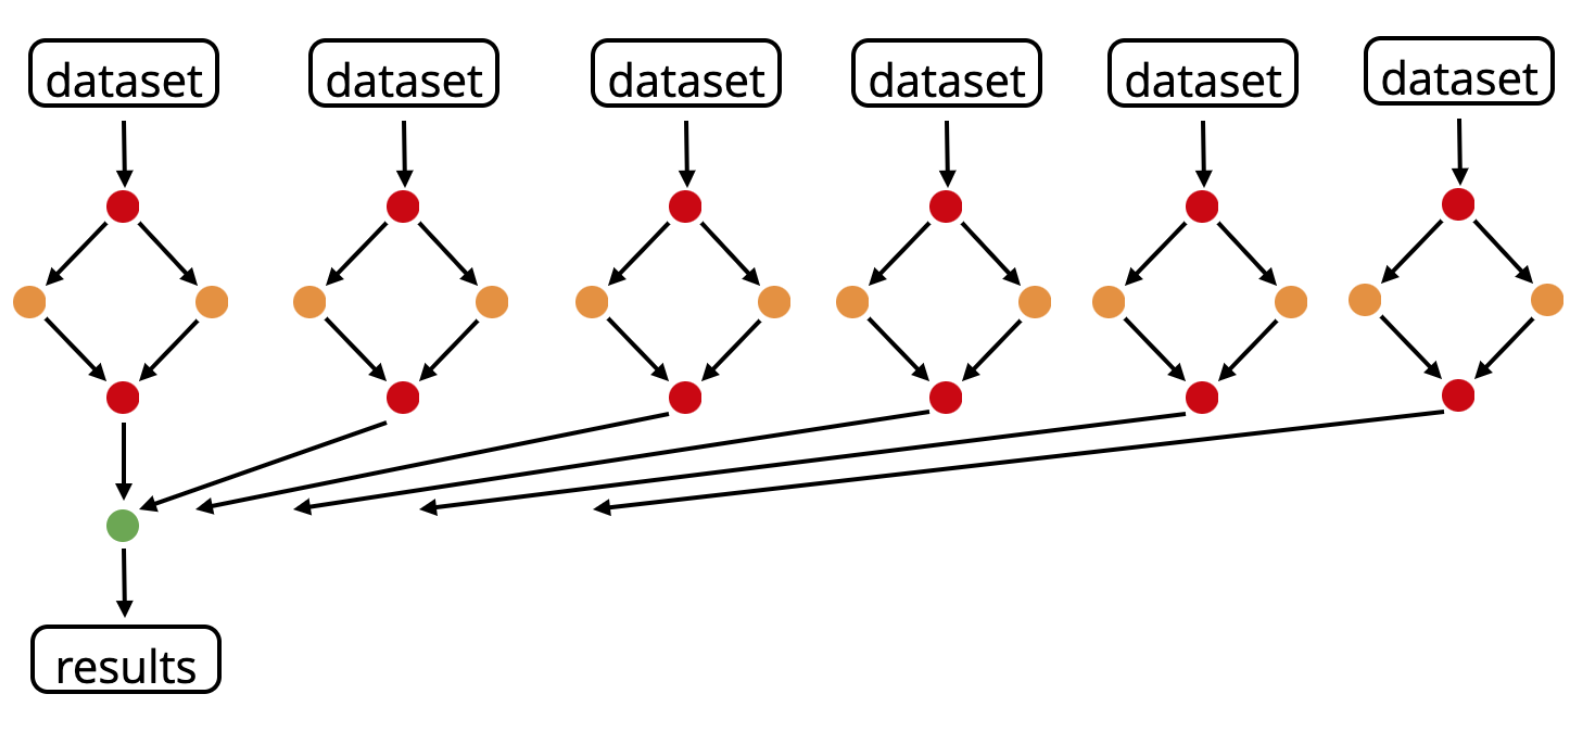
\includegraphics[width=.95\linewidth]{image/methods/parallel_builds}
    \source{Johannes K\"{o}ster (2019)}
  \end{figure}

  \note[item]{We circumvent computation time issues by parallelizing computational replicates of the same dataset; aggregate our results at the end}
  \note[item]{Added bonus: because we are randomly exploring state space, if we arrive at the same result from different starting points we are more confident in our results}

\end{frame}

%------------------------------------------------

\begin{frame}

  \frametitle{Dataset size prevents easy computation}

  \begin{itemize}\itemsep=3ex
    \item We are interested in accumulating independent samples through MCMC procedure
    \item Joint inference of geographic history significantly slows computational speed
    \item We circumvent computational issues by conditioning geographic inference on phylogenetic results
  \end{itemize}

  \note[item]{DTA scales cubically with number of states}

\end{frame}

%------------------------------------------------

\begin{frame}

  \frametitle{Sampling bias complicates phylogeographic inference}

  \begin{figure}
    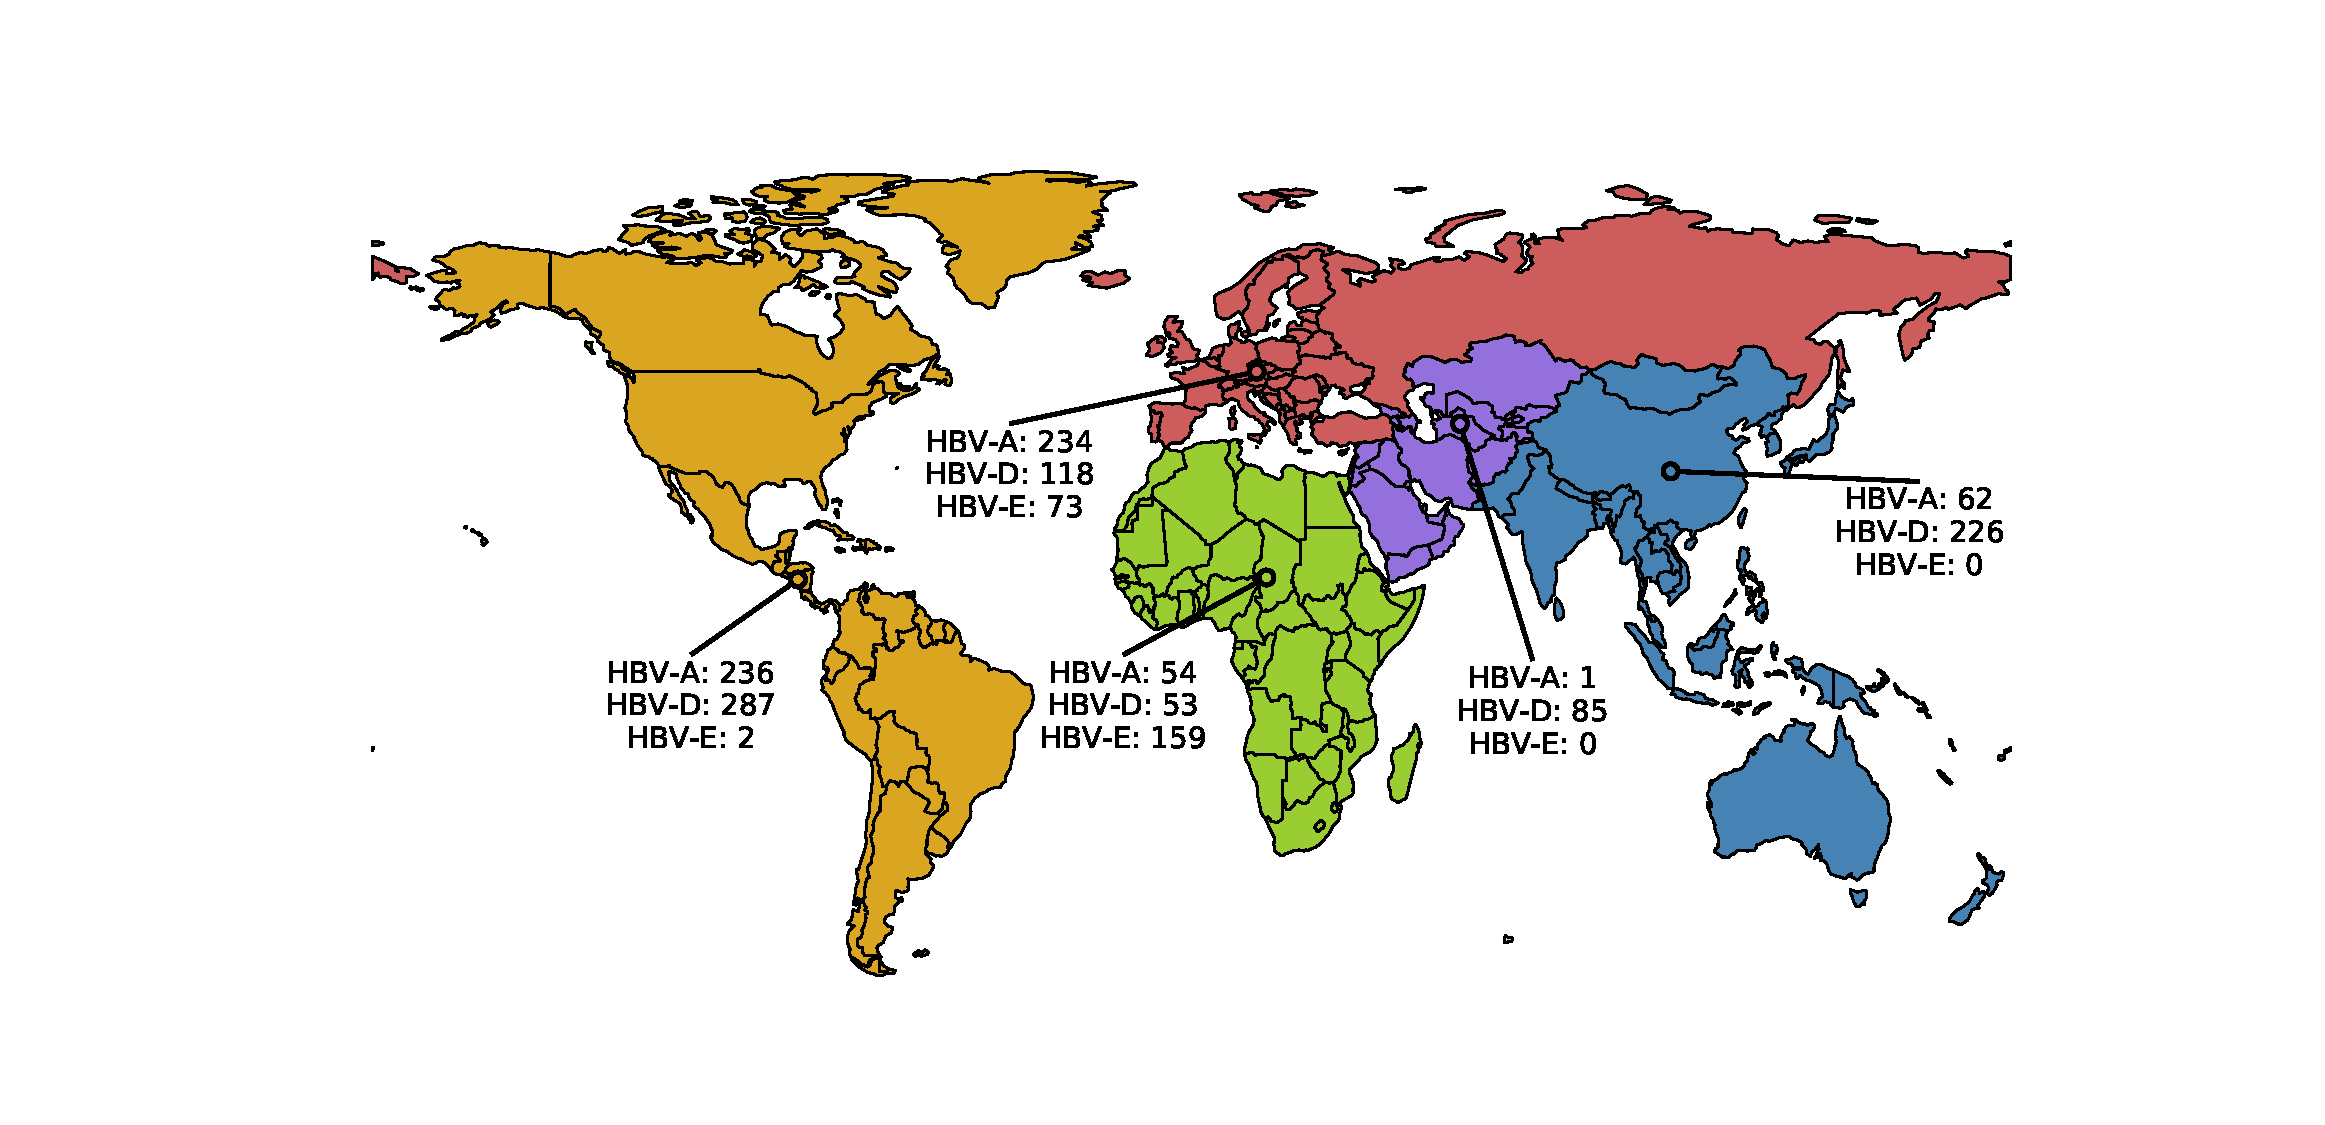
\includegraphics[width=\linewidth]{image/methods/static_map_with_counts}
  \end{figure}

  \note[item]{Sampling bias can have a huge affect on our geographic inference: over represented regions dominate the results}
  \note[item]{54 countries represented in our dataset; 165 Iran HBV-D, 13 singletons, 37 instances of fewer than 5 sequences for a country}
  \note[item]{Splitting by country we have a few massively represented countries, and many singletons}
  \note[item]{Splitting by continent we see some similar issues}
  \note[item]{We chose these five regions to create the most equitable split among regions that are representative of large-scale historical human movement patterns}
  \note[item]{Bonus: computational time is significantly increased by an increased number of geographic bins}

\end{frame}

%------------------------------------------------

\begin{frame}

  \frametitle{HBV lacks temporal signal}

  \begin{figure}
    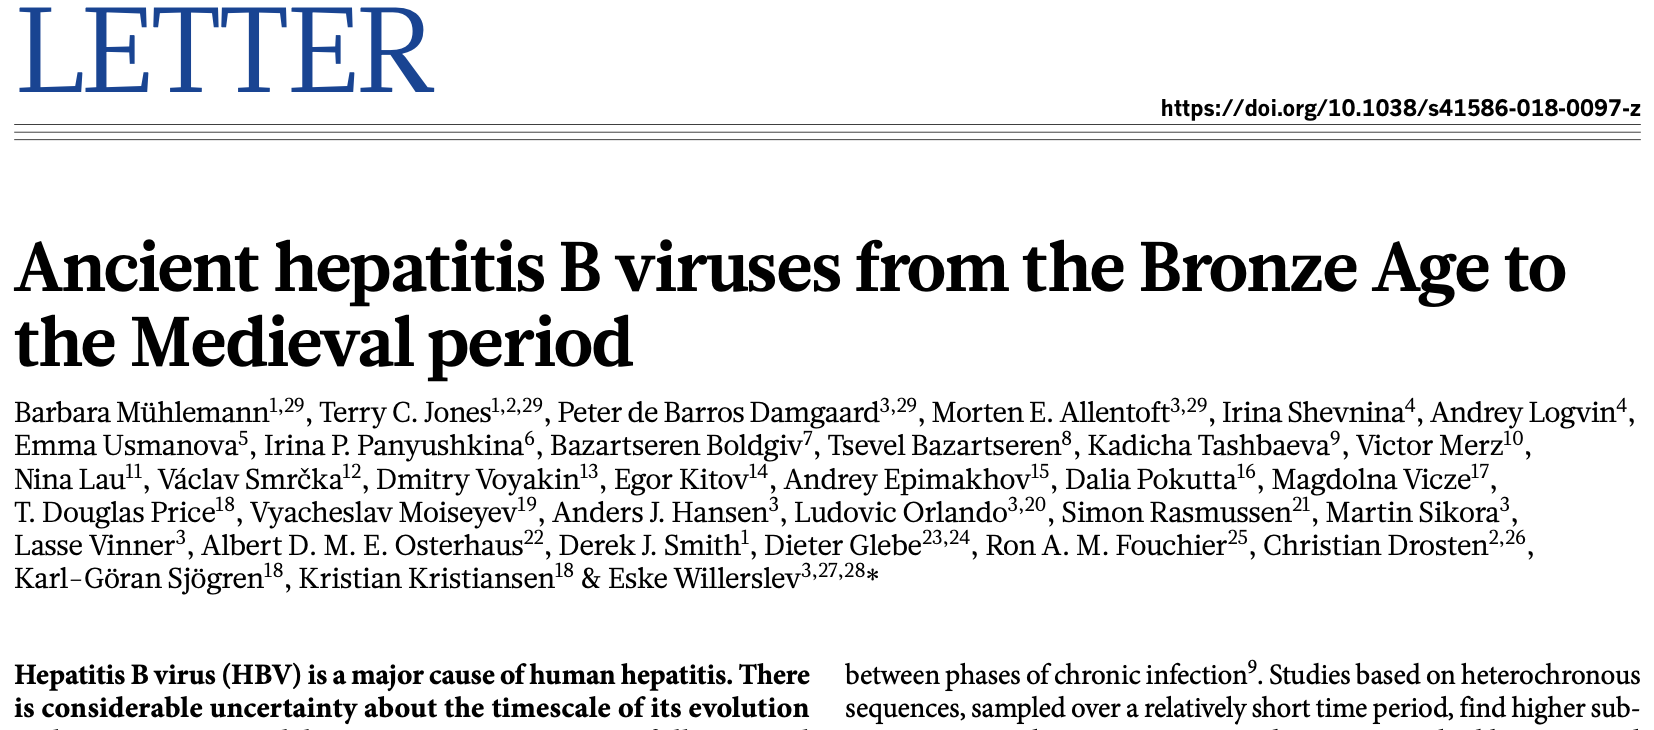
\includegraphics[width=.95\linewidth]{image/methods/muhlemann}
  \end{figure}

  \note[item]{To date internal nodes of the tree we need some way to relate genetic distance to time}
  \note[item]{We leverage the ``clock-like'' nature of mutation accumulation over time, along with samples taken serially through time to create this correlation}
  \note[item]{Without other means to calibrate internal nodes, we need rapidly-evolving viruses or access to ancient sequences}

\end{frame}

%------------------------------------------------

\begin{frame}
  \frametitle{Ancient genomes provide temporal signal}
  \begin{table}
    \begin{tabular}{l l l l}
    \toprule
    \textbf{Sequence} & \textbf{Genotype} & \textbf{Location} & \textbf{Age (year)}\\
    \midrule
    Rise386 & HBV-A & Russia$^*$ & 4,114 (2100 BCE)\\
    Rise387 & HBV-A & Russia$^*$ & 4,278 (2264 BCE)\\
    DA119 & HBV-A & Slovakia & 1,563 (451 CE)\\
    DA195 & HBV-A & Hungary & 2,641 (627 BCE)\\
    \midrule
    DA27 & HBV-D & Kazakhstan & 1,610 (409 CE)\\
    DA29 & HBV-D & Kazakhstan & 822 (1197 CE)\\
    DA51 & HBV-D & Kyrgyzstan & 2,297 (278 BCE)\\
    DA222 & HBV-D & Kazakhstan & 1,167 (852 CE)\\
    NASD24SEQ & HBV-D & Italy & 427 (1587 CE)\\
    \bottomrule
    \end{tabular}
    \source{Muhlemann et al. (2018), Ross~et~al.~(2018)}
  \end{table}

  Clock rate prior: $1.18 \times 10^{-5}$ [95\% HPD: $8.04 \times 10^{-6} \textrm{--} 1.51 \times 10^{-5}$] subs./site/year

  \note[item]{We have new sequences for HBV-A and HBV-D}
  \note[item]{Russian sequences are actually classified as Central Asian (near border with Kazakhstan)}
  \note[item]{Italian sequence comes from Ross et al. (2018)}
  \note[item]{We get a Lognormal evolutionary rate prior from the Muhlemann paper}

\end{frame}

%------------------------------------------------

\begin{frame}

  \frametitle{HBV-A phylogeography}

  \begin{figure}
    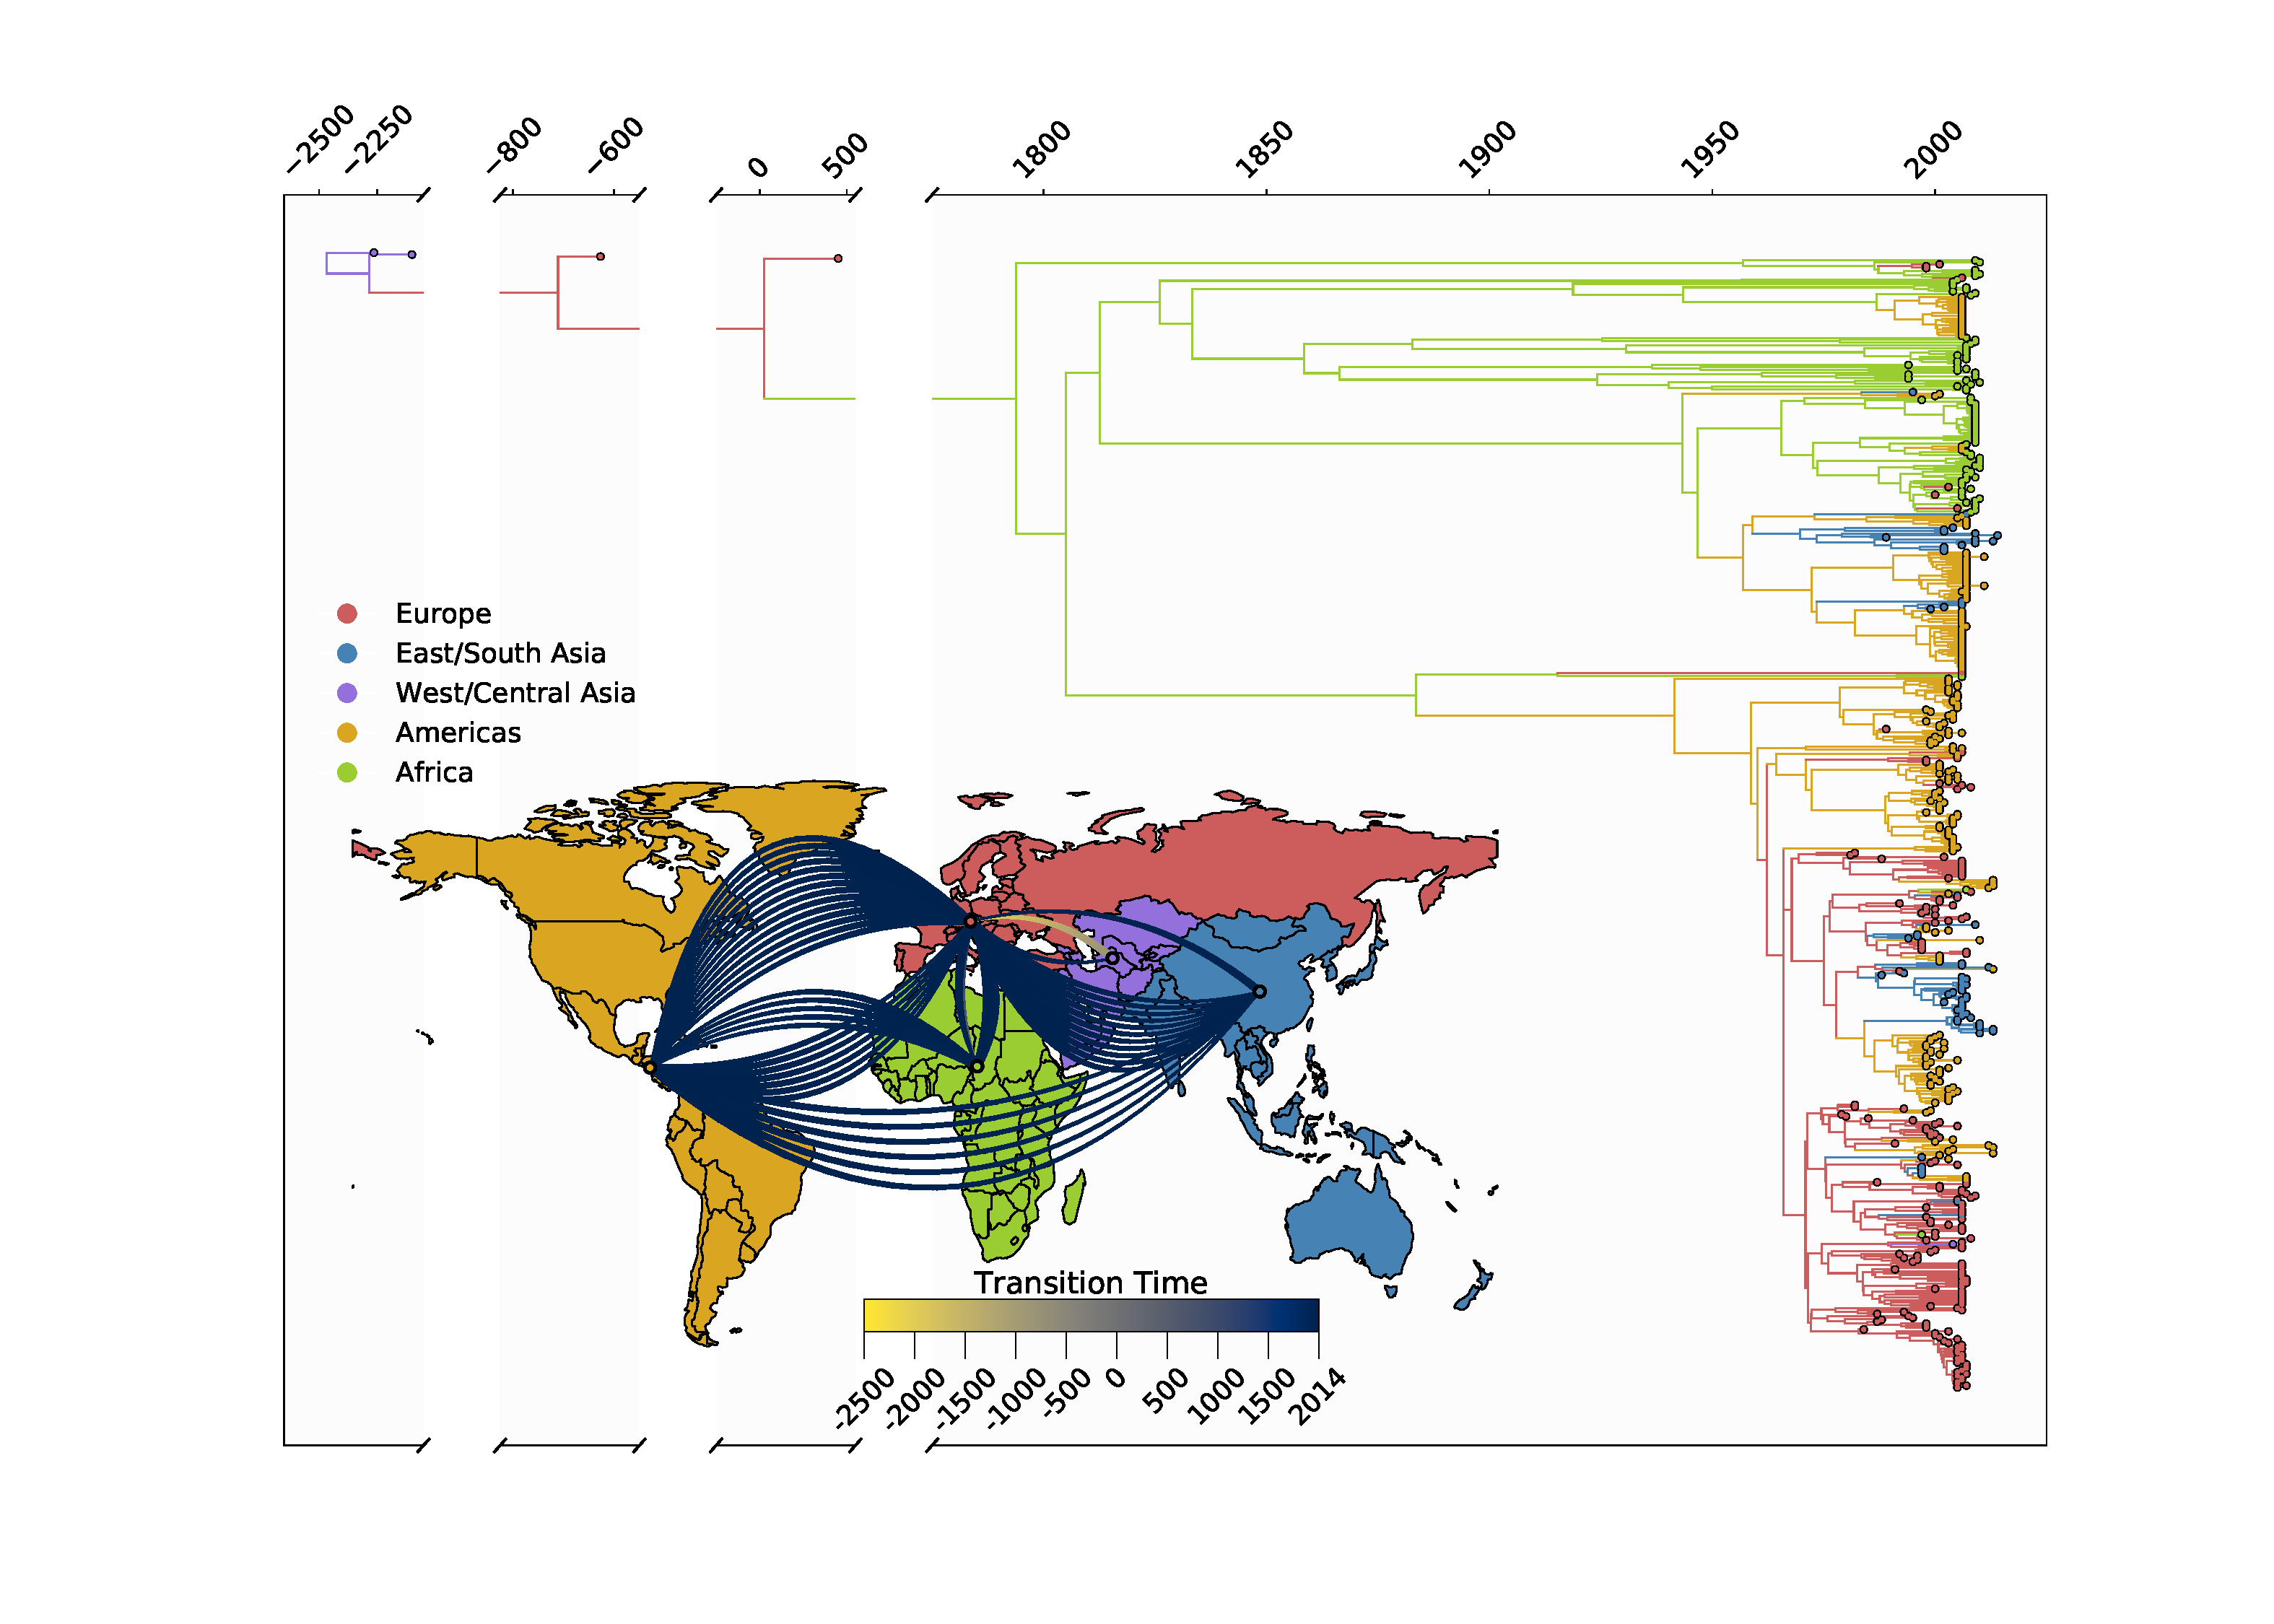
\includegraphics[width=.9\linewidth]{image/results/HBV-A_phylogeography_and_mcc_tree}
  \end{figure}

  \note[item]{Explain figure}
  \note[item]{Maximum clade credibility tree with map}
  \note[item]{tMRCA is around 2500 BCE}
  \note[item]{Ancestral location is informed by ancient sequences, so we can't be sure that it is totally accurate}

\end{frame}

%------------------------------------------------

\begin{frame}

  \frametitle{HBV-A phylogeography}

  \begin{figure}
    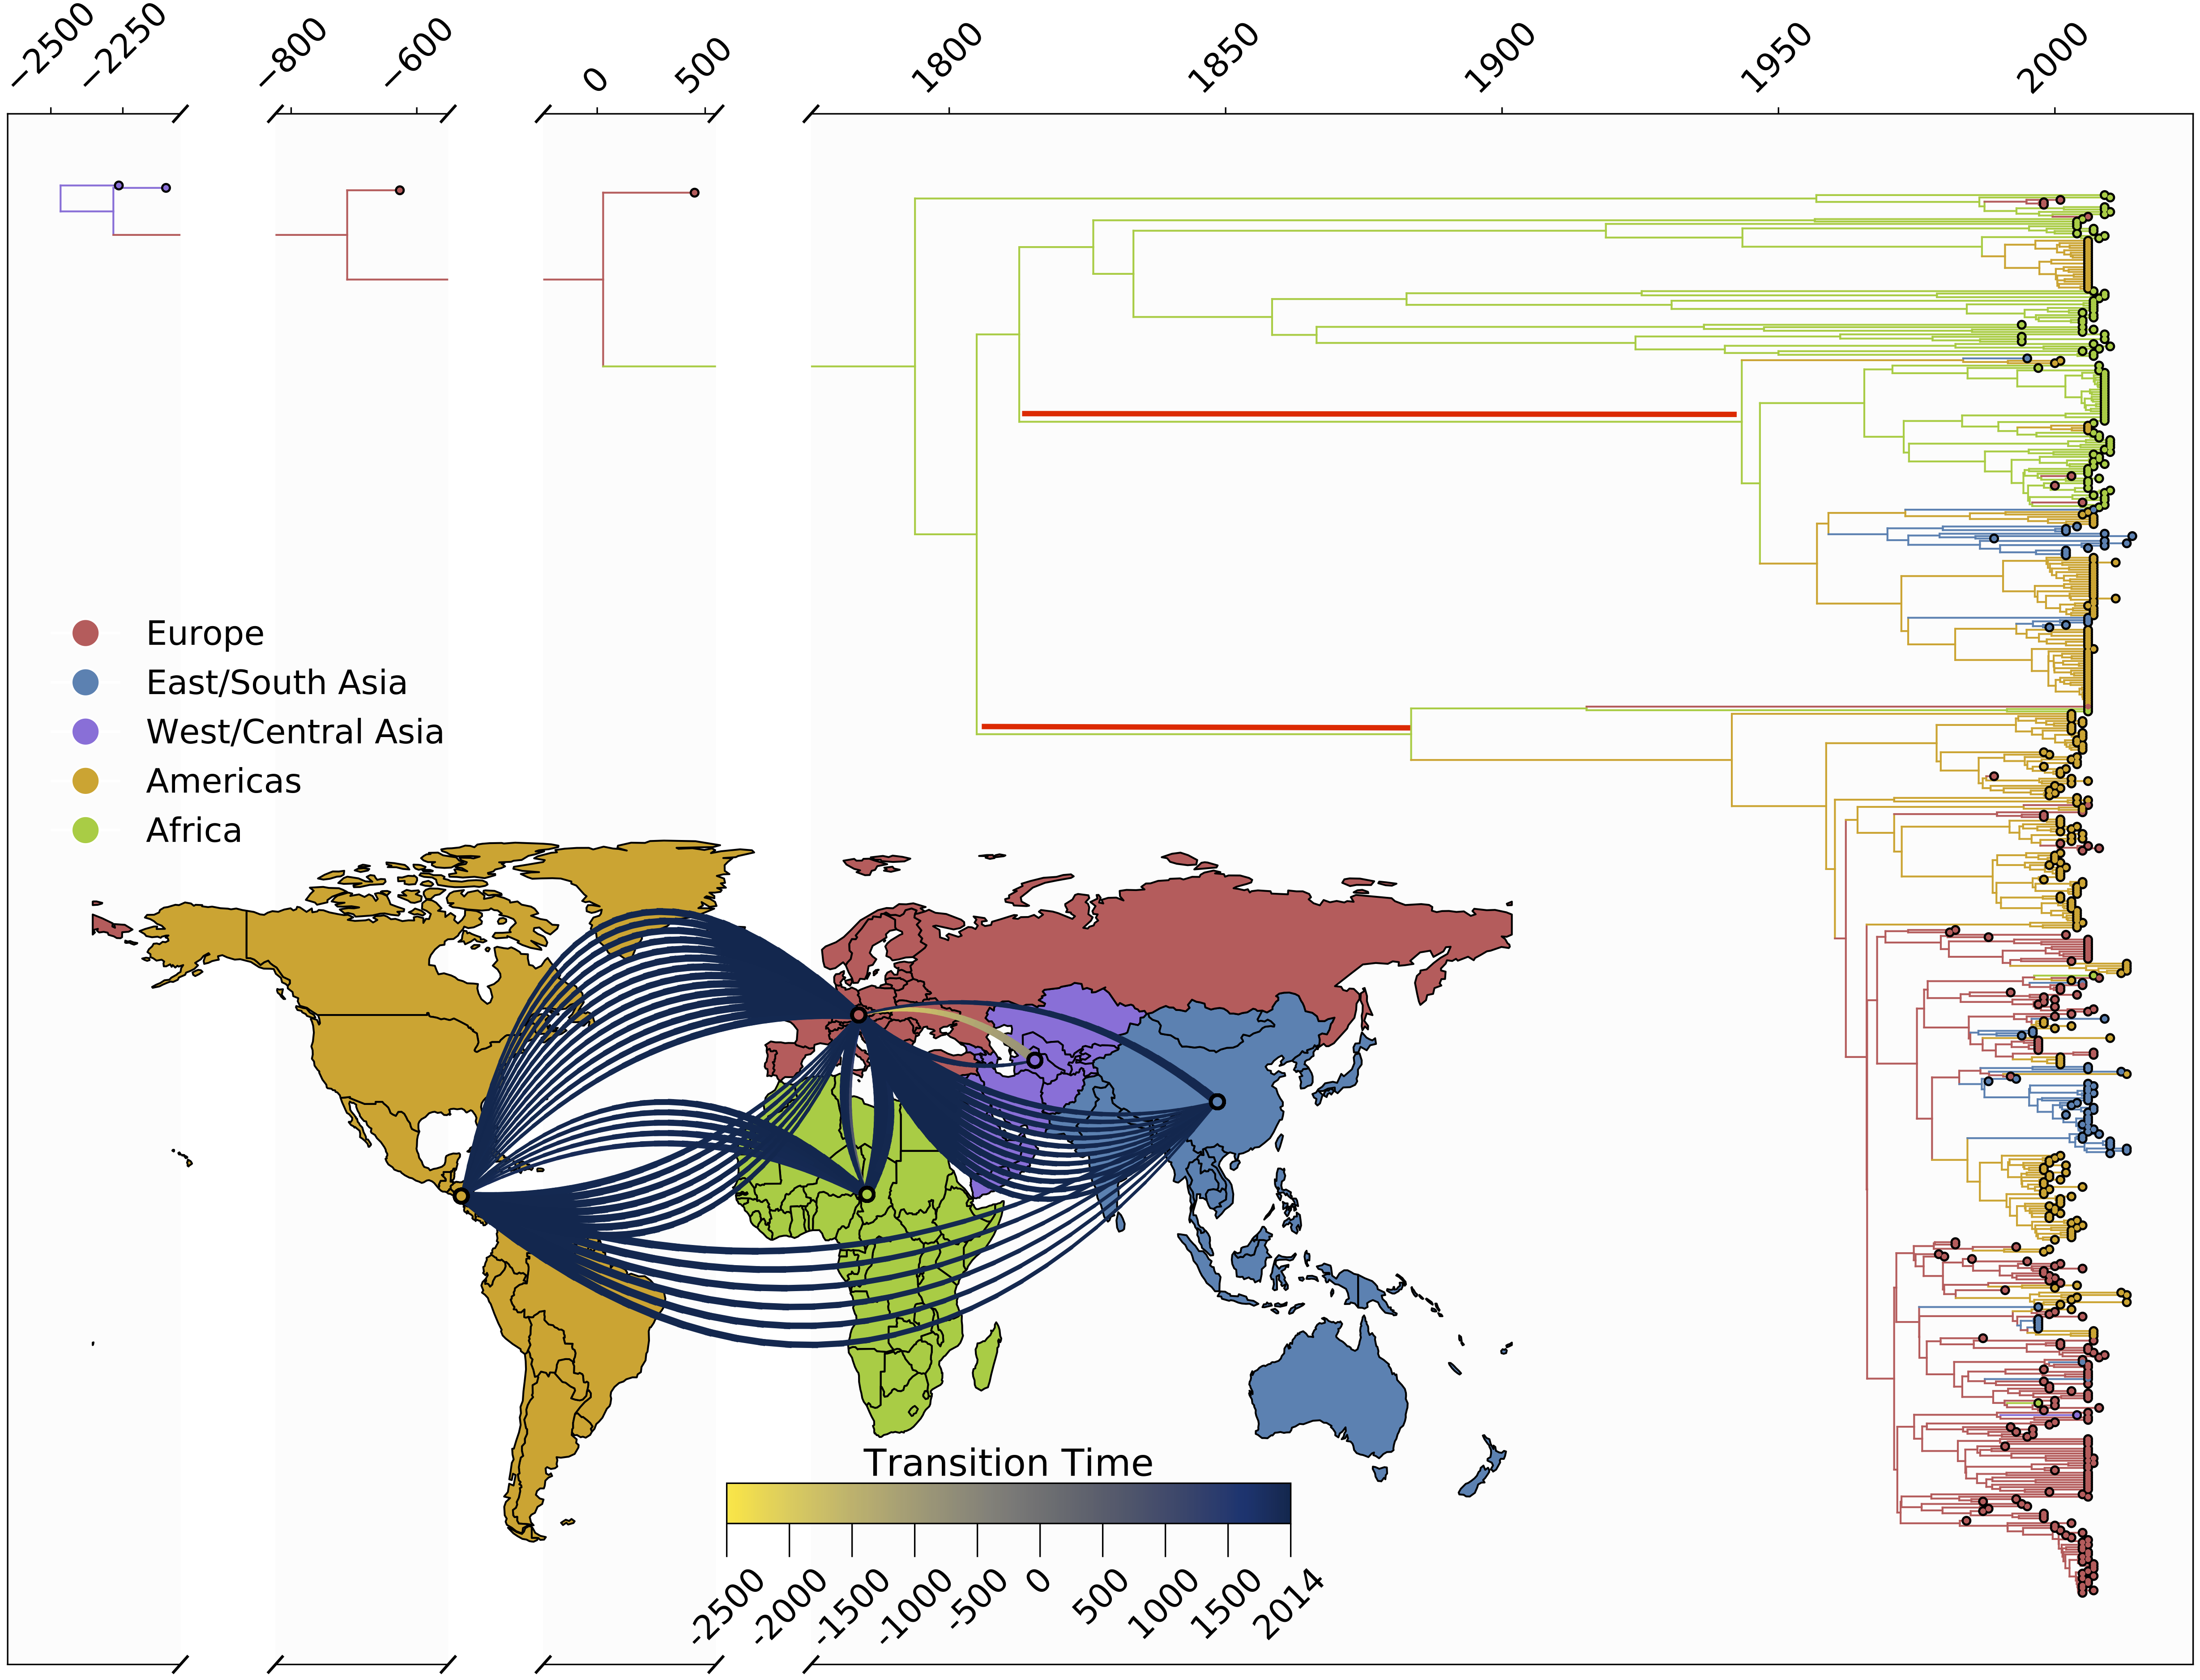
\includegraphics[width=.9\linewidth]{image/results/HBV-A_phylogeography_and_mcc_tree_with_highlights.png}
  \end{figure}

  \note[item]{A few branches are inferred to have existed in Africa, however they have many children in the Americas; their timing overlaps with the end of the Atlantic Slave Trade}
  \note[item]{Atl. Slave Trade formally ended in the US in 1808; continued to 1860 in South/Central America}

\end{frame}

%------------------------------------------------

\begin{frame}

  \frametitle{HBV-A phylogeography}

  \begin{figure}
    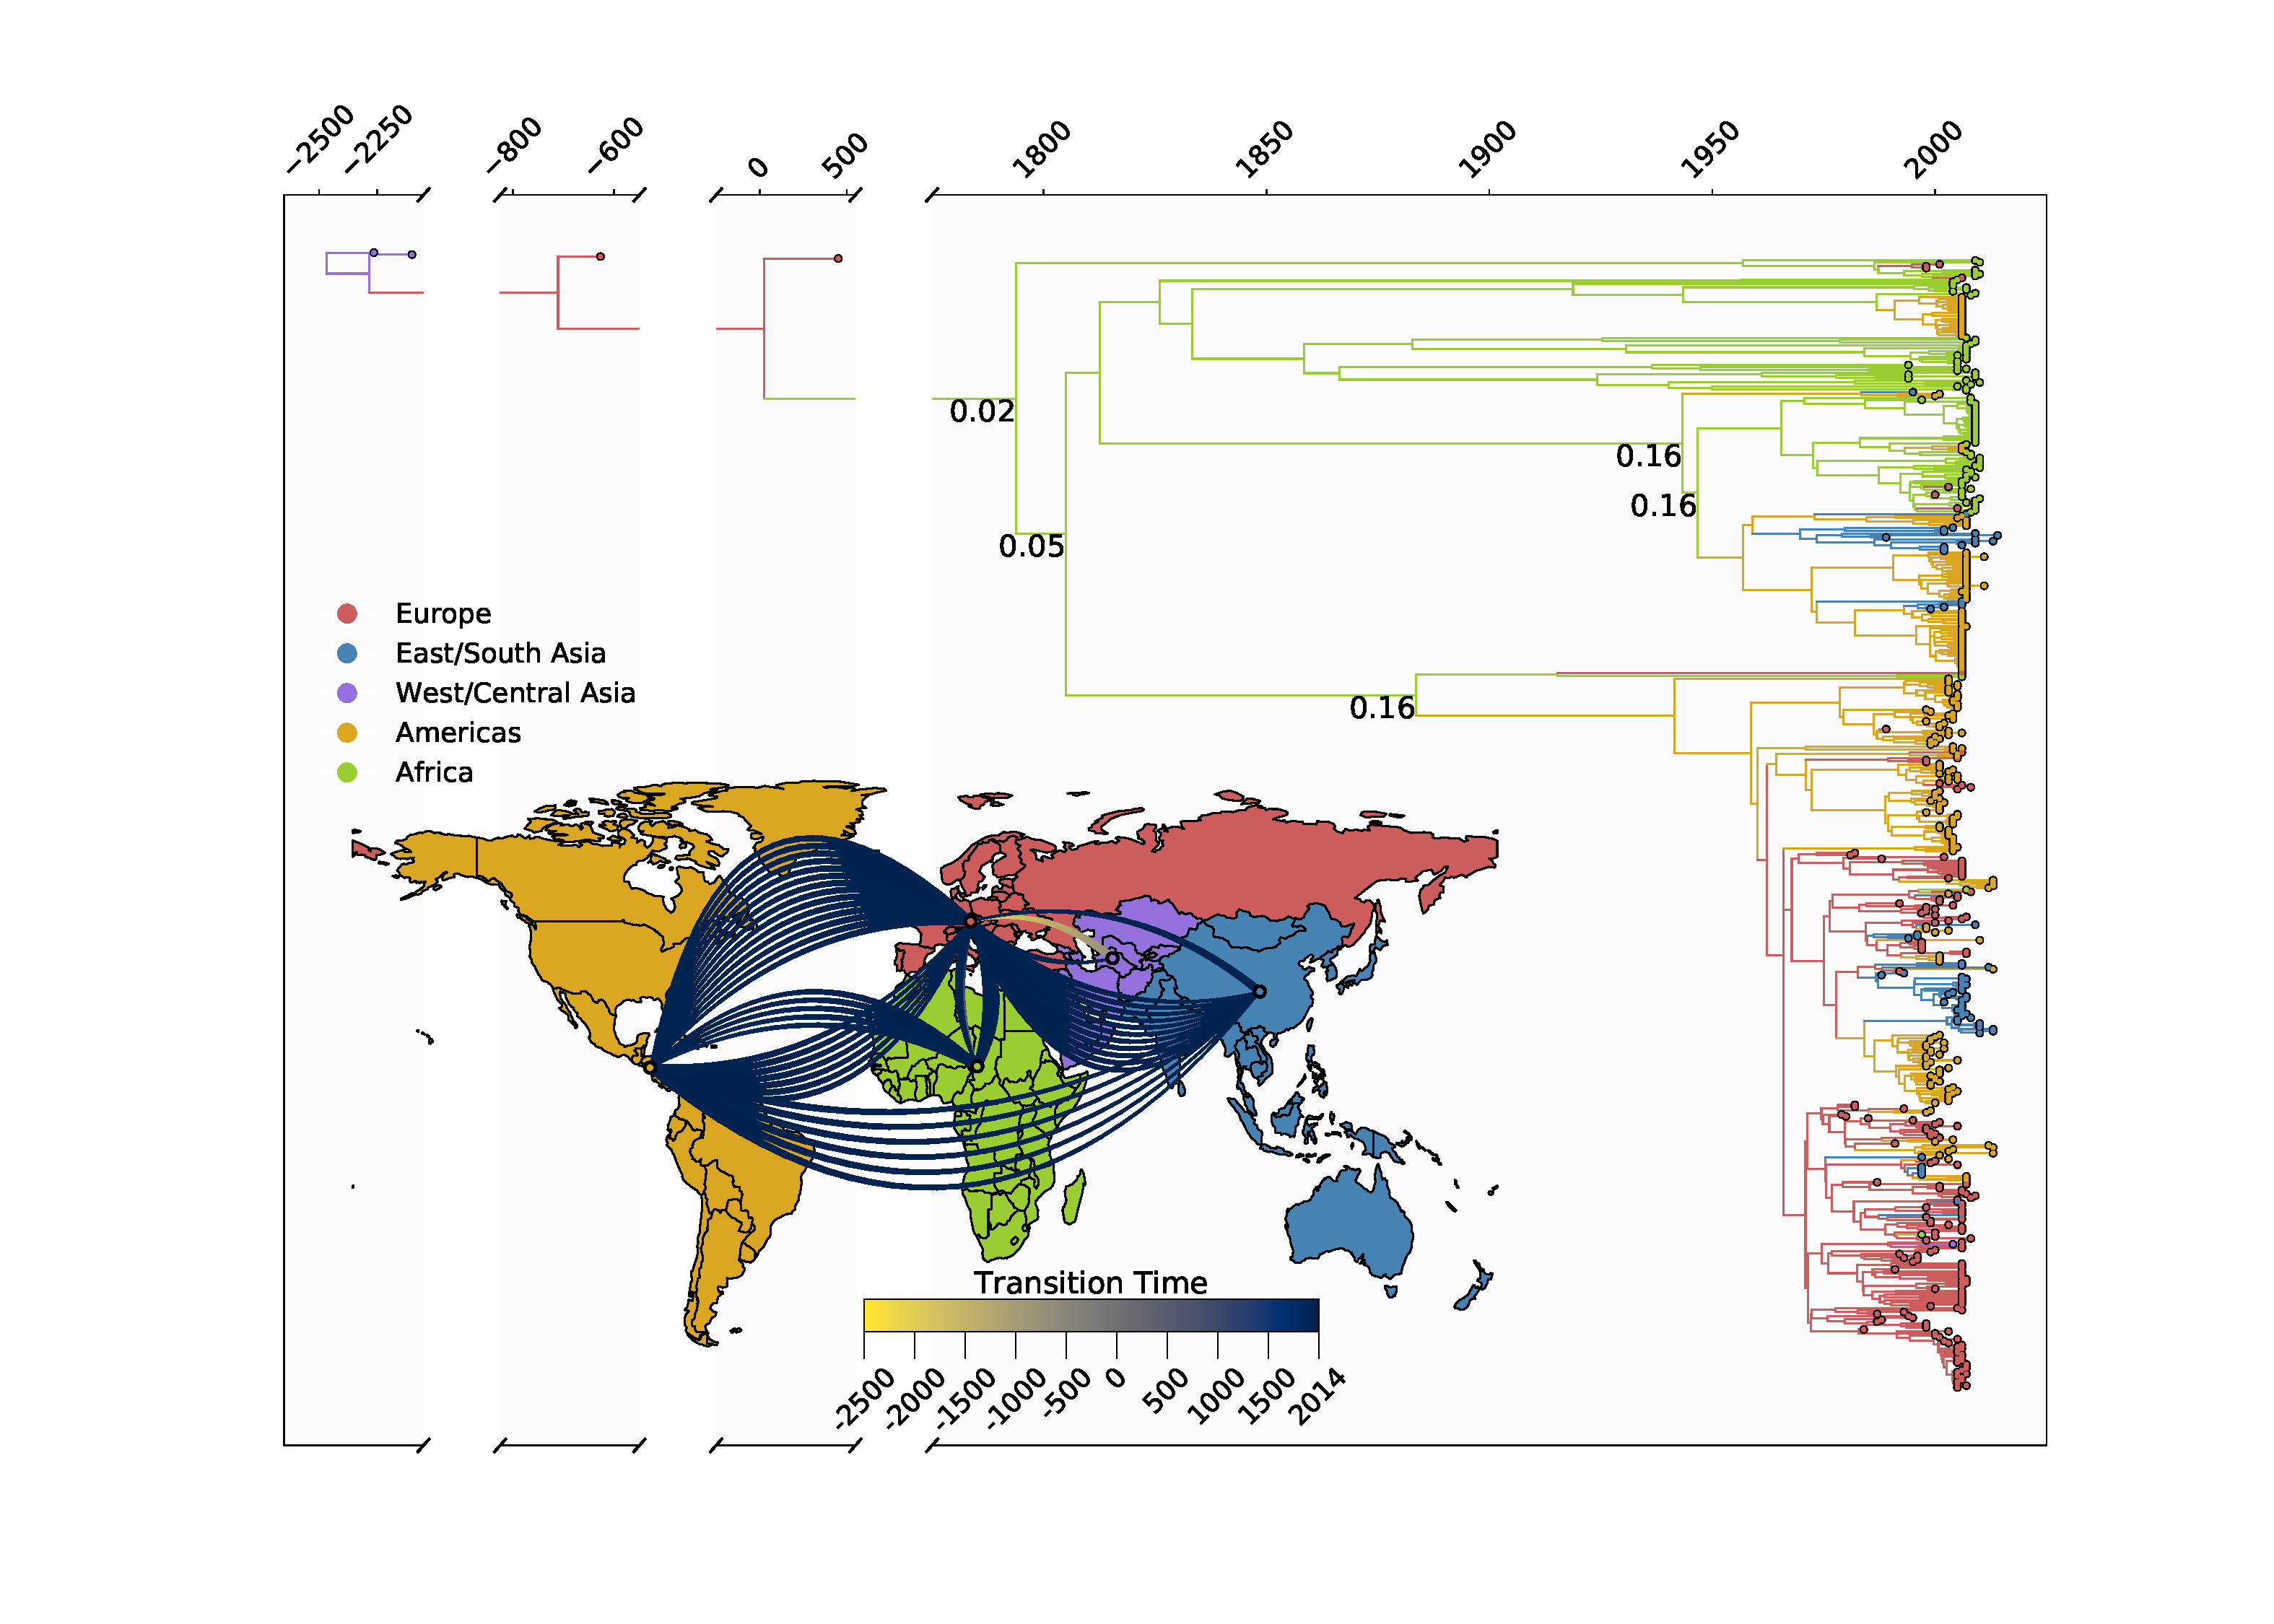
\includegraphics[width=.9\linewidth]{image/results/HBV-A_phylogeography_and_mcc_tree_annotated}
  \end{figure}

  \note[item]{Calculated the probability that each branch was in the Americas (greater than 1\% shown)}
  \note[item]{The chance of that is relatively unlikely, given the results of our discrete trait analysis}

\end{frame}

%------------------------------------------------

\begin{frame}

  \frametitle{HBV-D phylogeography}

  \begin{figure}
    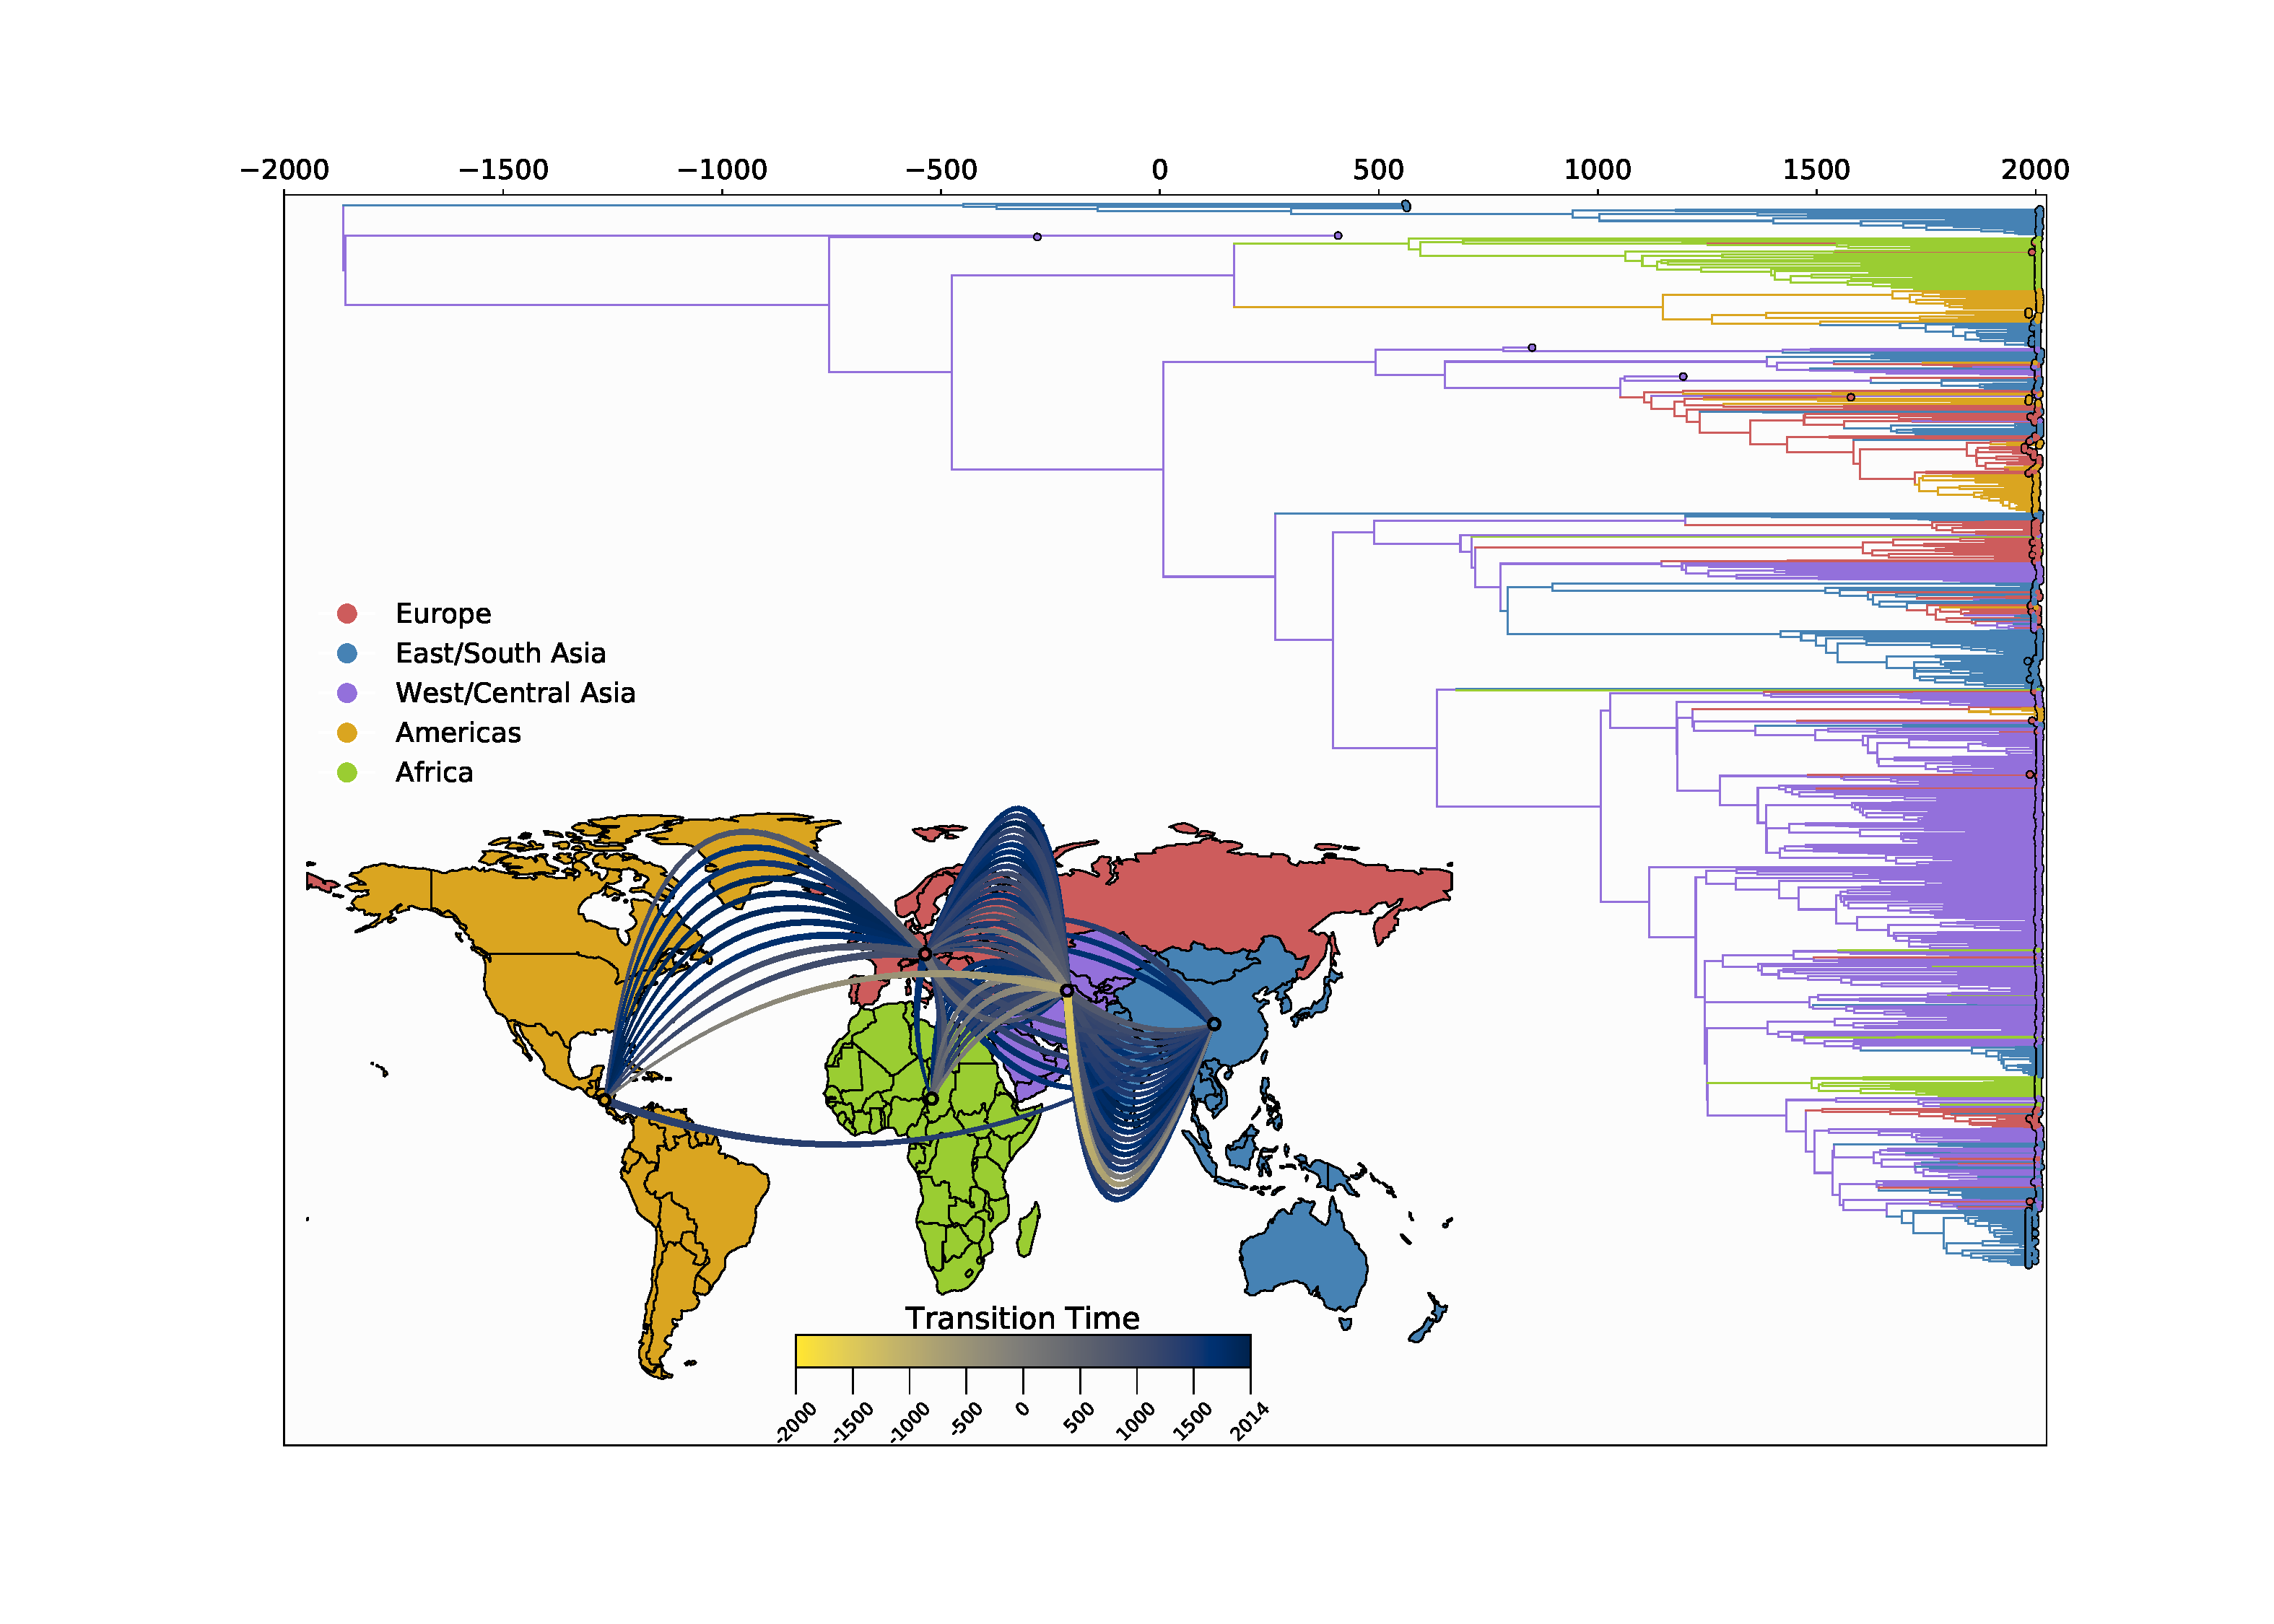
\includegraphics[width=.95\linewidth]{image/results/HBV-D_phylogeography_and_mcc_tree}
  \end{figure}

  \note[item]{Backbone of the tree is in Central Asia}
  \note[item]{tMRCA is roughly 1800 BCE}
  \note[item]{We see jumps into other regions; lots of persistent jumps, many one-offs as well}
  \note[item]{Time scale is potentially pretty messed up}

\end{frame}

%------------------------------------------------

\begin{frame}

  \frametitle{HBV-E phylogeography}

  \begin{figure}
    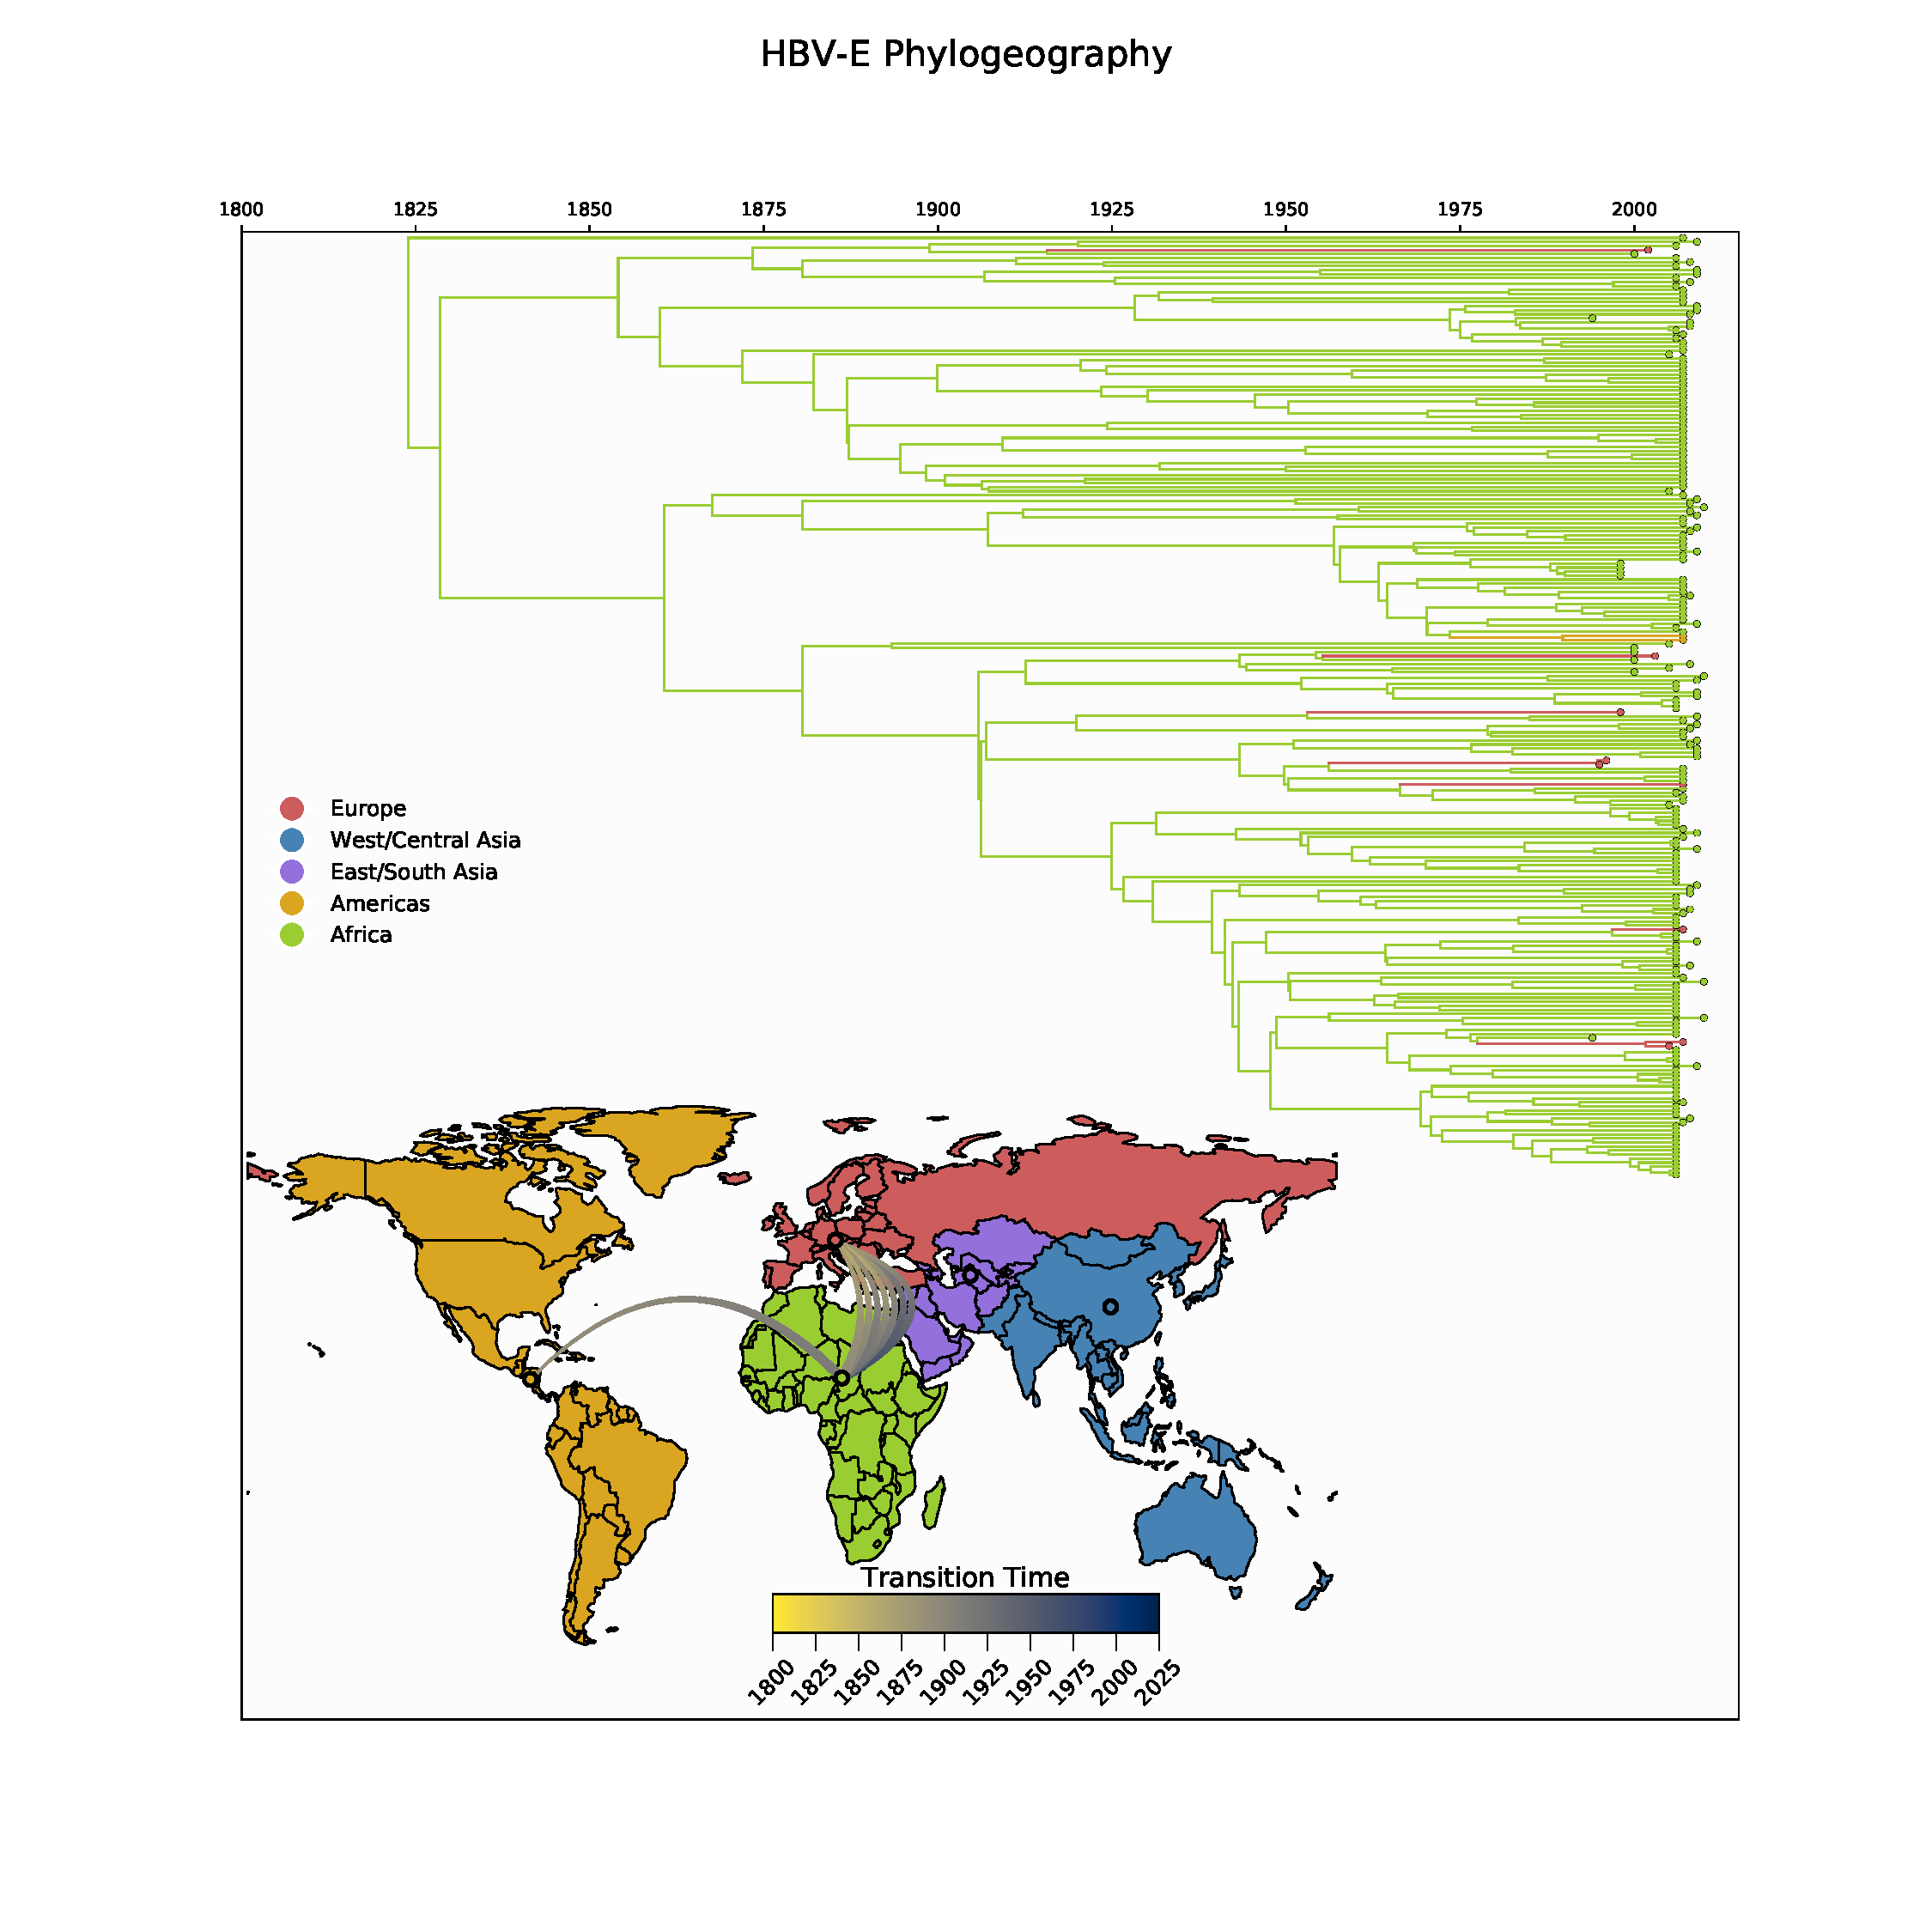
\includegraphics[width=.95\linewidth]{image/results/HBV-E_phylogeography_and_mcc_tree}
  \end{figure}

  \note[item]{tMRCA is 1824 CE}
  \note[item]{Almost all sequences come from Africa, therefore it dominates the geographic history}
  \note[item]{One-off introductions to Europe and the Americas}
  \note[item]{Roughly half of these sequences are the ones we introduce (i.e. African introductions to Belgium)}

\end{frame}

%------------------------------------------------

\begin{frame}

  \frametitle{Next steps}

  \begin{itemize}\itemsep=3ex
    \item Increase accuracy of phylogeographic inference through joint inference
    \item Make more refined geographic estimates through other methods of phylogeographic modeling
    \item Further reduce sampling bias by gathering more sequences from under represented regions
  \end{itemize}

  \note[item]{Consider structured coalescent analysis}
  \note[item]{Try to increase temporal signal to make sure historical dates are correct}
  \note[item]{Consider scraping databases for more samples to fill out spatiotemporal spread of our dataset}

\end{frame}

%------------------------------------------------
\section{LASV phylogenetics}
%------------------------------------------------

\begin{frame}

  \Large{\centerline{Lassa phylogenetics}}

  \note[item]{This project is more methodological}

\end{frame}

%------------------------------------------------

\begin{frame}

  \frametitle{What is Lassa virus?}

  \begin{figure}
    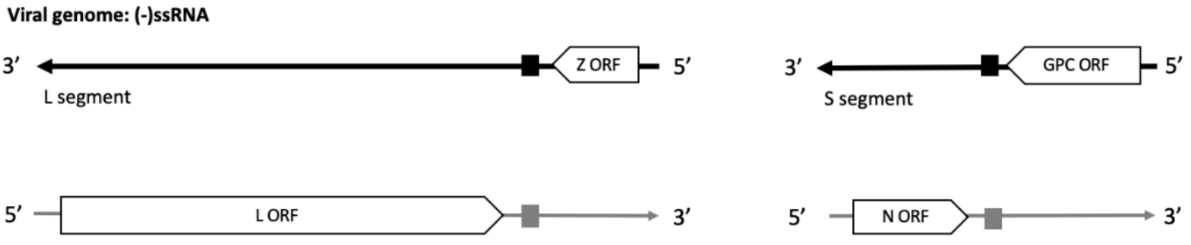
\includegraphics[width=.95\linewidth]{image/intro/lassa_genome_schematic}
    \source{Kafetzopoulou (2019)}
\end{figure}

  \begin{columns}[c] % The "c" option specifies centered vertical alignment while the "t" option is used for top vertical alignment

    \column{.45\textwidth} % Left column and width
      \begin{itemize}
        \item Arenavirus that causes $300,000-500,000$ Lassa fever cases annually
        \item Estimated $18\%$ case fatality rate
      \end{itemize}

    \column{.5\textwidth} % Right column and width
      \begin{itemize}\itemsep=3ex
        \item (-)ssRNA virus
        \item Segmented genome
        \begin{itemize}
          \item Long segment: ~7.5 kb
          \item Short segment: ~3.5 kb
        \end{itemize}
      \end{itemize}


  \end{columns}

  \note[item]{Also mention that this study is concerned with Nigerian Lassa}
  \note[item]{Spread through Natal multimammate rate (Mastomys natalensis)}
  \note[item]{Causes seasonal outbreaks coinciding with vector abundance}
  \note[item]{138 L taxa, 250 S taxa}

\end{frame}

%------------------------------------------------

\begin{frame}

  \frametitle{Objectives}

  \begin{itemize}\itemsep=3ex
    \item Create a scalable, reproducible pipeline for both Lassa preprocessing and phylogenetic inference
    \item Build an easily modifiable environment for handling genomic data in real-time in an ``online'' manner
    \item Reconstruct the demographic and evolutionary history of Lassa virus
  \end{itemize}

\end{frame}

%------------------------------------------------

\begin{frame}

  \frametitle{Snakemake facilitates easily reproduced pipelines}

  \begin{columns}[c] % The "c" option specifies centered vertical alignment while the "t" option is used for top vertical alignment
    \column{.45\textwidth}
      \begin{itemize}\itemsep=3ex
        \item Allows management of software requirements
        \item Abstracts tool parameterization
        \item Replaces command line invocations, reducing user error
      \end{itemize}


    \column{.5\textwidth}
      \begin{figure}
        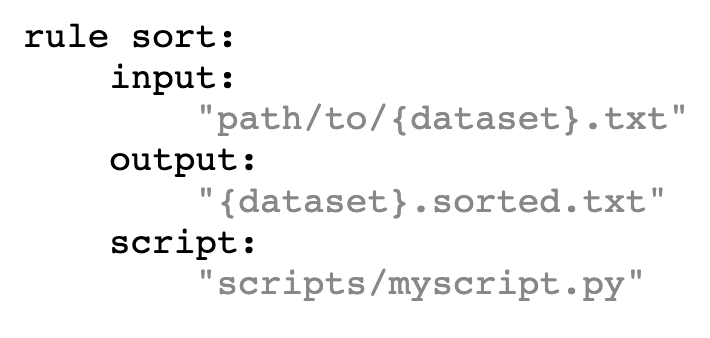
\includegraphics[width=\linewidth]{image/methods/rule}
      \end{figure}
      \source{Johannes K\"{o}ster (2019)}

  \end{columns}

  \note[item]{One of the most time consuming parts of phylogenetic analysis comes from the wrangling of datasets and fiddling with parameterizations}

\end{frame}

%------------------------------------------------

\begin{frame}

  \frametitle{Lassa workflow}
  \begin{figure}
    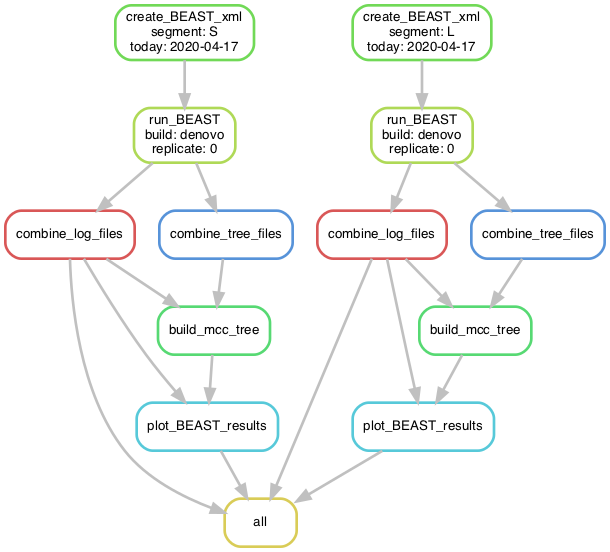
\includegraphics[width=.75\linewidth]{image/methods/workflow_dag}
  \end{figure}

  \note[item]{Work backwards through DAG}
  \note[item]{Only run rules if they are necessary (change in dataset or rule)}
  \note[item]{Individual rules can be run on HPC resources--computational efficiency (WIP)}
  \note[item]{Automatically support parallelization}

\end{frame}

%------------------------------------------------

\begin{frame}

  \frametitle{Online phylogenetic inference}

  \begin{itemize}
    \item We wish to leverage information from ongoing analyses when new data becomes available
    \item The state of an analysis is saved (checkpointed)
    \item New sequences are added via genetic distance-based sequence insertion
  \end{itemize}

  \begin{figure}
    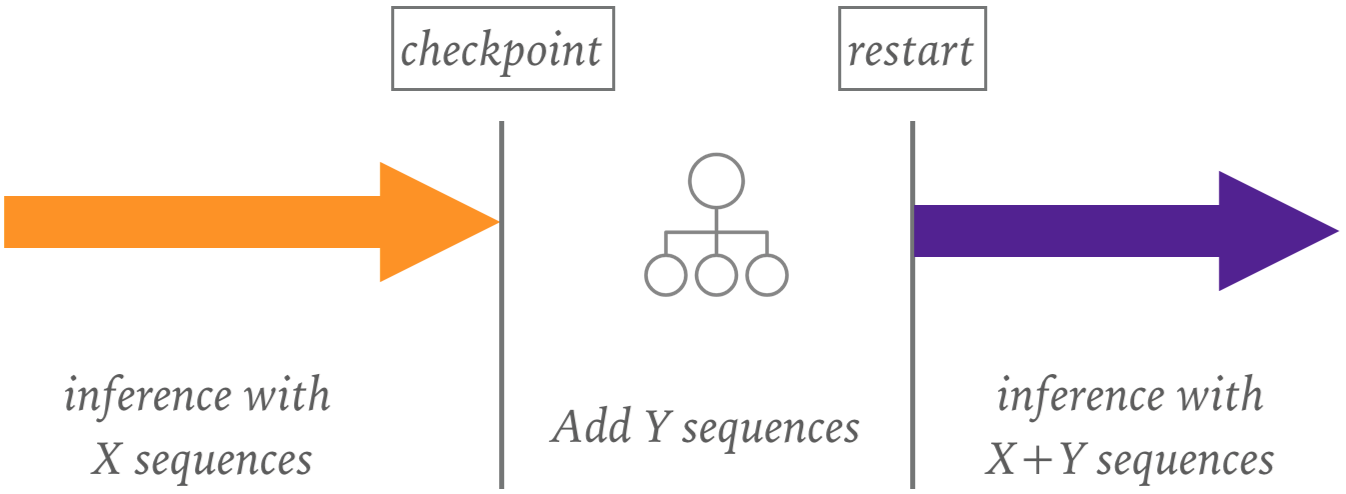
\includegraphics[width=.95\linewidth]{image/methods/online_beast}
  \end{figure}

  \note[item]{The current cutting edge of Bayesian phylogenetic analysis concerns ``online'' analyses}
  \note[item]{These analyses allow us to update the dataset we are analyzing by inserting new data, to leverage the results of existing analyses}
  \note[item]{This is very useful in the context of ongoing viral outbreaks in which we need to find actionable results quickly}

\end{frame}

%------------------------------------------------

\begin{frame}

  \frametitle{Evolutionary rate varies between segments}

  \begin{figure}
    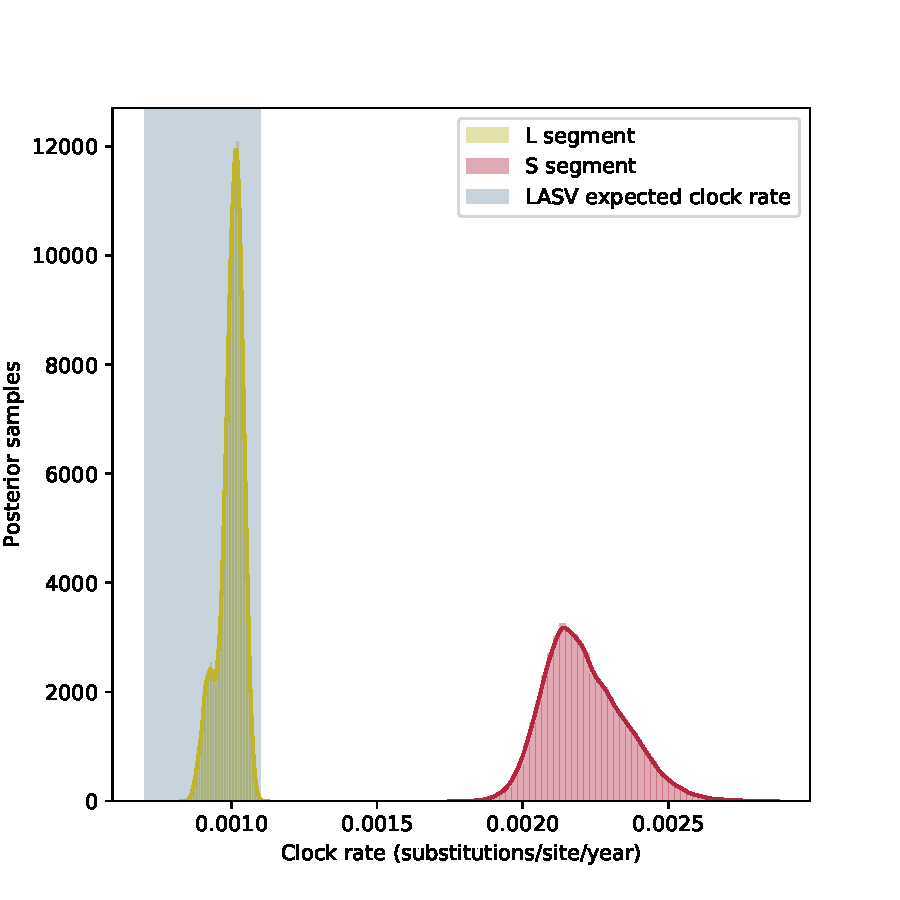
\includegraphics[width=.75\linewidth]{image/results/clock_rates_by_segment}
  \end{figure}

  \note[item]{Ran for 1.5 billion states over three replicates (2 months total compute time)}
  \note[item]{Chains still hadn't stabilized at that point}
  \note[item]{Our evo. rate estimates for L fit with the expectation from the literature}
  \note[item]{Our S estimate is 2x what is found in the literature}

\end{frame}

%------------------------------------------------

\begin{frame}

  \frametitle{Demographic history is conserved across segments}

  \begin{figure}
    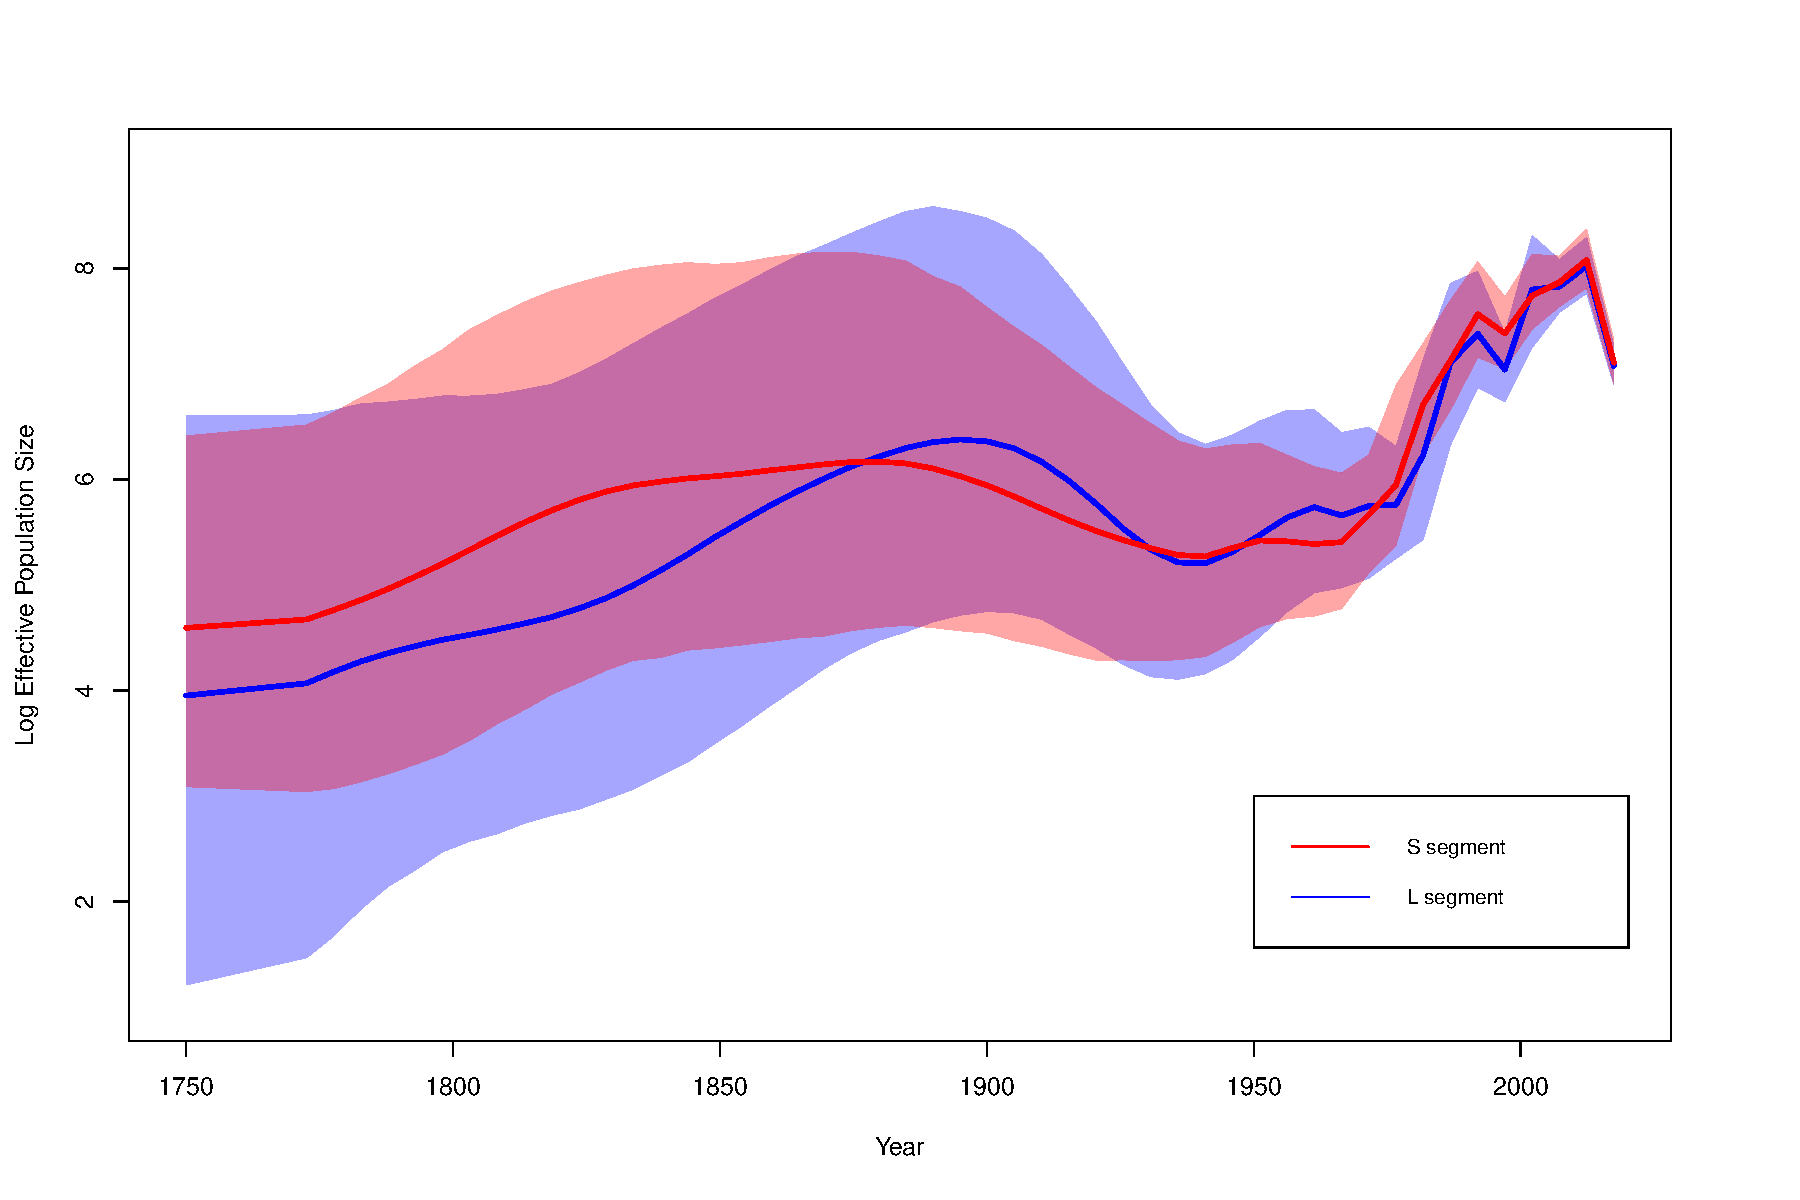
\includegraphics[width=\textwidth]{image/results/combined_skygrid}
  \end{figure}

  \note[item]{Despite differences in evo rates, we see similar demographic patterns between the segments, on similar time scales}
  \note[item]{Don't over describe the patterns, since HPD intervals are wide}

\end{frame}

%------------------------------------------------

\begin{frame}

  \frametitle{Future directions}

  \begin{enumerate}\itemsep=3ex
    \item Perform our analyses using more sophisticated, faster transition kernels
    \item Integrate existing Lassa pipeline with viral databasing tools (e.g. GLUE) to create seamless workflows
    \item Extend online BEAST to accommodate more complex phylogenetic models
  \end{enumerate}

  \note[item]{We will use the HMC operator for branch rates, rather than just demographic modeling}
  \note[item]{Consider briefly explaining how HMC differs from block operator}
  \note[item]{The pipeline that has been presented should interplay nicely with sequence databases, allowing for new online builds to be triggered when new data becomes available}
  \note[item]{Current online BEAST implementation hasn't been fully worked out for complex models}
  \note[item]{Model switching partway through an outbreak is desirable}

\end{frame}

%------------------------------------------------
\section{Conclusion}
%------------------------------------------------

\begin{frame}
  \frametitle{Acknowledgments}
  \begin{columns}[c] % The "c" option specifies centered vertical alignment while the "t" option is used for top vertical alignment

    \column{.4\textwidth} % Left column and width

    Guy Baele

    Mandev Gill

    \vspace{5mm}

    Marijn Thijssen

    N\'{i}dia Sequeira Trov\~{a}o

    Mahmoud Reza~Pourkarim

    \vspace{5mm}

    Liana Kafetzopoulou

    Simon Dellicour

    \column{.27\textwidth} % Right column and width

    Samuel Hong

    Kanika Nahata

    Ine Boonen

    Yiqiao Li

    Jade Membrebe

    Nena Bollen

    Magda Bletsa

    \vspace{5mm}

    Gytis Dudas

    \column{.33\textwidth} % Right column and width

    KU Leuven

    Rega Institute

    \vspace{5mm}

    Belgian American Education Foundation

    \vspace{5mm}

    
\includegraphics[width=.75\linewidth]{image/baef_logo}

  \end{columns}
\end{frame}

%----------------------------------------------------------------------------------------

\appendix

% %------------------------------------------------
%
\begin{frame}
  \Huge{\centerline{Additional slides}}
\end{frame}

%------------------------------------------------

\begin{frame}
  \frametitle{HBV-A subgenotyping}
  \begin{figure}
    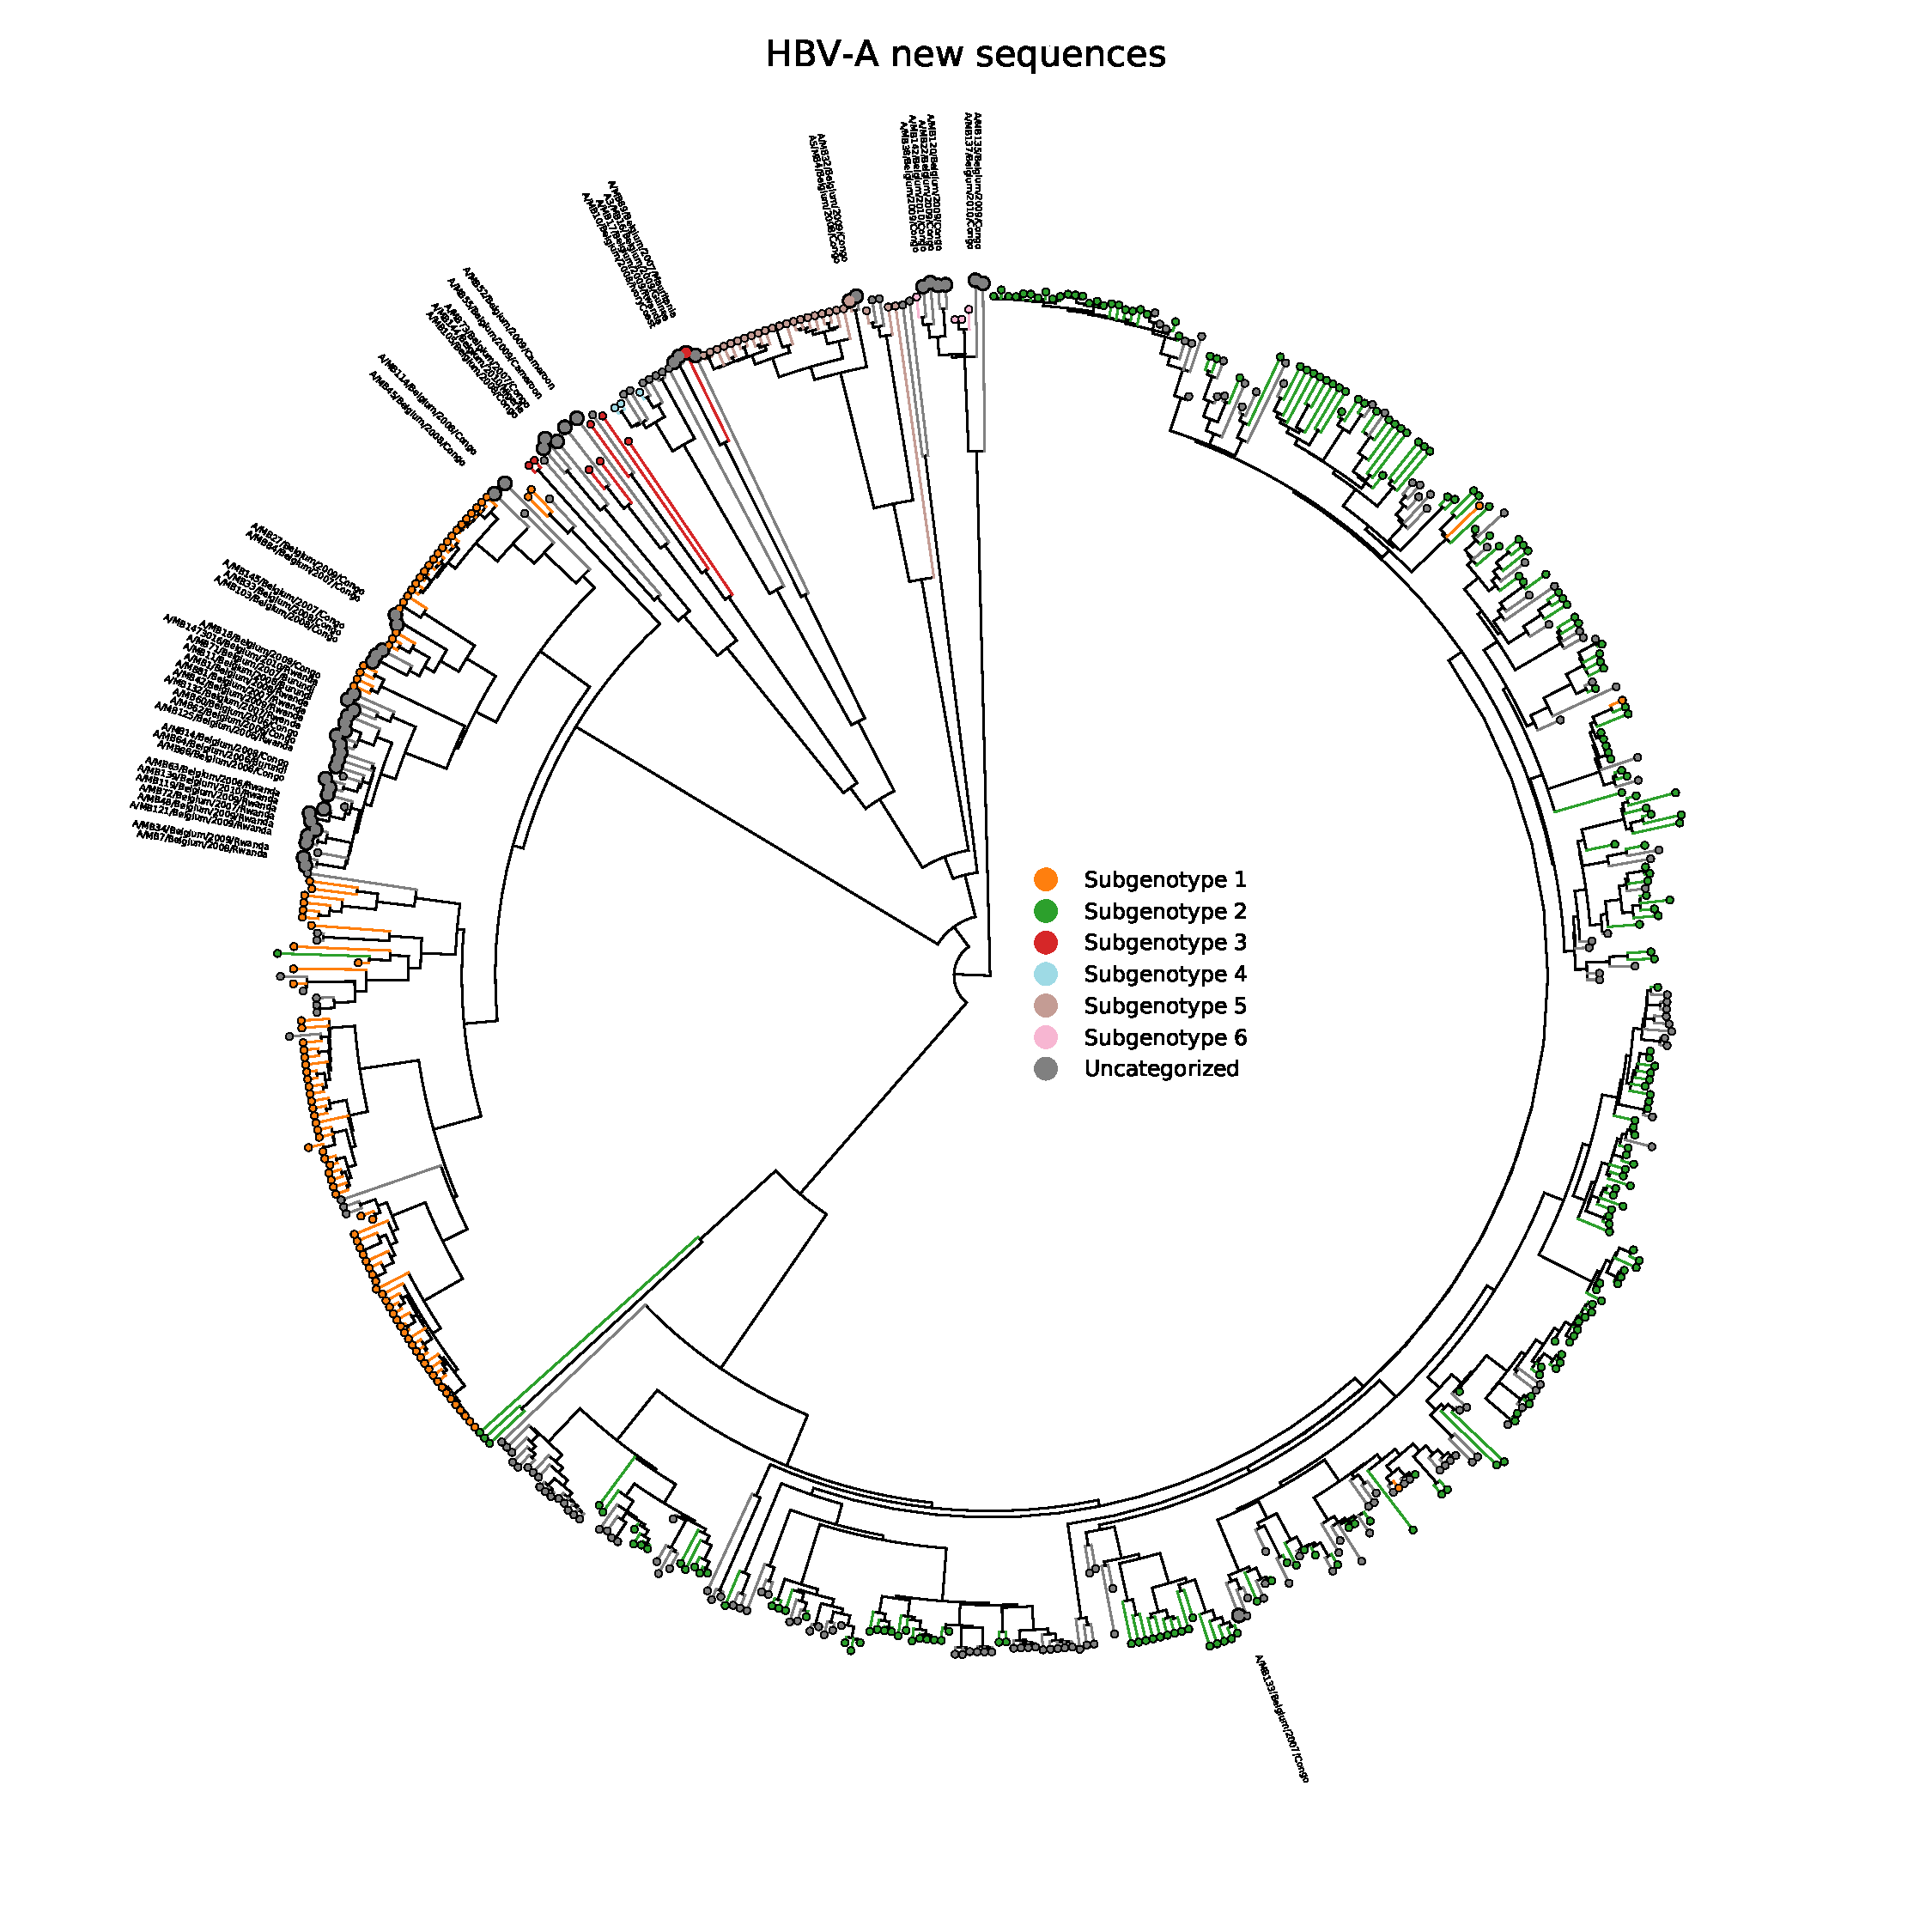
\includegraphics[width=.6\linewidth]{image/results/HBV-A_new_sequences}
  \end{figure}
\end{frame}

%------------------------------------------------

\begin{frame}
  \frametitle{HBV-A subgenotyping}
  \begin{figure}
    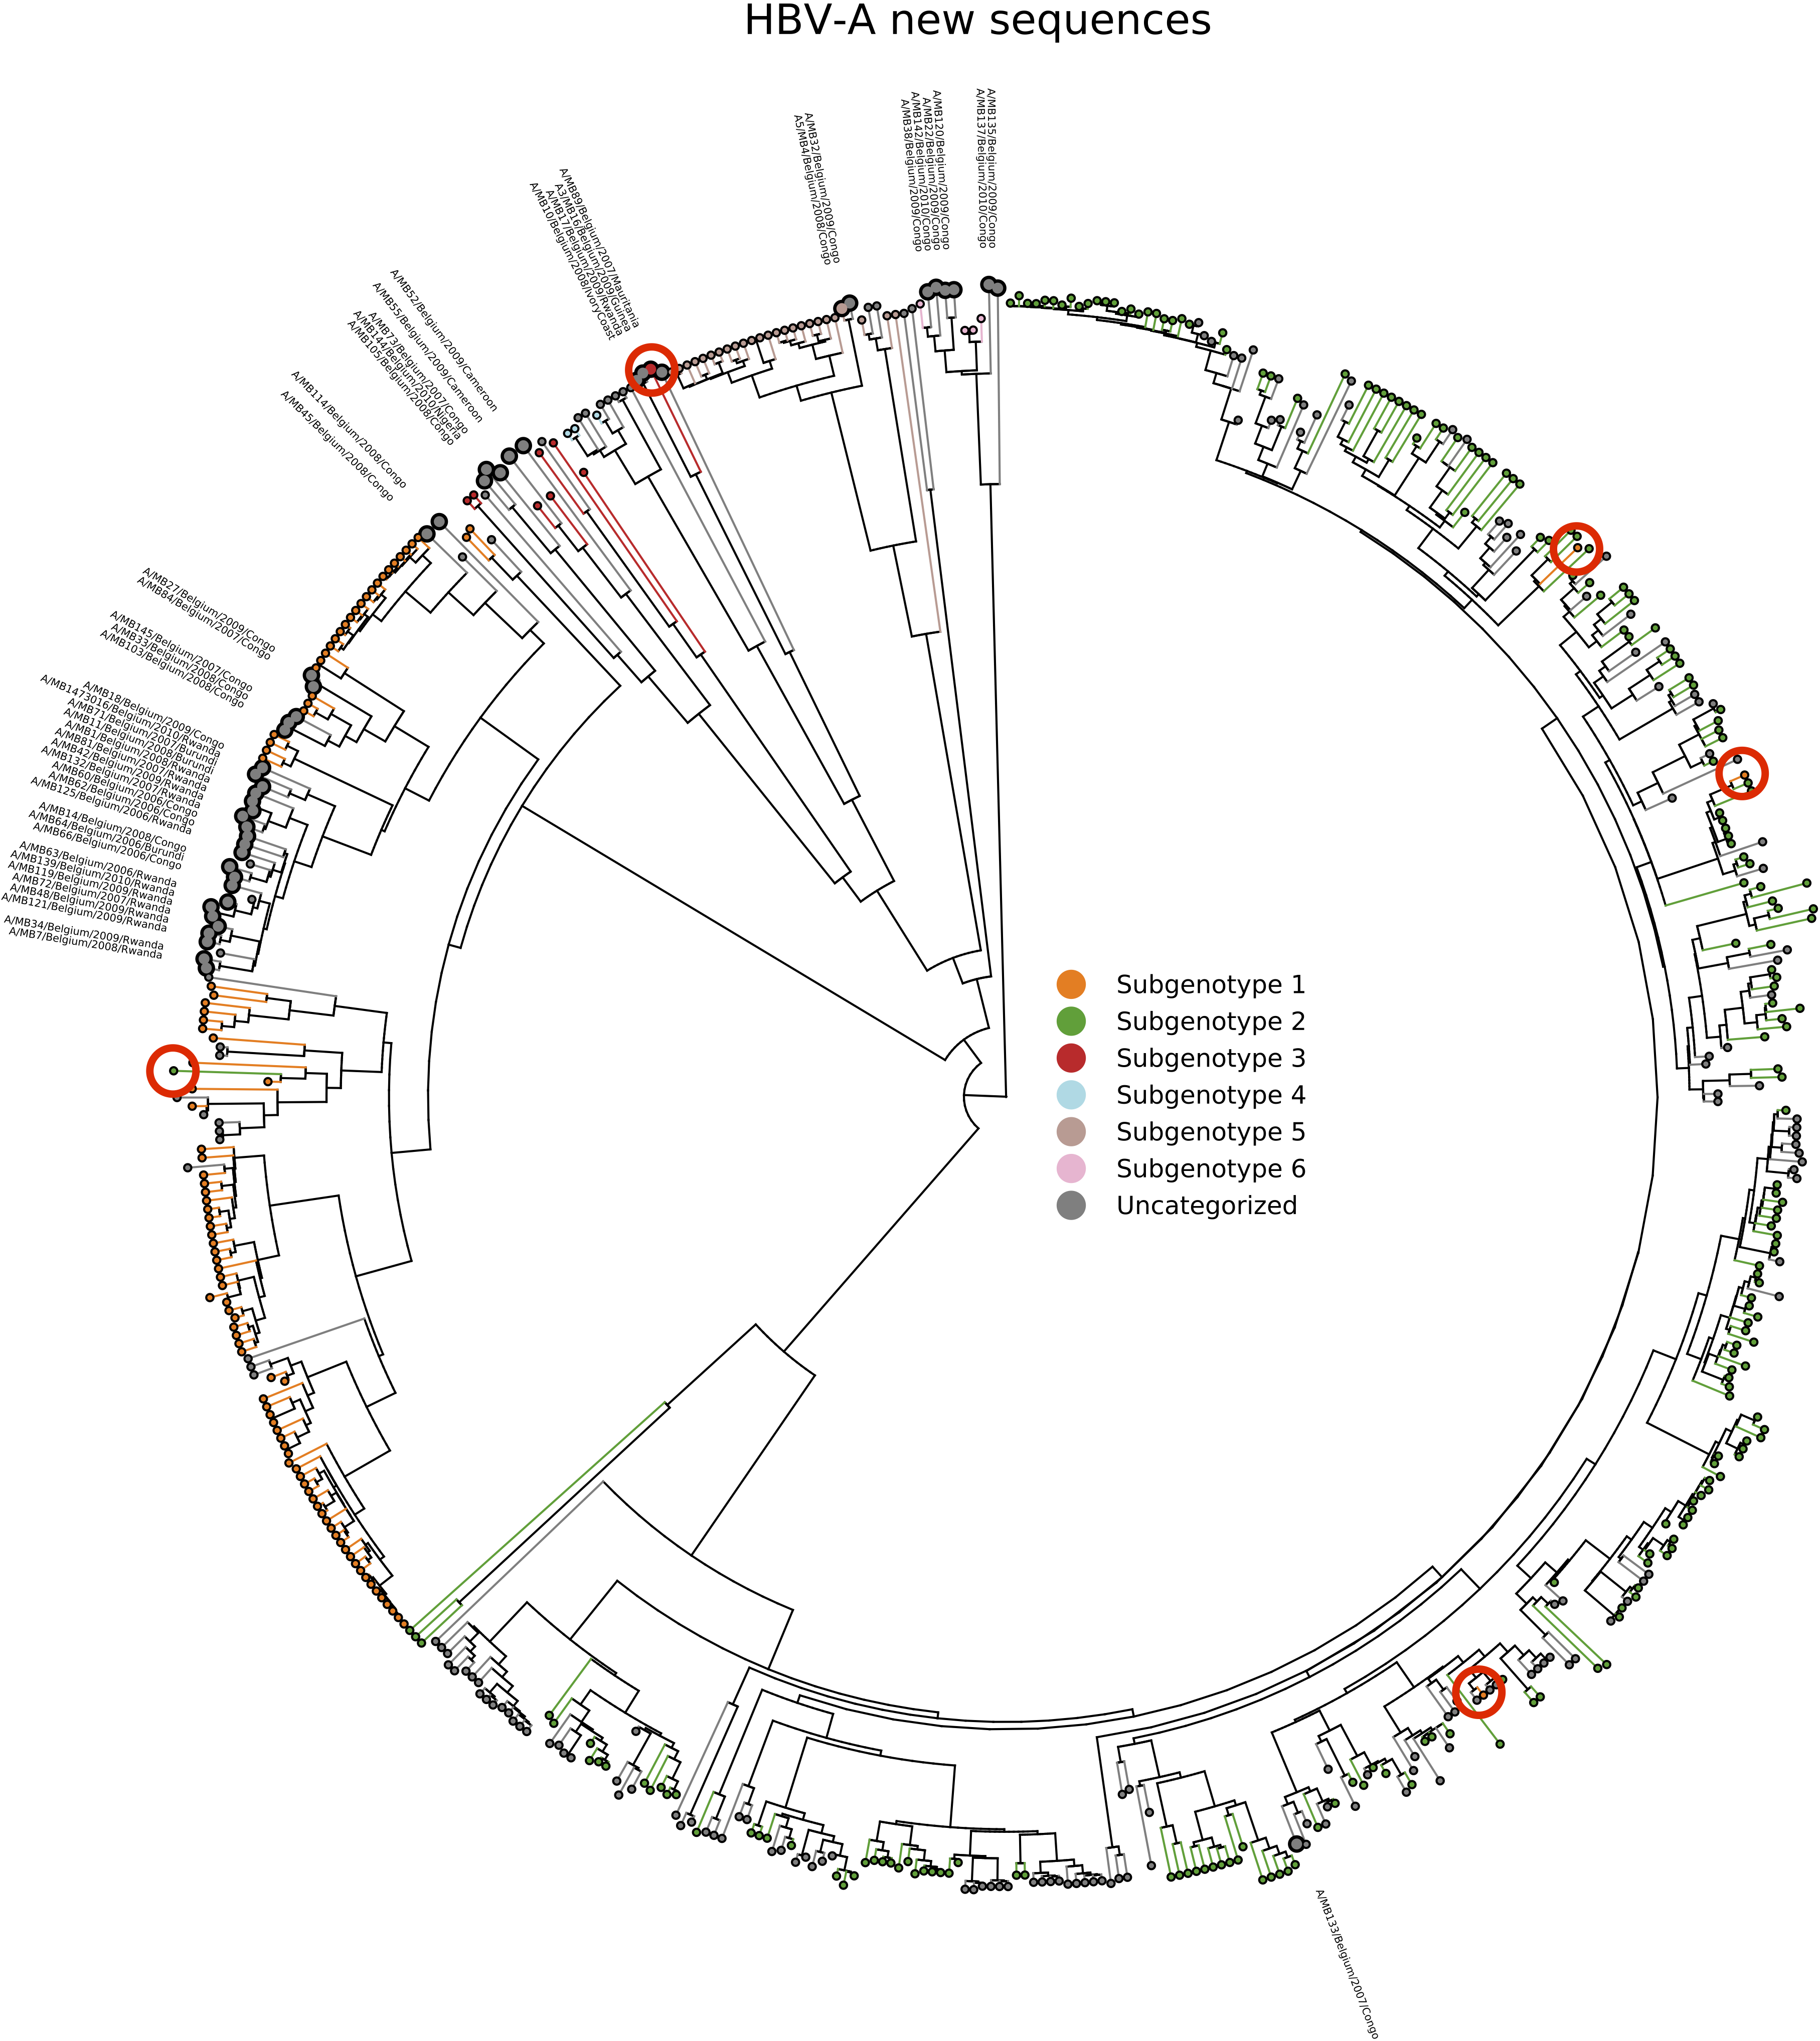
\includegraphics[width=.6\linewidth]{image/results/HBV-A_new_sequences_with_highlights.png}
  \end{figure}
\end{frame}

%------------------------------------------------

\begin{frame}
  \frametitle{HBV-D subgenotyping}
  \begin{figure}
    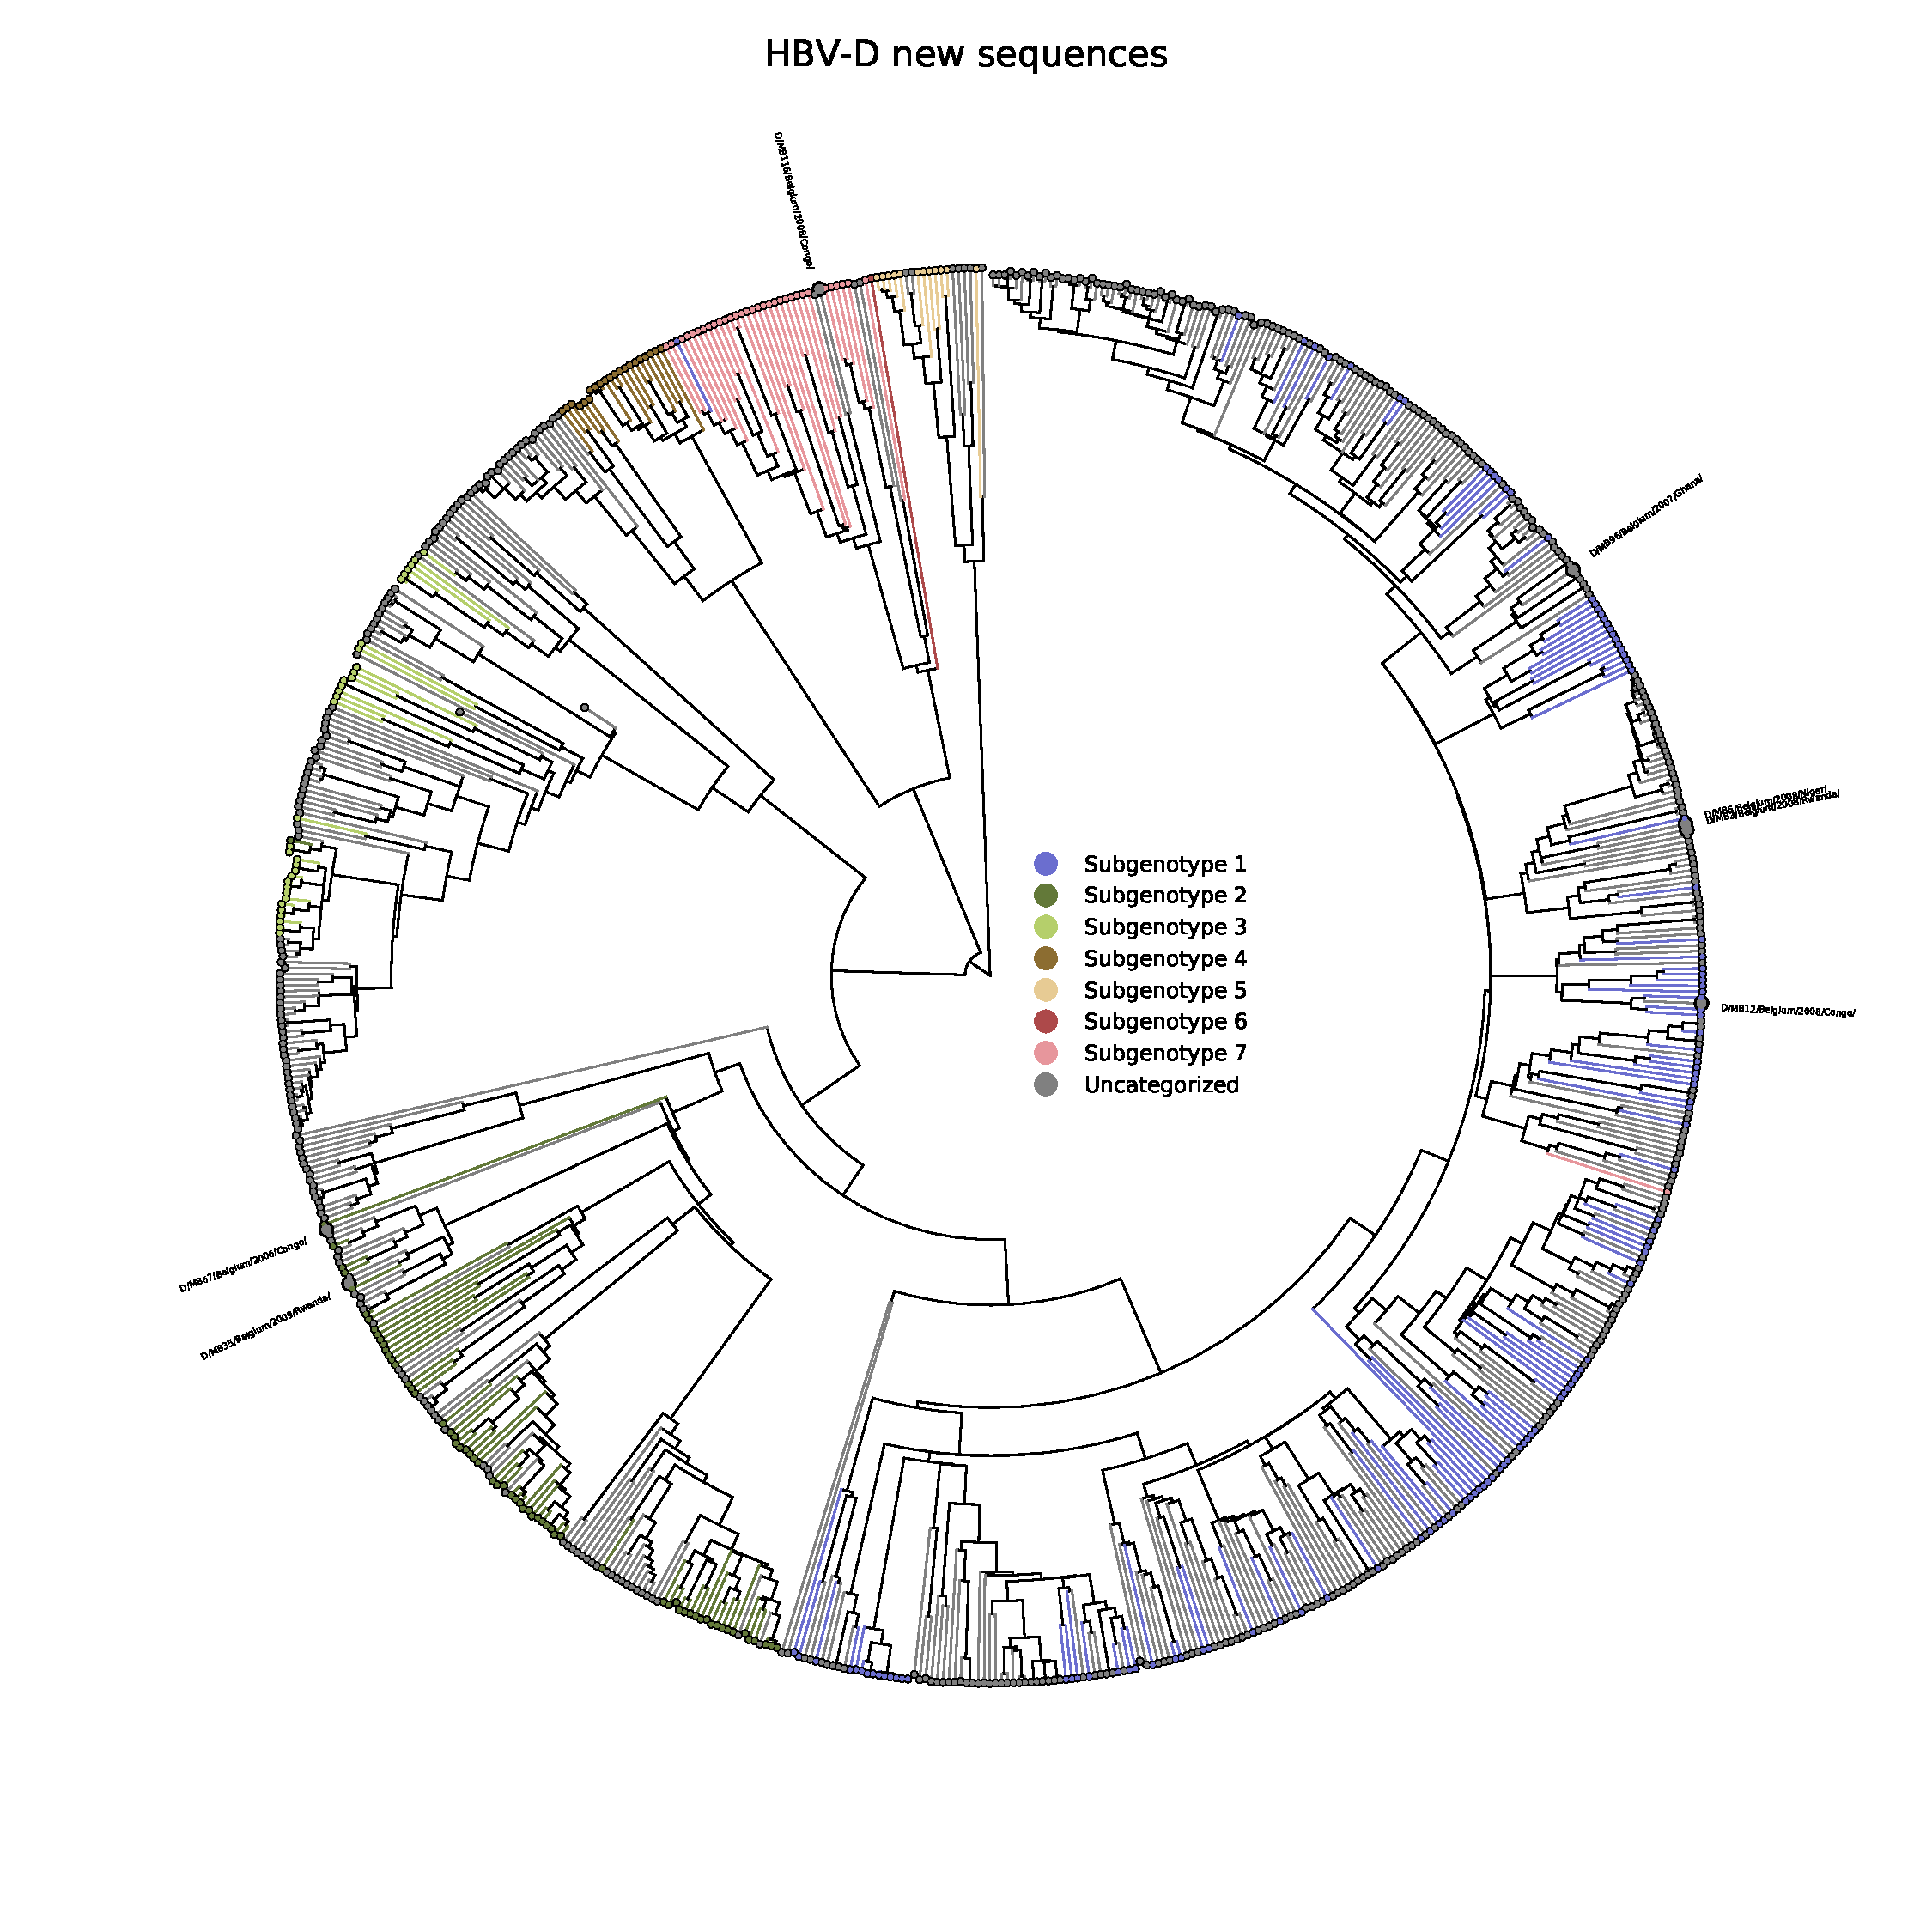
\includegraphics[width=.6\linewidth]{image/results/HBV-D_new_sequences}
  \end{figure}
\end{frame}

%------------------------------------------------

\begin{frame}
  \frametitle{HBV-D subgenotyping}
  \begin{figure}
    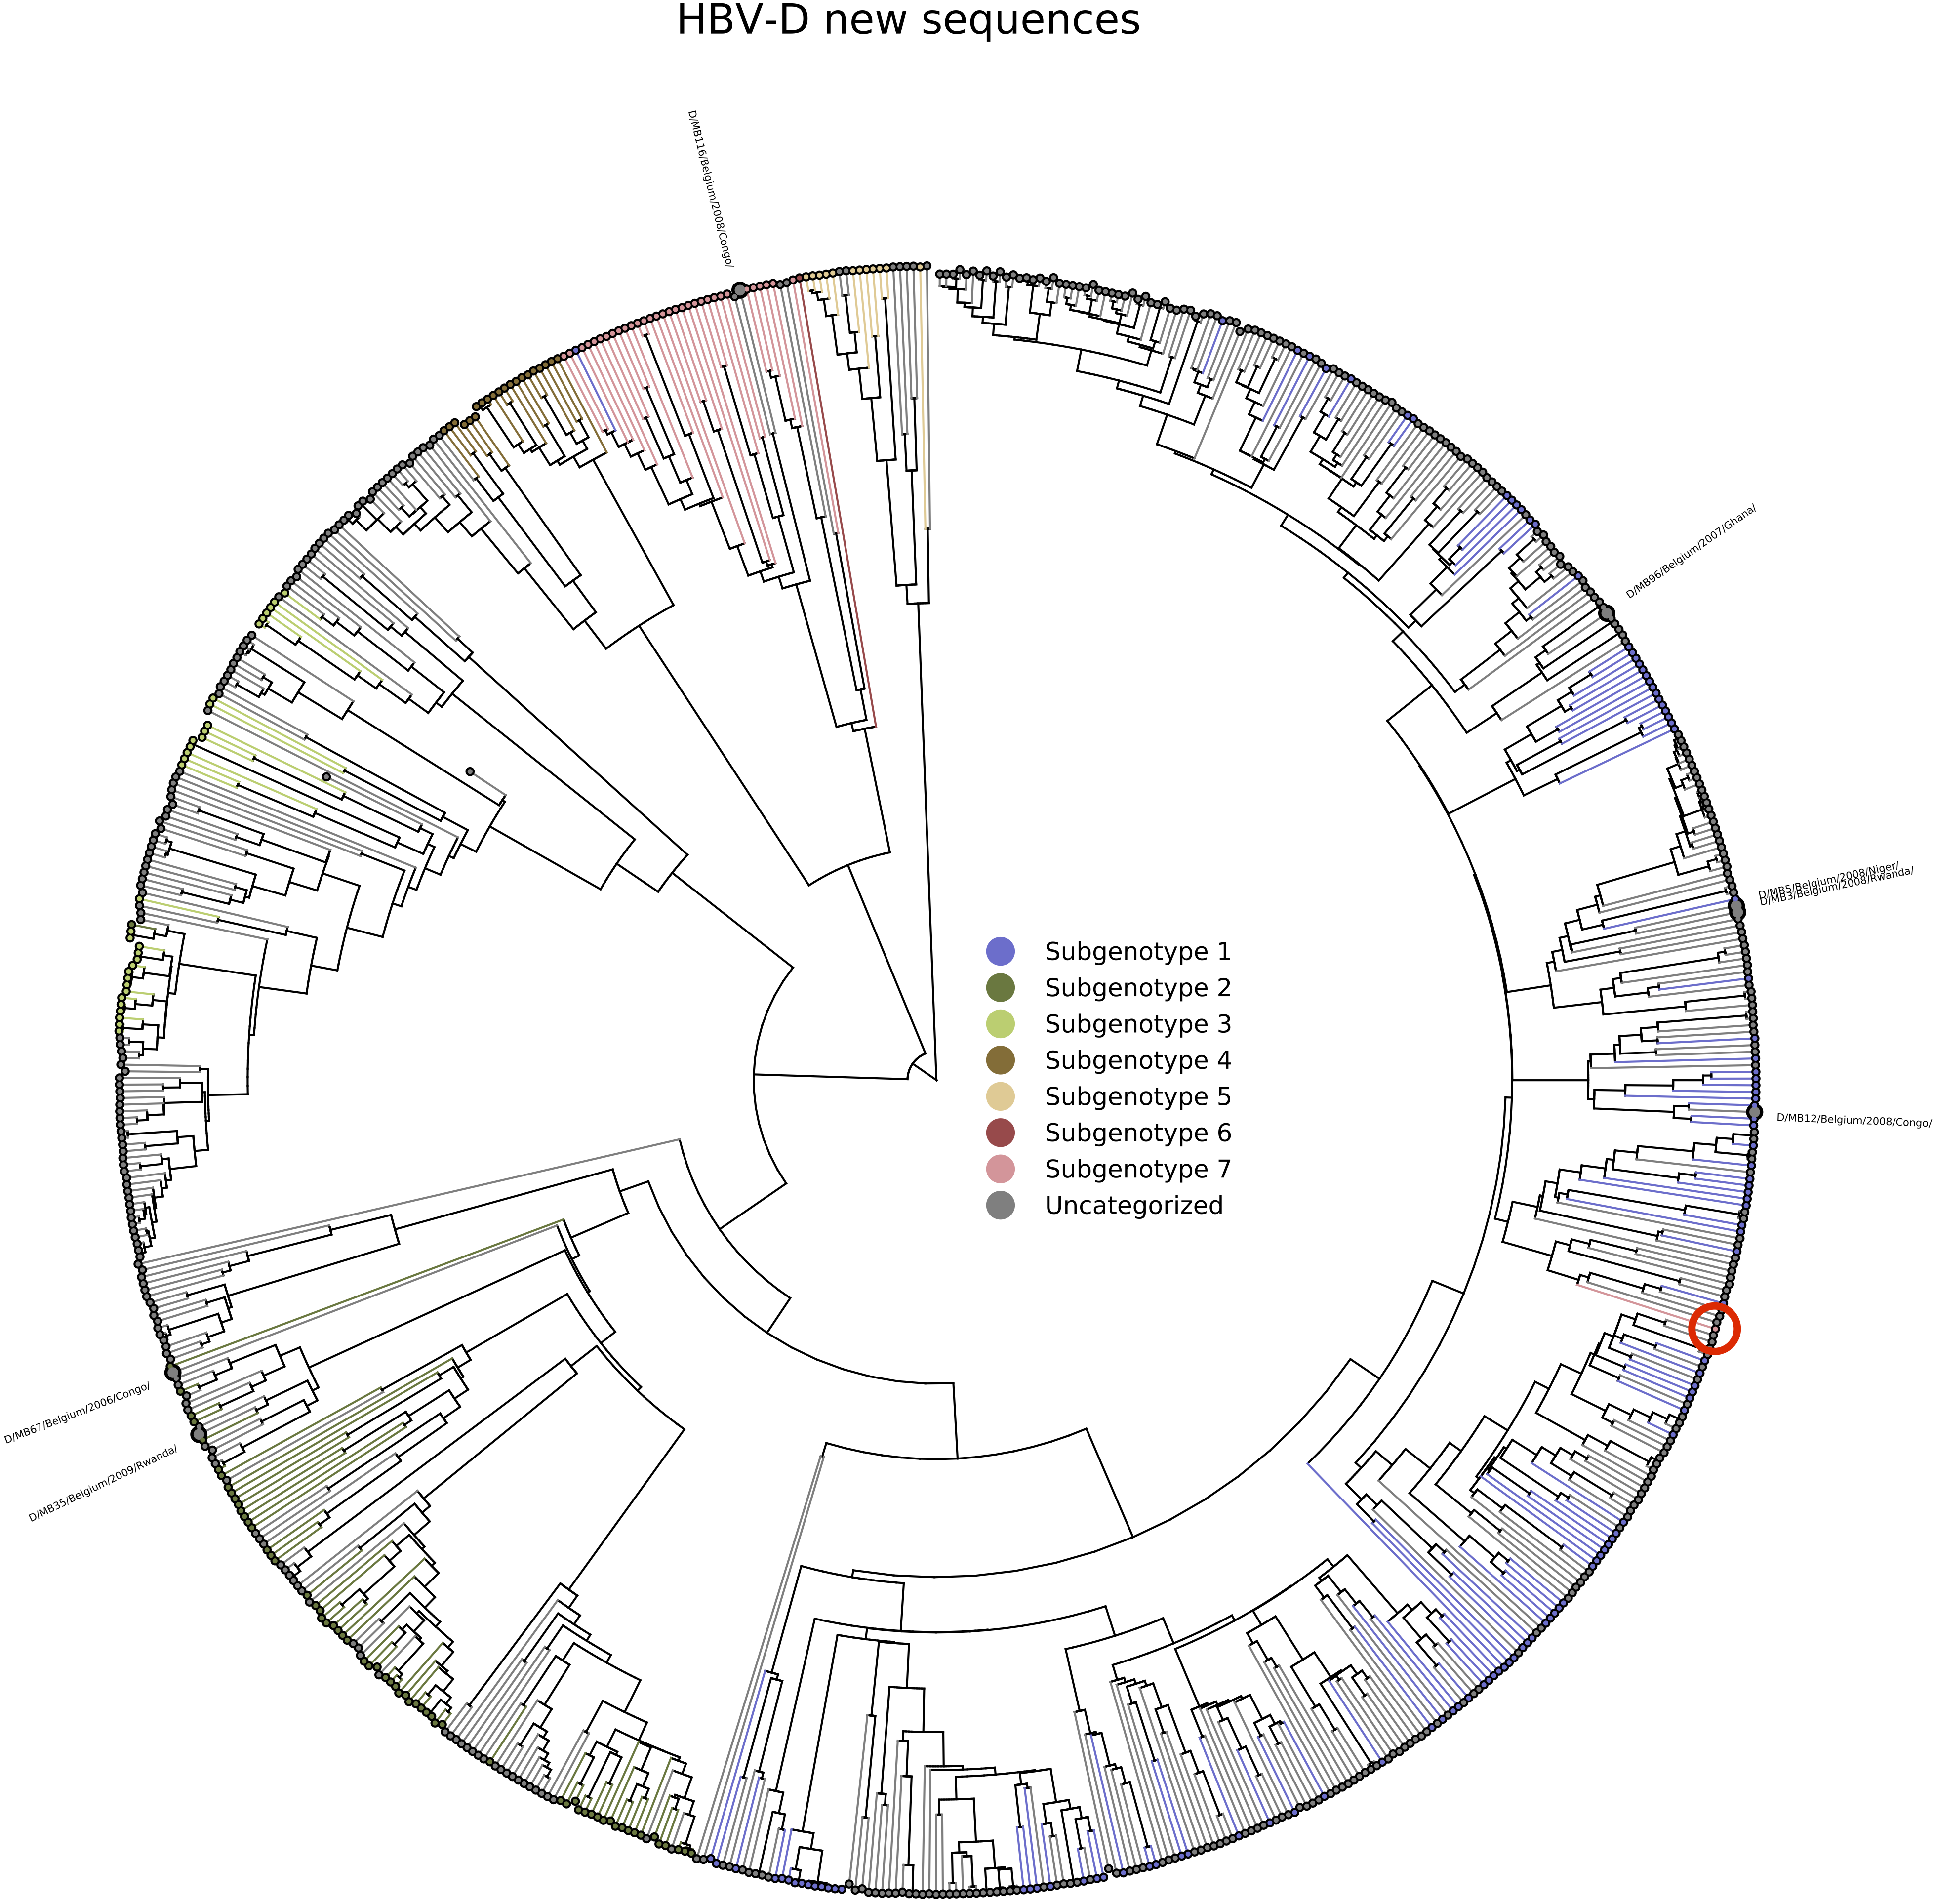
\includegraphics[width=.6\linewidth]{image/results/HBV-D_new_sequences_with_highlights.png}
  \end{figure}
\end{frame}

%------------------------------------------------

\begin{frame}

  \frametitle{Bayesian phylogenetic inference}

  \begin{columns}[c]

    \column{0.5\textwidth}

      \begin{equation*}
      \begin{aligned}
        P(T, \boldsymbol\mu,{} &\boldsymbol f, \theta) \\
        & \propto P(S \vert T, t_{I}, \boldsymbol\mu) \\
        & \times P(L \vert T, t_{I}, \boldsymbol f) \\
        & \times P(T \vert t_{I}, \theta) \\
        & \times P(\boldsymbol\mu,\boldsymbol f,\theta)
      \end{aligned}
    \end{equation*}

    \column{.5\textwidth}
      \begin{figure}
        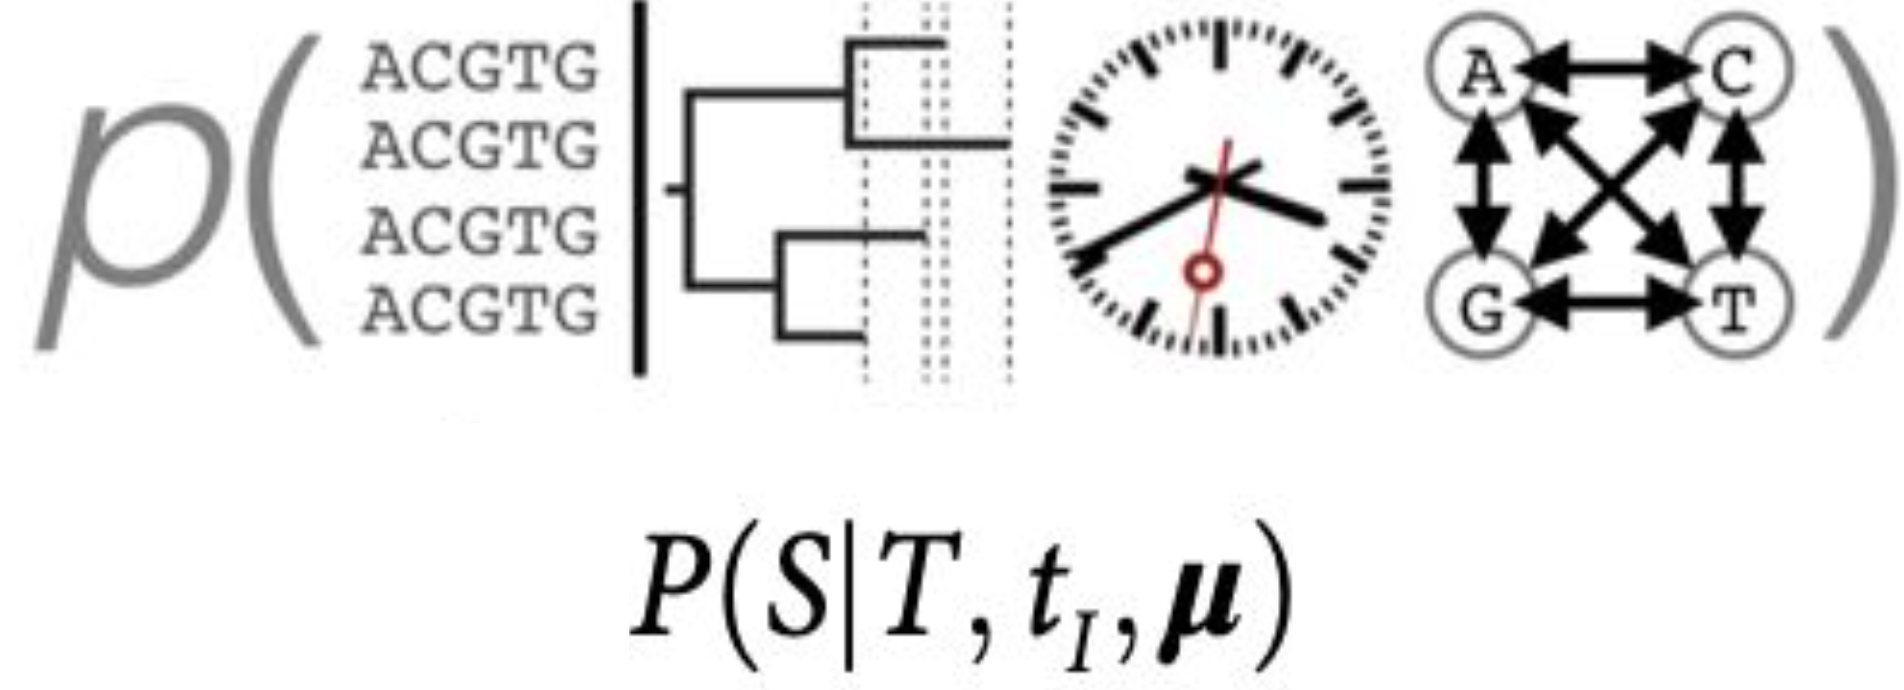
\includegraphics[height=4em]{image/intro/p_alignment}
      % \end{figure}
      % \begin{figure}

        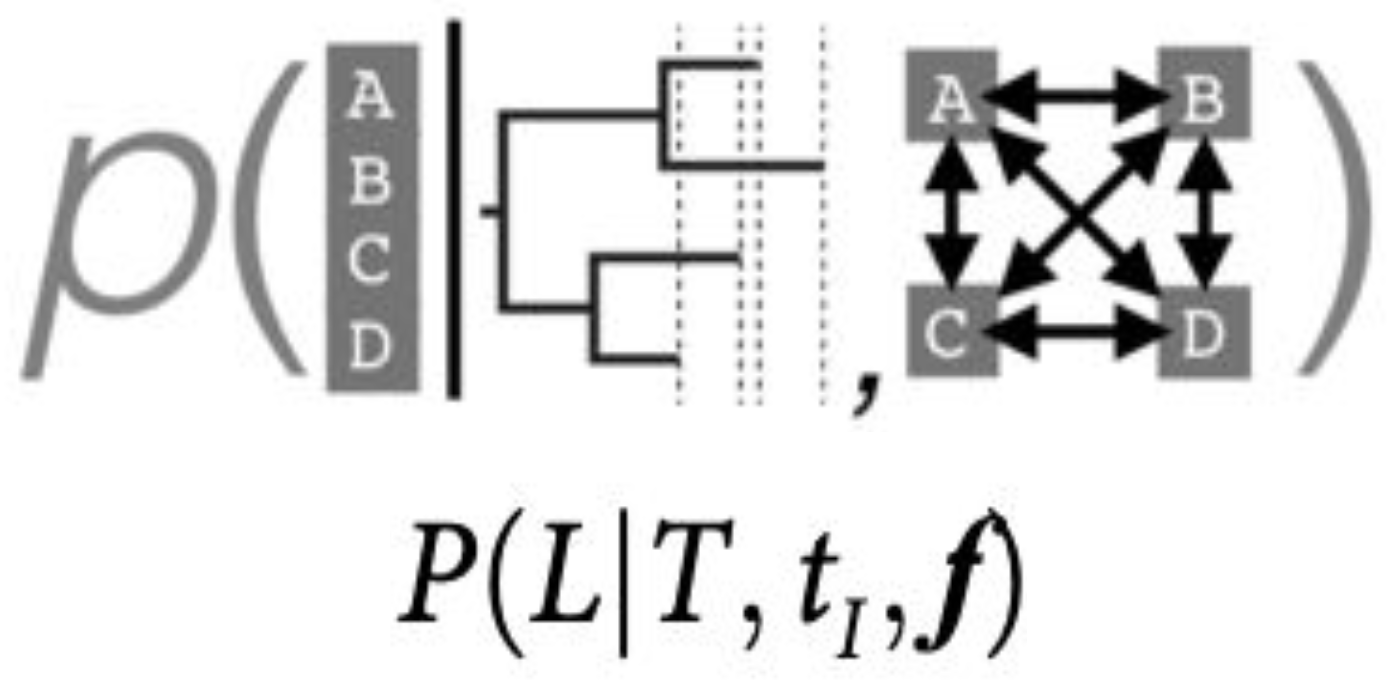
\includegraphics[height=4em]{image/intro/p_locations}
      % \end{figure}
      % \begin{figure}

        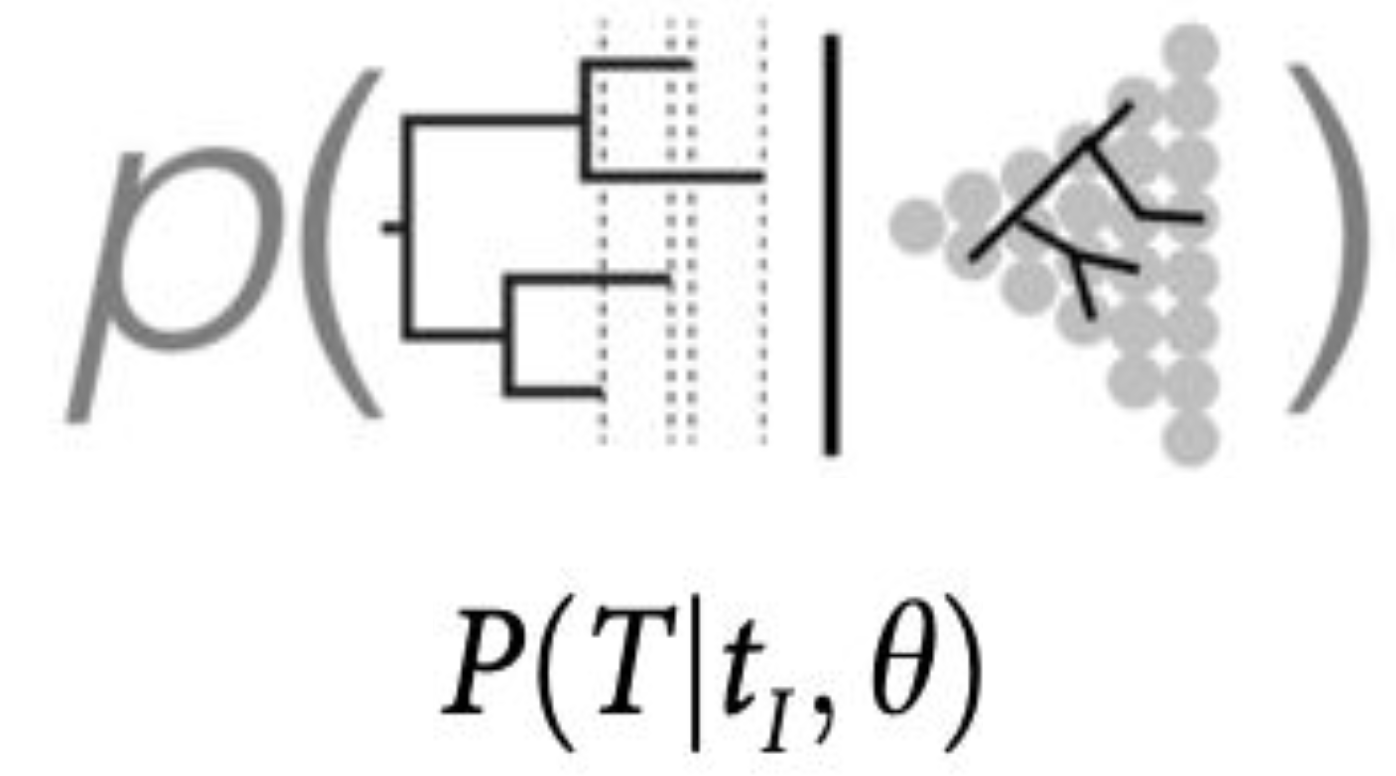
\includegraphics[height=4em]{image/intro/p_demographics}
      \end{figure}

  \end{columns}

  \note[item]{We perform our analysis under a Bayesian framework.}
  \note[item]{Posterior probability of our inferred parameters is proportional to the joint conditional probabilities:}
  \note[item]{Alignment given tree, sampling times, and mutation rates}
  \note[item]{Observed locations given tree, sampling times, and migration rates}
  \note[item]{Tree given sampling times and demographic history}
  \note[item]{We also have priors for the parameters that we infer.}

\end{frame}

%------------------------------------------------

\begin{frame}

  \frametitle{We traverse state space using MCMC}

  \begin{figure}
    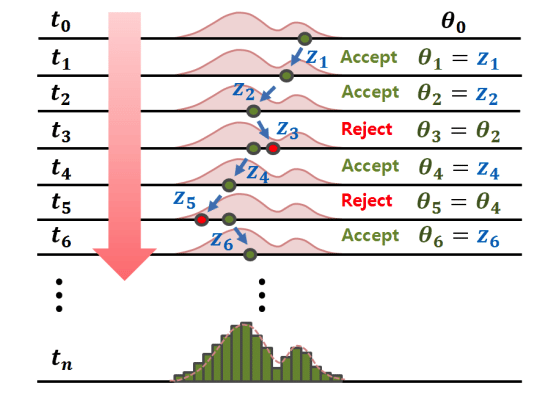
\includegraphics[width=.8\textwidth]{image/intro/mcmc_illustration}
    \source{Jin, Ju, \& Jung (2019)}
  \end{figure}

  \note[item]{We can use the same type of algorithm to explore the state space of other parameters we are interested in (evolutionary rates, migration rates, population sizes)}
  \note[item]{Highlight that as we log the state of the chain over time we recover a distribution for each parameter, not a point estimate}

\end{frame}

%------------------------------------------------

\begin{frame}

  \frametitle{A note on temporal signal}

  \begin{figure}
    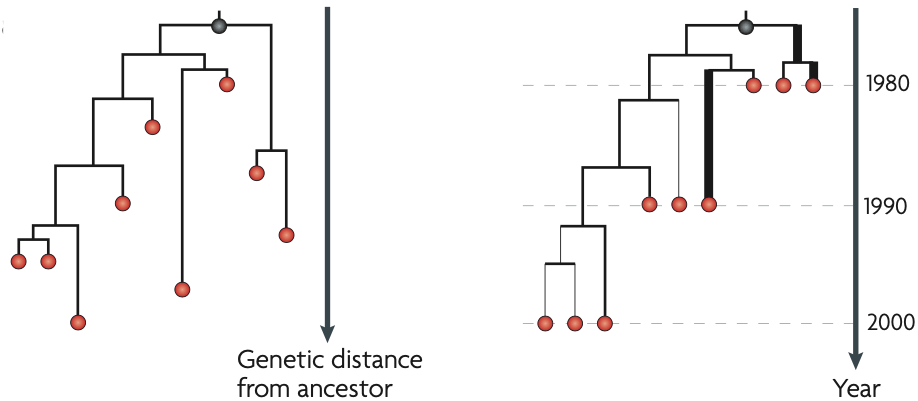
\includegraphics[width=.95\linewidth]{image/intro/temporal_signal}
  \end{figure}
  \source{Pybus \& Rambaut (2009)}

\end{frame}

%------------------------------------------------

\begin{frame}

  \frametitle{Clock-like evolutionary rates are desirable}

  \begin{figure}
    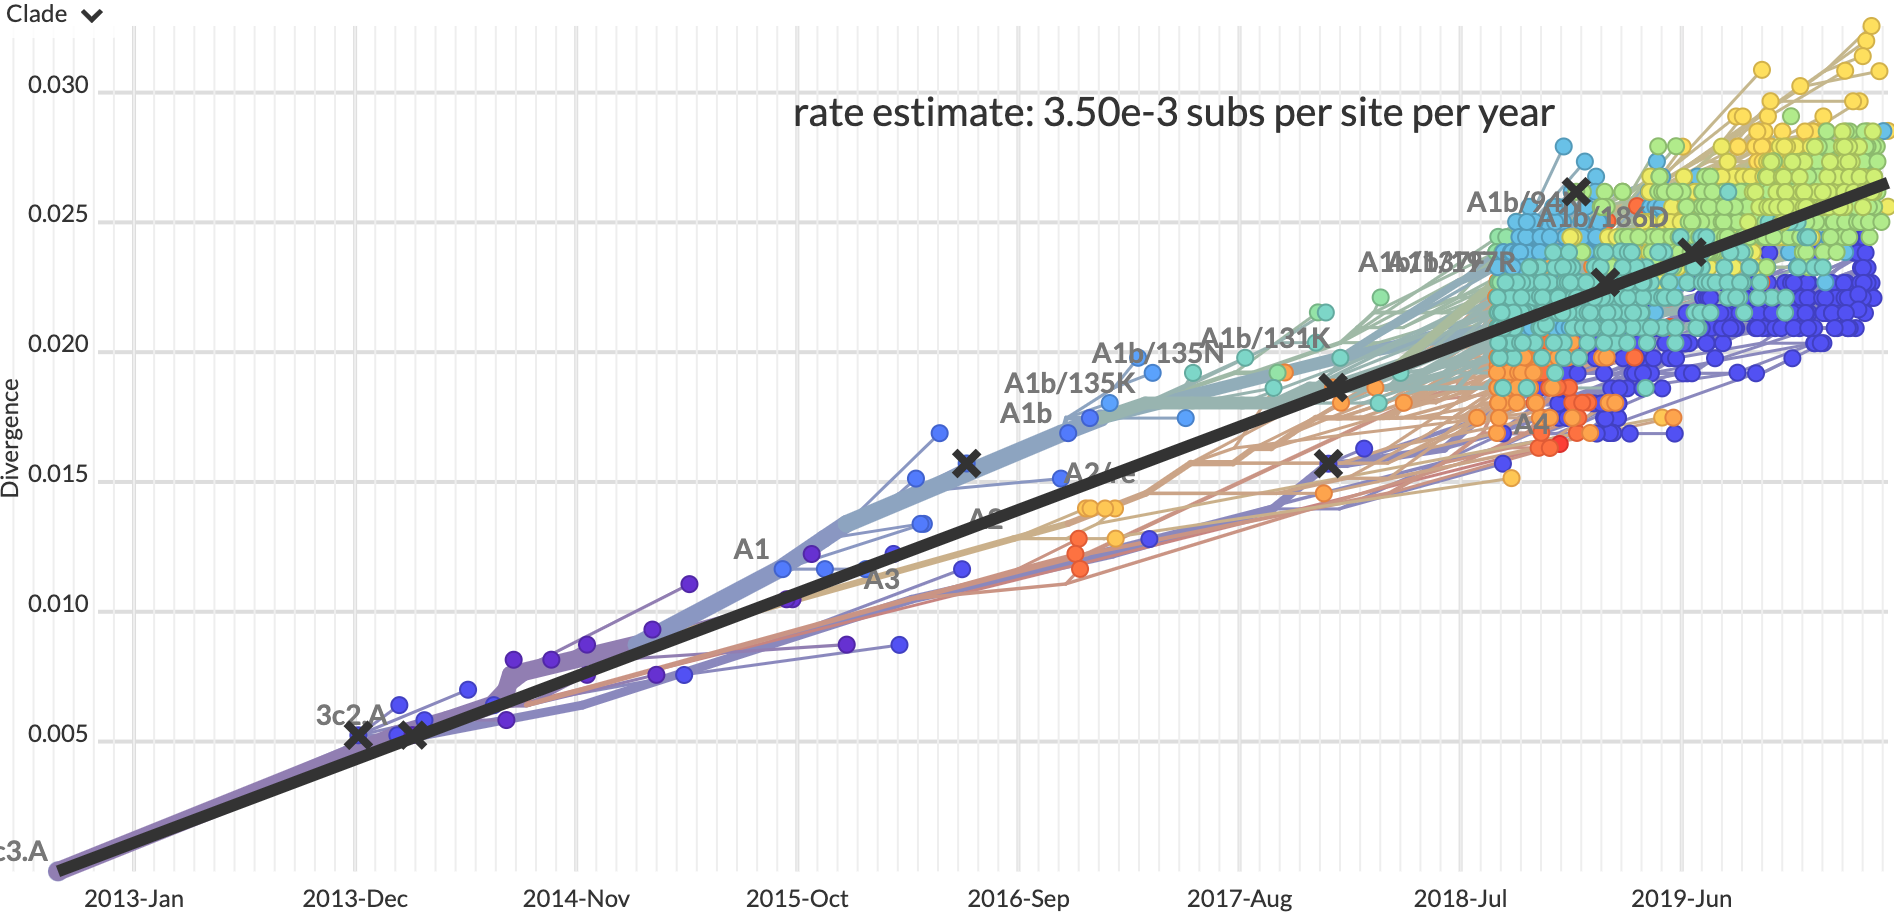
\includegraphics[width=.95\linewidth]{image/intro/nextstrain_flu_clock}
  \end{figure}
  \source{nextstrain.org}

  \note[item]{We can determine whether there is sufficient ``temporal signal'' in a dataset by constructing a root-to-tip divergence over time plot and determining if a linear regression fits the data.}

\end{frame}

%------------------------------------------------

\begin{frame}

  \frametitle{Online BEAST facilitates analysis in real-time}

  \begin{figure}
    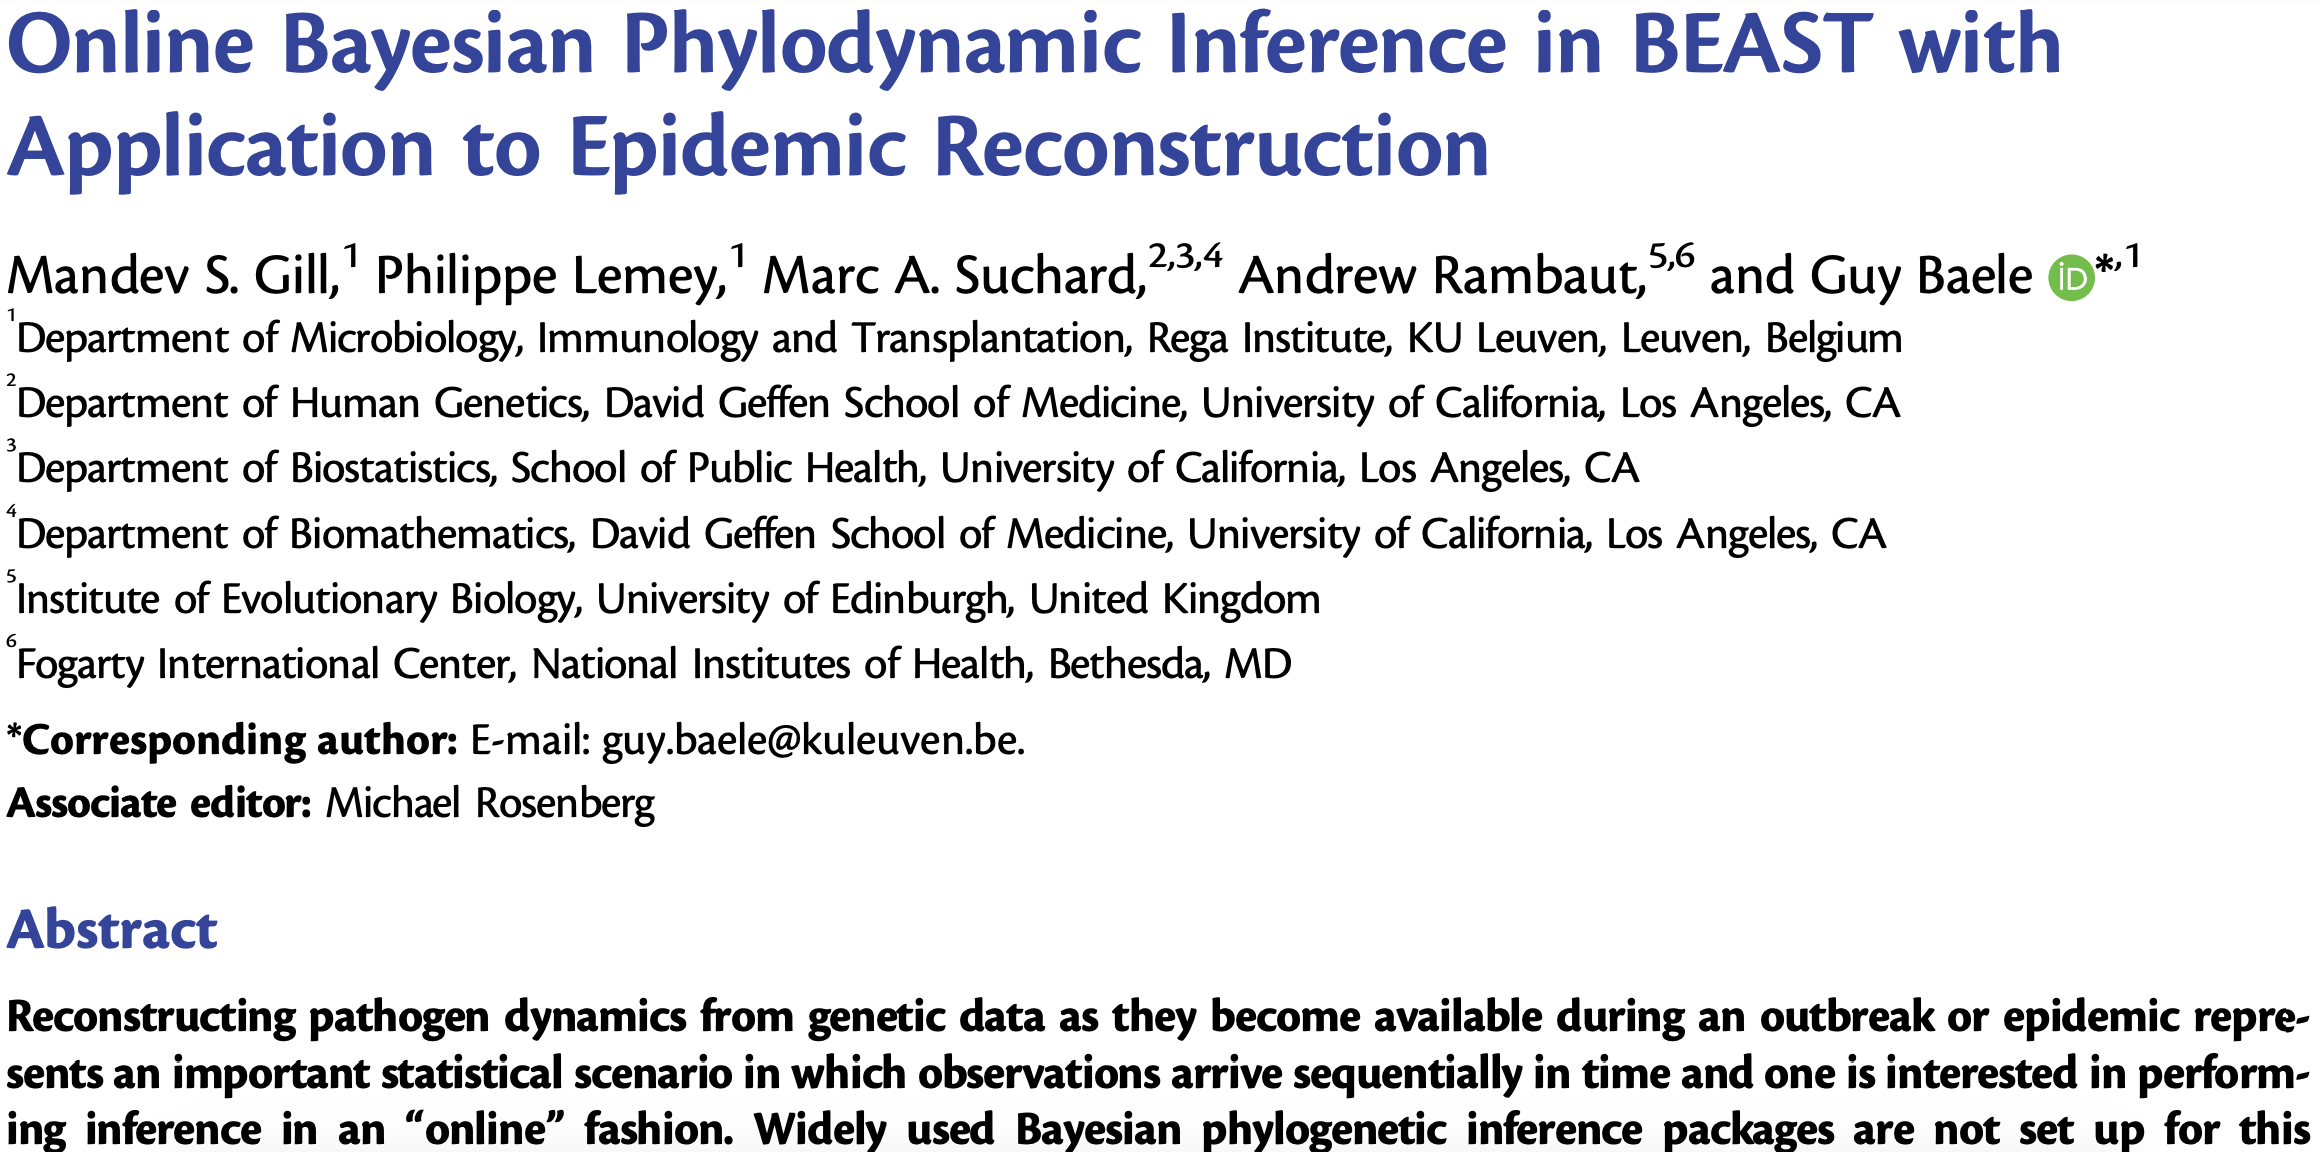
\includegraphics[width=.85\linewidth]{image/intro/online_beast_paper}
  \end{figure}

\end{frame}

%------------------------------------------------

\begin{frame}

  \frametitle{Online BEAST facilitates analysis in real-time}

  \begin{figure}
    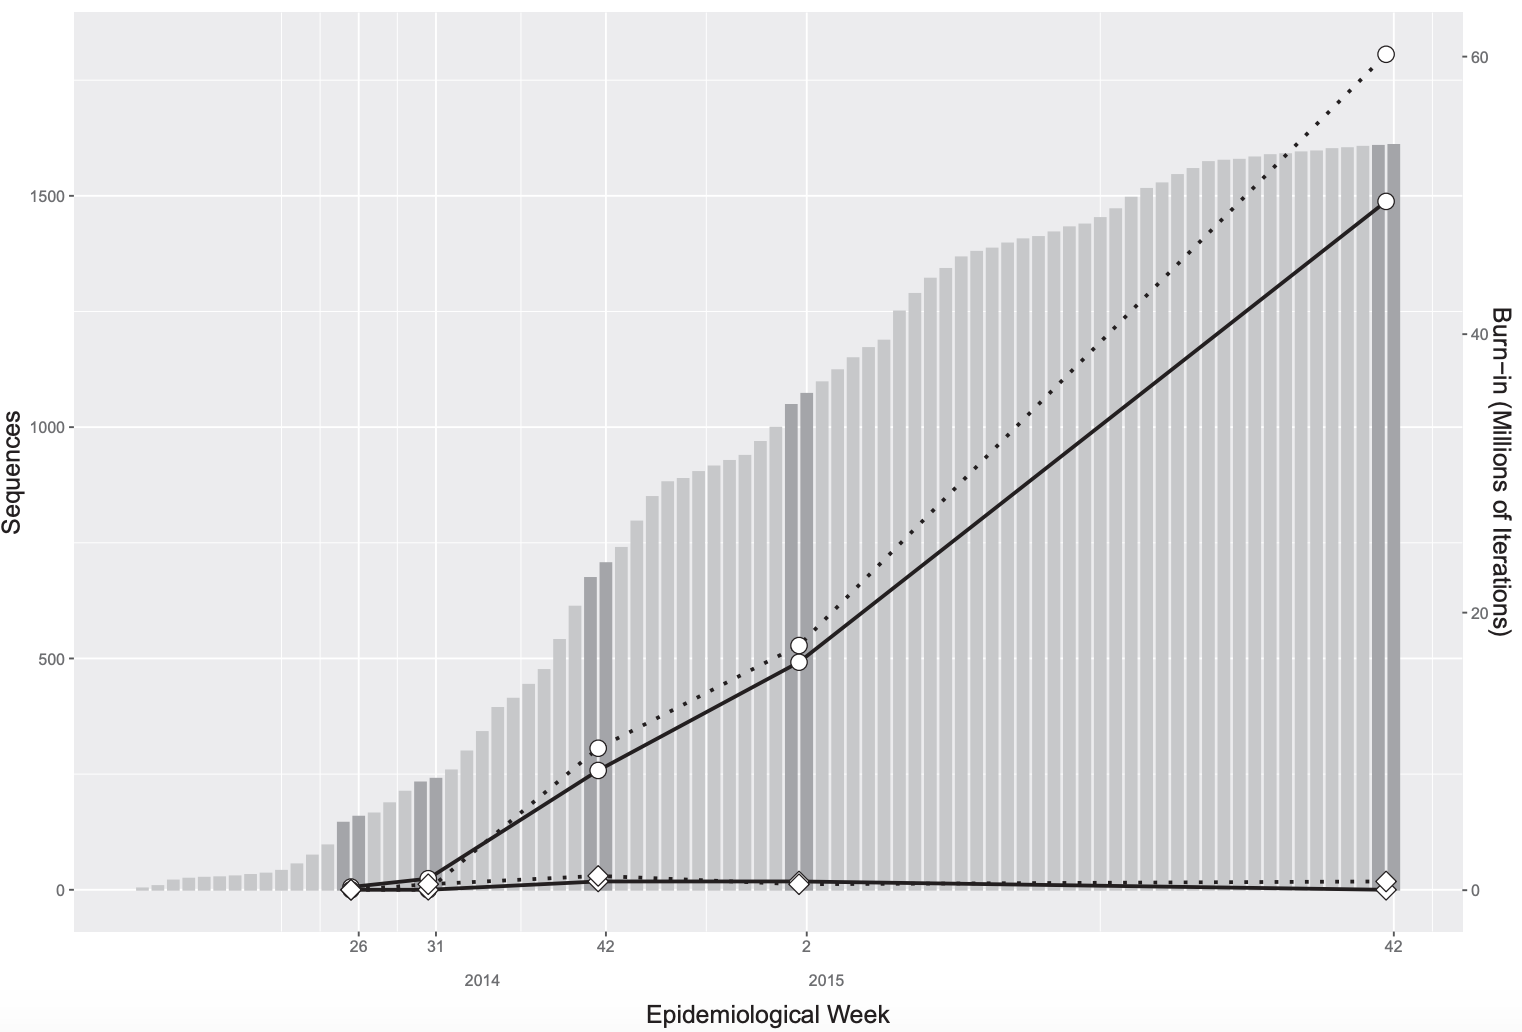
\includegraphics[width=.95\linewidth]{image/intro/online_beast}
  \end{figure}

  \note[item]{De novo analyses can take a very long time to ``burn in''; online analysis reduces that burden}
  \note[item]{Summarize figure}
  \note[item]{Online analyses frequently require exact duplication of pipelines, and are aided by easy addition of new data (i.e. data acquisition and alignment)}
  \note[item]{The pipeline that I describe here makes this process much smoother}
  \note[item]{Briefly talk about how it was used for SARS-CoV-2 during the early parts of the pandemic}

\end{frame}

%------------------------------------------------

\end{document}

% \begin{frame}
%   \frametitle{References}
%   \footnotesize{
%     \begin{thebibliography}{99} % Beamer does not support BibTeX so references must be inserted manually as below
%
%       \bibitem[Paules, 2017]{paules2017what} Catharine I. Paules, MD; Robert W. Eisinger, PhD; Hilary D. Marston, MD, MPH; and Anthony S. Fauci, MD (2017)
%       \newblock What recent hisotory has taught us about responding to emerging infectious disease threats
%       \newblock \emph{Annals of Internal Medicinie} 167(11), 805 -- 812.
%     \end{thebibliography}
%
%   }
%
% \end{frame}

%--------------------------------------
% EXAMPLE FRAMES
%---------------------------------------

% Highlighted text blocks
% \begin{frame}
%   \frametitle{Blocks of Highlighted Text}
%   \begin{block}{Block 1}
%   Lorem ipsum dolor sit amet, consectetur adipiscing elit. Integer lectus nisl, ultricies in feugiat rutrum, porttitor sit amet augue. Aliquam ut tortor mauris. Sed volutpat ante purus, quis accumsan dolor.
%   \end{block}
%
%   \begin{block}{Block 2}
%   Pellentesque sed tellus purus. Class aptent taciti sociosqu ad litora torquent per conubia nostra, per inceptos himenaeos. Vestibulum quis magna at risus dictum tempor eu vitae velit.
%   \end{block}
%
%   \begin{block}{Block 3}
%   Suspendisse tincidunt sagittis gravida. Curabitur condimentum, enim sed venenatis rutrum, ipsum neque consectetur orci, sed blandit justo nisi ac lacus.
%   \end{block}
% \end{frame}

%------------------------------------------------

% Columns
% \begin{frame}
% \frametitle{Multiple Columns}
% \begin{columns}[c] % The "c" option specifies centered vertical alignment while the "t" option is used for top vertical alignment
%
% \column{.45\textwidth} % Left column and width
% \textbf{Heading}
% \begin{enumerate}
% \item Statement
% \item Explanation
% \item Example
% \end{enumerate}
%
% \column{.5\textwidth} % Right column and width
% Lorem ipsum dolor sit amet, consectetur adipiscing elit. Integer lectus nisl, ultricies in feugiat rutrum, porttitor sit amet augue. Aliquam ut tortor mauris. Sed volutpat ante purus, quis accumsan dolor.
%
% \end{columns}
% \end{frame}

%------------------------------------------------

% Verbatim code
% \begin{frame}[fragile] % Need to use the fragile option when verbatim is used in the slide
% \frametitle{Verbatim}
% \begin{example}[Theorem Slide Code]
% \begin{verbatim}
% \begin{frame}
% \frametitle{Theorem}
% \begin{theorem}[Mass--energy equivalence]
% $E = mc^2$
% \end{theorem}
% \end{frame}\end{verbatim}
% \end{example}
% \end{frame}

%------------------------------------------------

% Math
% \begin{frame}
% \frametitle{Theorem}
% \begin{theorem}[Mass--energy equivalence]
% $E = mc^2$
% \end{theorem}
% \end{frame}

%------------------------------------------------

% Table
% \begin{frame}
% \frametitle{Table}
% \begin{table}
% \begin{tabular}{l l l}
% \toprule
% \textbf{Treatments} & \textbf{Response 1} & \textbf{Response 2}\\
% \midrule
% Treatment 1 & 0.0003262 & 0.562 \\
% Treatment 2 & 0.0015681 & 0.910 \\
% Treatment 3 & 0.0009271 & 0.296 \\
% \bottomrule
% \end{tabular}
% \caption{Table caption}
% \end{table}
% \end{frame}
